% First comes an example EPS file -- just ignore it and
% proceed on the \documentclass line
% your LaTeX will extract the file if required
\begin{filecontents*}{example.eps}
%!PS-Adobe-3.0 EPSF-3.0
%%BoundingBox: 19 19 221 221
%%CreationDate: Mon Sep 29 1997
%%Creator: programmed by hand (JK)
%%EndComments
gsave
newpath
  20 20 moveto
  20 220 lineto
  220 220 lineto
  220 20 lineto
closepath
2 setlinewidth
gsave
  .4 setgray fill
grestore
stroke
grestore
\end{filecontents*}

\RequirePackage{fix-cm}
\documentclass[smallcondensed]{svjour3}     % onecolumn (ditto)

\smartqed  % flush right qed marks, e.g. at end of proof


\usepackage{changebar}

%% PACKAGES %%
%\usepackage{latexsym}
\usepackage{amsmath}
\usepackage{amssymb}
%\usepackage{amsthm}


\usepackage{xspace,color,hyperref,upgreek} 
\usepackage{graphicx}
\usepackage{tikz,pgf}
\usetikzlibrary{arrows,shapes,automata,positioning,matrix,calc,petri}

%% ENVIRONMENTS %%
%\theoremstyle{plain}
%\newtheorem{theorem}{Theorem}
%\newtheorem{lemma}{Lemma}
%\newtheorem{fact}{Fact}
%\newtheorem{example}{Example}
%\newtheorem{definition}{Definition}
%\newtheorem{corollary}{Corollary}
%\newtheorem{proposition}{Proposition}
%\newtheorem*{proof*}{Proof}

%% COMMENTS %%

%\newcommand\note[1]{{\color{red}{#1}}}

\newcommand\sr[1]{{\color{red}{(sr:#1)}}}
% \renewcommand{\sr}[1]{}
\newcommand\ba[1]{{\color{purple}{(ba:#1)}}}
\newcommand\fz[1]{{\color{blue}{(fz:#1)}}}

\newcommand{\todo}[1]{{{\color{blue} #1}}}
%\renewcommand{\todo}[1]{}

%% LATEX SHORTCUTS %%

\def\it{\begin{itemize} }
\def\-{\item }
\def\ti{\end{itemize} }
\def\en{\begin{enumerate} }
\def\ne{\end{enumerate} }

%% COMPLEXITY CLASSES %%


\def\exptime{\textsc{exptime}\xspace}
\def\exptimeC{\exptime-complete}

\def\expspace{\textsc{expspace}\xspace}

\def\pspace{\textsc{pspace}\xspace}
\def\pspaceC{\pspace-complete}

\def\logspace{\textsc{logspace}\xspace}
\def\nlogspace{\textsc{nlogspace}\xspace}

\def\ptime{\textsc{ptime}}
\def\np{\textsc{np}}



%% LOGIC %%
\def\fol{\mathsf{FOL}}
\def\msol{\ensuremath{\mathsf{MSOL}}\xspace}
\def\fotc{\mathsf{FOL+TC}}

%% TEMPORAL LOGIC %%
\newcommand{\sqsq}[1]{\ensuremath{[\negthinspace[#1]\negthinspace]}}

\DeclareMathOperator{\ctlE}{{\mathsf{E}}}
\DeclareMathOperator{\ctlA}{\mathsf{A}}

\newcommand{\atlE}[1]{\ensuremath{\langle\!\langle{\text{#1}}\rangle\!\rangle}}
\newcommand{\atlA}[1]{\ensuremath{[\:\!\![\text{#1}]\:\!\!]}}

\DeclareMathOperator{\nextX}{\mathsf{X}}
\DeclareMathOperator{\yesterday}{\mathsf{Y}}
\DeclareMathOperator{\until}{\mathbin{\mathsf{U}}}
\DeclareMathOperator{\weakuntil}{\mathbin{\mathsf{W}}}
\DeclareMathOperator{\since}{\mathbin{\mathsf{S}}}
\DeclareMathOperator{\releases}{\mathbin{\mathsf{R}}}
\DeclareMathOperator{\always}{\mathsf{G}}
\DeclareMathOperator{\hitherto}{\mathsf{H}}
\DeclareMathOperator{\eventually}{\ensuremath{\mathsf{F}}\xspace}
\DeclareMathOperator{\previously}{\mathsf{P}}
\newcommand{\true}{\mathsf{true}}
\newcommand{\false}{\mathsf{false}}


\newcommand{\LTL}{\ensuremath{\mathsf{LTL}}\xspace}
\newcommand{\PLTL}{\textsf{PROMPT-}\LTL}

\newcommand{\CTL}{\ensuremath{\mathsf{CTL}}\xspace}
\newcommand{\CTLS}{\ensuremath{\mathsf{CTL}^*}\xspace}
\newcommand{\PCTLS}{\textsf{PROMPT-}\CTLS}
\newcommand{\PCTL}{\textsf{PROMPT-}\CTL}
\newcommand{\CLTL}{\ensuremath{\textsf{C-}\LTL}\xspace}
\newcommand{\PCLTL}{\ensuremath{\textsf{PROMPT-C}\LTL}\xspace}

\newcommand{\ATL}{\ensuremath{\mathsf{ATL}}\xspace}
\newcommand{\ATLS}{\ensuremath{\mathsf{ATL}^*}\xspace}
\newcommand{\PATLS}{\textsf{PROMPT-}\ATLS}
\newcommand{\PATL}{\textsf{PROMPT-}\ATL}


\def\alt{\, | \,}


\DeclareMathOperator{\Fp}{\eventually_\mathsf{P}}

\newcommand{\AP}{\mathrm{A\!P}}

%% MATH OPERATIONS %%
\newcommand{\tpl}[1]{\langle {#1} \rangle }
\newcommand{\tup}[1]{\overline{#1}}


%% STRUCTURES %%
\newcommand{\LTS}{\mathsf{S}}
\newcommand{\Paths}{\mathsf{pth}}
\newcommand{\nat}{\mathbb{N}}
\def\int{\mathbb{Z}}
\newcommand{\natzero}{\mathbb{N}_0}

\newcommand{\trans}[3]{#1 \stackrel{{#3}}{\rightarrow} #2}


%% HEADINGS ETC %%
\newcommand{\head}[1]{\noindent{\bf #1}}

%% COUNTER MACHINES %%
\newcommand{\cm}{\ensuremath{M}}
\newcommand{\CMinc}{\mathsf{inc}}
\newcommand{\CMdec}{\mathsf{dec}}
\newcommand{\CMzero}{\mathsf{ifzero}}
\newcommand{\CMnonzero}{\mathsf{nzero}}
\newcommand{\CMcommit}{\mathsf{end}}


%% CLTL %%
\def\var{{\sf var}}
\def\ovar{{\sf ovar}}
\def\avar{{\sf avar}}
\def\svar{{\sf svar}}
\def\bvar{{\sf bvar}}

\def\MOD{\equiv}

%% PVP %%
\def\PVP{\mathsf{PVP}}





\usepackage[normalem]{ulem}

% please place your own definitions here and don't use \def but
% \newcommand{}{}
%\usepackage{amssymb,amsmath}

      \tikzstyle{me} = [circle,fill=blue!70,draw,font=\sffamily\bfseries]
      \tikzstyle{you} = [diamond,fill=red!70,draw,font=\sffamily\bfseries]
\tikzstyle{shade} = [shorten >=2pt, shorten <= 2pt,draw,line width=5pt,-,green!80]
\tikzstyle{shadedotted} = [shorten >=2pt, shorten <= 2pt,draw,line width=5pt,-,green!80,dotted]
\tikzstyle{shadered} = [shorten >=2pt, shorten <= 2pt,draw,line width=5pt,-,red!0]
\def \me {\tikz\node[scale = 0.5, circle, fill=blue!80] () {};}
\def \you {\tikz\node[fill=red!80, diamond, scale = 0.5] () {};}
\def \pl {\tikz\node[fill=green!80, regular polygon,regular polygon sides=5, scale = 0.7] () {};}




%%%%%%%%%%%%%%%%%%%%%%
%% ROBOT MACROS %%%%%%%%%%
%%%%%%%%%%%%%%%%%%%%%%

\newcommand{\isleaf}{\mathit{is\_leaf}}
\newcommand{\isrc}{\mathit{is\_rc}}
\newcommand{\islc}{\mathit{is\_lc}}
\newcommand{\haslc}{\mathit{has\_lc}}
\newcommand{\hasrc}{\mathit{has\_rc}}

\def\RLTL{\textsf{RLTL}\xspace}
\def\RLTLV{\textsf{RLTL}$^+$\xspace}

\def\next{\textsc{next}}
\def\prev{\textsc{prev}}

\def\gclass{\mathcal{G}}
\def\rclass{\mathcal{R}}
\def\tclass{\Phi}
\def\T{\varphi}

\def\R{\mathcal{R}}
\def\nhd{E}
\def\pn{\mathbf{ports}}
\def\nat{\mathbb{N}}
\def\PVP{\mathsf{PVP}}
\def\BPVP{\mathsf{PVP}_{bp}}

\def\dir{\textrm{Dir}}
\def\go{\textsf{go}}
\def\deg{\textsf{deg}}
\def\collide{\textsf{collide}}

\def\ins{\textsc{gc}}
\def\mem{\mathbf{mem}}
\def\exit{\mathbf{move}}
\def\update{\mathbf{update}}

\def\Bij{\textrm{Bij}(\Delta)}

\newcommand{\fire}{\mathsf{fire}}
\newcommand{\extfire}{\mathsf{FIRE}}


\newcommand{\Kstep}{\mathsf{step}^K}

\newcommand{\step}{\mathsf{step}}

\newcommand{\robot}{\mathsf{robot}}

\newcommand{\steps}{\mathsf{steps}}
\newcommand{\pub}{\mathsf{pub}}
\newcommand{\visited}{\mathsf{visited}}
\newcommand{\extsteps}{\mathsf{STEPS}}
\newcommand{\extpub}{\mathsf{PUB}}



\newcommand{\segment}{\mathsf{segment}}

\newcommand{\mover}{\ensuremath{Mvr}}
\newcommand{\round}{\ensuremath{R}}
\newcommand{\helper}{\ensuremath{\round^\prime}}
\newcommand{\zero}{\ensuremath{Z}}
\newcommand{\zeroTest}{\ensuremath{T}}
\newcommand{\counter}{\ensuremath{C}}
%\newcommand{\boundary}{\ensuremath{B}}

\newcommand{\courcellian}{Courcellian }

\journalname{JAAMAS}

\newcommand{\runs}{\mathsf{Runs}}


\def\bcpos{pub\_pos}
\def\bcst{pub\_st}
\def\bcPOS{pub\_POS}
\def\bcST{pub\_ST}

\def\VARbcpos{\mathsf{pub\_pos}}
\def\VARpos{\mathsf{pos}}
\def\VARBCPOS{\mathsf{pub\_POS}}

\def\VARpubst{\mathsf{pub\_st}}


 \newcommand{\onestep}[3]{#1 \stackrel{{#3}}{\rightarrowtail} #2}

\newcommand{\gc}[2]{#1:#2}


\newcommand{\limp}{\rightarrow}

\newcommand{\activeproj}{active}

\begin{document}


\title{Verification of Asynchronous Mobile Agents in Partially-Known Environments\thanks{Benjamin Aminof and Florian Zuleger were supported by the Austrian National Research Network S11403-N23 (RiSE) of the Austrian Science Fund (FWF) and by the Vienna Science and Technology Fund (WWTF) through grant ICT12-059.  Sasha Rubin was supported by a Marie Curie 
fellowship of the Istituto Nazionale di Alta Matematica. This paper is based on the preliminary work \cite{Rubin15AAMAS} and \cite{RZMA15}.}}
%\thanks{Grants or other notes
%about the article that should go on the front page should be
%placed here. General acknowledgments should be placed at the end of the article.}

%\subtitle{Do you have a subtitle?\\ If so, write it here}

%\titlerunning{Short form of title}        % if too long for running head

\author{Benjamin Aminof \and Aniello Murano \and Sasha Rubin \and Florian Zuleger}

%\authorrunning{Short form of author list} % if too long for running head

\institute{B. Aminof \at TU Wien, Austria\\ \email{benj@forsyte.at}
           \and
           A. Murano \at     UNINA, Italy\\     \email{murano@na.infn.it}
	     \and
     S. Rubin \at     UNINA, Italy\\     \email{rubin@unina.it}
     		\and
	F. Zuleger \at TU Wien, Austria\\ \email{zuleger@forsyte.at}
}

\date{Received: date / Accepted: date}
% The correct dates will be entered by the editor

% TODO FOR FINAL VERSION:  change $st_i$ to $\VARpubst_i$


% \todo{(next paper) find some problem about robots colliding which is undecidable. can't be done using our framework since we can't talk about the current positions. formalise ``collision detection''}


% \todo{- update grants}


%  \todo{- can simulate PRIMA paper. instrument robot so that it raises a flag when it moves... it publishes when it raises a flag, and it nondet loswers the flag when it moves. formula says always only one fla up and nested untils give a fixed ordering.}

%  \todo{- general building block: instrumentation enforces round-robin or interleaving, publish at the end of each round, every move is guarded by there is nobody infront of me... this is not modelchecked... then define reconfig protocol. can also pass token to guy infront of you rather than arbitrarily or round-robin.}


% \todo{- Cite "regular path queries" of Barcelos et al.}

% \todo{- Very well written intro! http://people.csail.mit.edu/lpk/papers/aij98-pomdp.pdf}

% \todo{ - Can we allow moving along paths instead of edges?}

% \todo{- should we define sync? if so, what happens if one agent is blocked but another can move? maybe just allow the one that can move to move.}

% \todo{\begin{enumerate} 
%        \item 
%        make notation/terminology consistent. e.g., tasks vs specifications; robots vs agents
%       
%           \end{enumerate}
%       
%       }

% \todo{- check robots are written as $\tpl{Q,B,I,\Delta}$ and not just $\tpl{Q,\Delta}$.}

% \todo{- describe model of computation in AI terminology. e.g., communication, co-operation, etc}

% \todo{?? Robots with reset: Add ``reset'' states to robots (all initial states are reset states).
% The interpretation of $X_i$ is that it is the set of vertices that Robot $i$ has visited since its last reset.
% When a robot publishes, it also publishes its set of visited vertices since its last reset.}

%\todo{AIM: SIMPLIFY BY GETTING RID OF SCHEDULER, and generalise the model to deal with more than finitely many turns. %finitely many synch points. two ways to proceed. 1. explicit time, 2. implicit time. 2a. agents have a flag declaring they are ready to syn, 2b. scheduler decides when they sync. %Q. with explicit time, 2 agents, can't build MSO formula for star of product robot. So, if robots are star-free implies product is star-free, then we are fine. %Or just take asynchronous product? %}


\maketitle

\begin{abstract}
This paper establishes a framework based on logic and automata theory
in which to model and automatically verify that multiple mobile
agents, with remote sensing abilities and moving asynchronously,
correctly perform their tasks.  The motivation is from scenarios in
which a) agents have limited memory and b) the environment is not
completely known to the agents, e.g., physical agents in an
environment not reachable by humans, and  software agents exploring a
hostile network.  We formalise assumption a) by considering
finite-state agents.  Agents can communicate
with each other by publishing their internal states and visited
positions for all agents to read.  We formalise assumption b) by
considering the decision problem of whether a given collection of
agents achieve their tasks on {\em all} graphs from a class of graphs
--- this is called {\em parameterised verification problem} in the
verification literature.  The framework consists of a new logical language
based on Linear Temporal Logic and tailored for expressing agent
tasks.  We reduce the parameterised verification problem to the
satisfiability problem for monadic second-order logic on the given
class of graphs.  The main assumption that yields decidability is that
there should be a bound on the number of times an agent publishes.  We
prove that dropping this assumption results in undecidability,  even
for agents with very limited (``local'') sensing abilities, i.e.,
collision detection.  We illustrate the framework with examples and by
instantiating it to a popular model of agent system from the
distributed computing literature.  The importance of this work is that
it clarifies the border between classes of mobile-agent systems that
have decidable parameterised verification problem, and those that do
not.

\keywords{Computational Models \and Model Checking \and Logic \and Automata Theory \and Autonomous Mobile Agents \and  Parameterised Verification}
% \PACS{PACS code1 \and PACS code2 \and more}
% \subclass{MSC code1 \and MSC code2 \and more}
% Distributed Robot Systems \and
\end{abstract}





\section{Introduction} \label{sec:intro}
% Autonomous agents are designed to achieve some task in an environment without a central control. 
%or treasure-hunt (locate a resource at an unknown vertex),
%self-deployment (each agent positions itself so that the set of positions satisfies some coverage criterion), and pursuit-evasion (a set of agents is trying to catch another agent)
This paper provides a theoretical study of mobile agents moving in discrete spaces that are only partially known.  That is, the exact shape of the space is not known at design time. Rather, only limited information, typically topological, is known, e.g., that the space is connected, or that it is a ring of some unknown size~\cite{FPS11}. The motivation for studying these is that in many practical scenarios agents are unaware of the exact environment in which they are operating, e.g., physical robots that rendezvous in an environment not reachable by humans, or mobile software exploring a new computer network.
%, or flocking robots \cite{X}.

Foundational tasks\footnote{We use ``task'' and ``goal'' interchangeably.} for mobile agents include rendezvous (gather all agents in a single position), reconfiguration (move to a new configuration in a collision-free way), and exploration (every position in space should be visited by some agent) \cite{KKR07handbook,FPS11,FPS12}. To illustrate, here is an example of the \emph{reconfiguration problem}, see Figure~\ref{fig:tree}.
\begin{example}
Suppose that $k$ agents find themselves on different internal nodes of a finite binary tree. The agents, however, do not know, a priori, exactly which tree, e.g., they do not know its depth, or the number of leaves, etc. The task of each agent  is to reach a leaf node such that no two agents are ever in the same node. Each agent can reliably sense if its left (or right) child is occupied by an agent, and whether or not it is at a leaf.

One protocol is for each agent to execute ``go to the left child, then repeatedly go the right child until a leaf is reached''. Each move is guarded by a test that the child it wants to move to is not currently occupied. This protocol ensures that each agent completes its task on all binary trees.
\end{example}


\begin{figure}[h] \label{fig:tree}
\center {\scalebox{.4}{
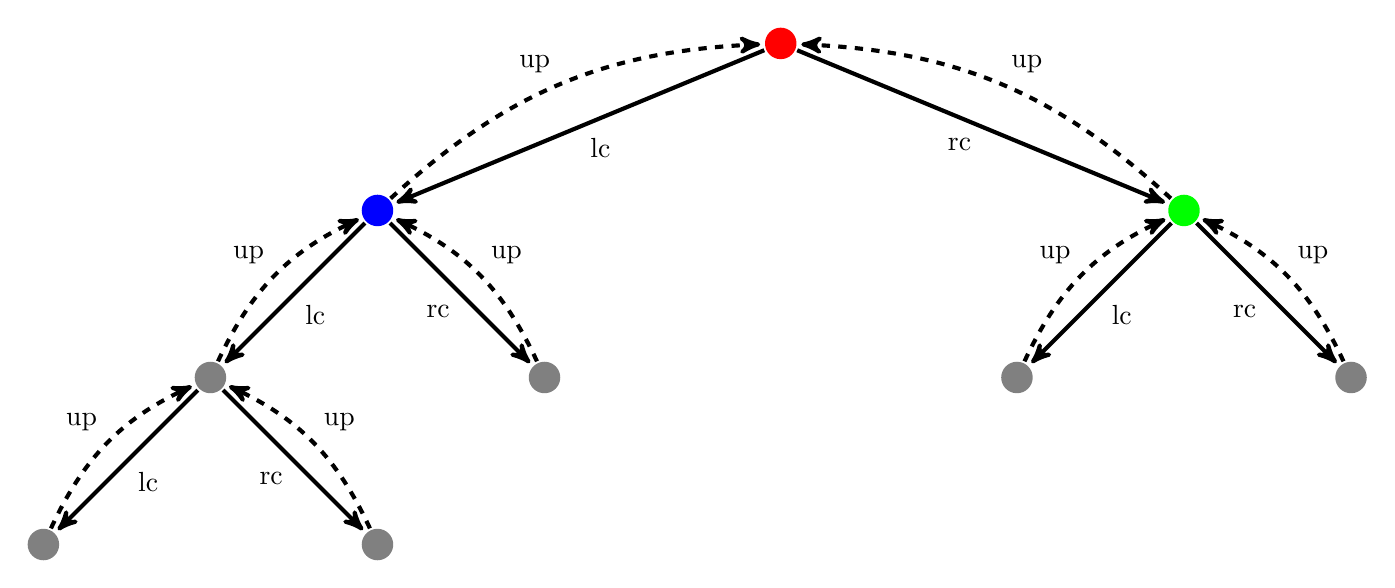
\begin{tikzpicture}[->,>=stealth',shorten >=1pt,auto,node distance=3cm,
                    thick, bend angle = 20,line width = 1.5pt]
  \tikzstyle{every state}=[fill=gray,draw=none,text=white,inner sep=0pt, minimum size=0.4cm]

\tikzstyle{r}=[fill=red]
\tikzstyle{b}=[fill=blue]
\tikzstyle{g}=[fill=green]
  
  {\node[state,r] (r)    {};}
  
   {\node (x) [below left of = r] {};}
   {\node (y) [below right of = r] {};}
   
  {\node[state,b]         (0) [ left of=x] {};}
  
  {\node[state,g]         (1) [ right of=y] {};}
  
  {\node[state]         (00) [below left of=0] {};}
  
  {\node[state]         (01) [below right of=0] {};}

  {\node[state]         (10) [below left of=1] {};}
  
  {\node[state]         (11) [below right of=1] {};}
  
  {\node[state]         (000) [below left of=00] {};}
  
  {\node[state]         (001) [below right of=00] {};}
  
  
  
  \path (r) 
  		edge node {lc} (0)
            	edge [swap]   node {rc} (1)
	(0) 
		edge node {lc} (00)
		edge [swap] node {rc} (01)
		edge [dashed,bend left] node {up} (r)
	(1)
		edge [dashed,bend right, swap] node {up} (r)	
		edge node {lc} (10)
		edge [swap] node {rc} (11)
	(11)
		edge [dashed, bend right,swap] node {up} (1)
		
	(10)  
			edge [dashed,bend left] node {up} (1)
	
	(00) 
		edge node {lc} (000)
		edge [swap] node {rc} (001)
		edge [dashed,bend left] node {up} (0)

	(01) edge [dashed,bend right,swap] node {up} (0)
	
	(000)
		edge [dashed,bend left] node {up} (00)

	(001)
		edge [dashed,bend right,swap] node {up} (00);
		
\end{tikzpicture}


%
%\caption{asdfadfs}


}}
\caption{Reconfiguration problem. Three agents (red, green, blue) find themselves on the internal leaves of some binary tree. Each has the same task: to reach a leaf, different from all the others, in a collision free way. An agent has only a bounded amount of memory, can sense if it is at a leaf, can sense if its left (or right) child is occupied, and can move in three directions, i.e., to the left child, to the right child, or to the parent (dotted arrow). In this example, agents move asynchronously.}
\end{figure}

The aim of this work it to provide a formal framework in which one can reason both mathematically and computationally about multiple mobile-agents moving in partially known environments. In particular, we will define an abstract mathematical model of mobile agents operating in graph-environments, and study the verification problem, i.e., do given agents correctly perform their tasks. 
Our agents are essentially finite-state automata that walk on finite graphs using guarded-commands such as ``if I am north of agent $2$ then step east''. 
We introduce a logic based on linear-temporal logic \LTL for defining agent tasks. This logic is powerful enough to specify standard tasks such as gathering, reconfiguration, and exploration.

We do not model partially-known environments using partial-observability, as is common~\cite{RuNo-AI}. Instead, we
treat the graph-environment as a parameter, e.g., in the reconfiguration example the given agents should achieve their task on {\em all} binary trees, not just the given binary tree. In more detail, fix a class $\gclass$ of environments (e.g., $\gclass$ is the set of all trees, or all grids, or all rings).  The {\em parameterised verification problem (PVP)} states: Given agents $\tup{R}$ and tasks (one for each agent), decide if the agents achieve their tasks on \emph{all} graphs $G \in \gclass$. Since our agents have limited memory, and since there may be infinitely many graphs in $\gclass$, the agents necessarily may only learn a bounded amount of information about the particular graph in which they are deployed, i.e., they have partial information about the graph.  

In contrast, the classic non-parameterised verification problem states: given agents $\tup{R}$ and a graph $G \in \gclass$, decide if agents $\tup{R}$ solve their tasks on $G$. In this setting, the agents can be designed to exploit the exact structure (size, etc.) of the graph, and store all of it in their memory.
% Requiring the agents to solve their tasks on all graphs from a class $\gclass$ is how we model that the agents operate in partially-known environments --- the agents know they are in a graph from $\gclass$, but they do not know which one.
This non-parameterised verification problem is often handled using model-checking~\cite{CGP1999}.  That is, one builds a (potentially very large) finite labeled-transition system representing the global state of the system (i.e., the position and local state of every agent in the given graph $G$), one represents the tasks in a formula of a suitable logic (such as linear-temporal logic \LTL), and then one checks whether the transition system satisfies the formula. Since all objects are finite, this problem is typically decidable, although its complexity depends on the size of the transition system and the formula, and the complexity class varies depending on the logic.

On the other hand, the parameterised verification problem (PVP) corresponds to a family of model-checking problems (one for each $G \in \gclass$). This family is typically infinite, and thus the PVP can be seen as model-checking an infinite-state model (consisting of the disjoint union of the infinitely many finite-state systems). A variety of techniques have been applied to verify certain infinite-state systems, and we discuss these in Section~\ref{sec:related} (Related Work). However, before this work, none seem suited to the problem in which the environment is parameterised.

%Our objective is to formalise and study the parameterised verification problem where it is the environment/graph that is parameterised.

%\begin{example}
% Suppose $k$ many agents have to collaboratively explore an unknown graph. Each agent can  move based on its current local state and the direction in which it entered the current vertex. This problem is known as exploration on anonymous networks \cite{}.
%\end{example}


%A consequence of our main decidability result (Theorem~\ref{thm:PVPdec}) is that, for a fixed task such as reconfiguration or exploration, and a fixed bound $b \in \nat$, one can verify if $k$ given agents can achieve their task (on certain classes of graphs, including lines, trees, rings, and series parallel-graphs, but not grids) with each agent taking at most $b$ turns. A consequence of our undecidability result (Theorem~\ref{thm:PVPundec}) is that this problem is undecidable on lines in the case that there is no assumed bound $b$, and even if one only allows ``local'' testing, i.e., actually we only need to allow a agent to learn which other agents share its current position.



%A agent moves autonomously from vertex to vertex of a finite graph by following a protocol: it consults its  memory, i.e., its internal state, as well as local information about its current position (e.g., a fixed labeling of the current vertex, the degree of the vertex it is currently at, some information about the location of the other agents); based on this information it moves in some direction  (e.g., left, right, up, down), and changes its internal state. The more general \emph{whiteboard model} allows a agent visiting a vertex to read and write from a variable stored at that vertex.
%A weak version of a whiteboard is a {\em pebble} which a agent may drop or retrieve from vertices of the graph.
%We consider the case of identical agents.





% Our work can be seen as a chapter about graph-walking automata. The main novelty in the respect is that our automata are not meant to be graph-acceptors, as is traditional, but rather are meant to do something on the graph. Thus, it is the {\em behaviour/runs} of these automata that this paper analyses.

%Since agents move without central control, the area RAG is part of the field of distributed computing.
%For instance, positive results are of the form ``There is a agent with $f(\Delta)$ states that solves a certain task on all graphs of max degree $\Delta$" and impossibility (and negative) results of the form ``There is no agent (with $f(\Delta)$ states) that solves a certain task on all graphs of max degree $\Delta$".\sr{keep last sentence? or does it set up too high expectations?}
% {follow in the tradition of rigorous systems engineering and}

%However, until recently~\cite{KoLo13AAMAS,ABCTU13,MPST14,KoLo15} there has been little emphasis on formal analysis of correctness of agents in a parameterised setting. In this paper we apply formal methods to the parameterised verification problem in which it is the {\em environment that is parameterised}. This is how we model that agents operate in unknown environments. Formally, we address the following decision problem.
%
%{\bf Parameterised Verification Problem}: Given agents $\tup{R}$, decide if they solve the task $\T$ on all graphs $G \in \gclass$.

%Note that requiring that the agents solve the task $\T$ on all graphs from a class $\gclass$ is how we model that the agents operate in unknown environments.



%In both these problems we have fixed a set of agent protocols $\rclass$, a set of graphs $\gclass$, and a task $\T$. For instance, $\rclass$ may be all finite-state agent protocols (or all pairs of such agents), $\gclass$ may consist of all graphs of a given degree, and $\T$ may be a task of the form ``some agent infinitely often visits a given subset of the vertices''.

%\sr{perpet explor. may mean visit each vertex infinitely often}
%or additionally halting once every vertex has been visited (exploration with stop), additionally halting at the vertex it started on (exploration with return),
%Exploration is often a basic subtask that is useful for more complex tasks \cite{Das13}.


%Typical theorems in RAG are positive results of the form ``There is a agent with $f(\Delta)$ states that solves a certain task on all graphs of max degree $\Delta$", and negative results of the form ``Every agent that solves a certain task on all graphs of max degree $\Delta$ has at least $f(\Delta)$ states", or impossibility results of the form ``There is no agent with finitely many states that solves a certain task on all graphs of max degree $\Delta$". Graph-parameters besides max degree $\Delta$ may also used, e.g., the size $n$ of the graph, the diameter $D$ of the graph. See for instance \cite{KKR06, GR08, Diks200438, Das13,Cohen05graphexploration}. The agent is required to succeed on {\em all graphs} from the (typically infinite) class of graphs.



%The non-parameterised verification problem is often handled using model-checking~\cite{CGP1999}.  The parameterised verification problem corresponds to a family of model-checking problems (one for each $G \in \gclass$), or equivalently, a single infinite-state model-checking problem. A variety of techniques have been applied to such systems, fully discussed in Section~\ref{sec:related} (Related Work),
%however none seem suited to the problem in which the environment is parameterised.
%Fortunately, the theory of automata and logic has produced a rich understanding of the expressive power of certain logics, e.g., monadic second-order logic $\msol$, over certain classes of graphs, e.g., context-free sets of graphs \cite{Thomas90, Thomas96, ALG01, CE12}. Our framework reduces the parameterised verification problem to classic questions in automata theory and $\msol$, i.e., universality and validity problems. The key observations are that: i) agents are graph-walking automata, and can be defined in $\msol$, and ii) agent tasks correspond to properties of runs of automata which are often definable in $\msol$.

%\paragraph{Modeling Choices} \label{modeling}There are a number of different modeling choices for mobile agents \cite{Pelc11}. We list them, and emphasise (using underlining) the choices made in this paper: (i) is the environment continuous (e.g., the plane) or \underline{discrete} (e.g. a finite graph whose edges are labeled by directions or port numbers)? (ii) do agents act \underline{synchronously} or asynchronously? (iii) are agents probabilistic or \underline{non-deterministic}? (iv) is there \underline{one} agent or are there \underline{multiple} agents, and are the number of agents \underline{known} or unknown? (v) is the environment \underline{static}, or can agents affect their environment (e.g., by marking the nodes of a graph)? Moreover, (vi) how much information about the environment is known, a priori, to the agents?  We assume agents \underline{do not have global knowledge} of the environment, and in particular the size is not known and nodes in the environment do not have unique identifiers. And finally, (vii) how do agents communicate and sense their environment? We assume agents can {\em sense their positions in the graph} as well as those of the other agents (in the case of multiple agents), i.e., agents acquire information about the current state of the environment solely by vision (we use logical formulas, which we call tests, to define these sensing abilities).

%\sr{for different modeling choices, does the reduction fail? or just decidability?}

% \sr{what about open systems? in which agents are given new tasks as time goes on} We discuss other modeling choices in Section~\ref{sec:discussion!!}.
% \paragraph{Non-Static Environments}
%Allowing the agents to read and write $b \in \nat$ bits at each vertex (the $b$-bit \emph{whiteboard} model) results in undecidable PVP even for $b=1$, lines, and reachability tasks, cf. \cite{Suzuki}.




%
%Here is the suggested methodology for solving the parameterised verification problem for finite-state agents in the basic model (no whiteboards). First we establish that validity of a certain logic $\L$ over a certain class of graphs $\gclass$ is decidable. \sr{give exs}. Second, we find a (computable) translation of a agent protocol $R$ and task $T$ into a logical formula $\varphi_{R,T}$ such that for every graph $G$, protocol $R$ solves the task $T$ on graph $G$ if and only if $G$ satisfies $\varphi_{R,T}$. Thus, $R$ solves the task $T$ on all graphs from $\gclass$ if and only if every graph in $\gclass$ satisfies $\varphi$.  In other words, solving questions of the form ``Does this agent solve this task on all graphs from class $\gclass$?" is reduced to a problem of the form ``Is a certain formula (that depends on the agent and the task) true on every graph from class $\gclass$?". Thus we might call this the {\bf agent\&task-as-formula} paradigm.

\

\head{Contributions.}
We provide a formal framework for reasoning about multiple mobile-agents on partially-known environments. 
We make the following modeling choices:
\begin{itemize}
 \item environments are finite and discrete (rather than continuous),
 \item agents have finite memory (rather than being Turing powerful),
 \item each agent has its own task to complete (rather than having just a single co-operative task),\footnote{Note, however, that many cooperative tasks can be naturally expressed by specifying the induced individual goals.}
 \item agents are deterministic or nondeterministic (rather than probabilistic),
 \item the number of agents is fixed and arbitrary (rather than unknown),
 \item agents have unique identifiers that may be used (rather than required to be anonymous),
 \item although environments are partially-known agents can test their own positions in the graph using a quite powerful logic, and they have powerful communication abilities: they can choose to publish their states and current/visited positions to a ``bulletin-board'' that can be read by all agents; this allows agents to communicate without being in the same node, i.e., ``remote tests'',
 \item agent communication and testing is completely reliable (rather than being error prone),
 \item environments are static, i.e., agents cannot leave information at visited positions,
 \item agents move asynchronously rather than synchronously (this it motivated by the fact that distributed systems need not have a common notion of time~\cite{Lynch96}).
%  \item \sr{how to describe and motivate the fact that any number of agents can move at a time?} \sout{agents move asynchronously, rather than synchronously.}
%  \footnote{The assumption that agents move asynchronously is motivated as follows: processes in distributed systems have no common notion of time since they may be running with different internal clocks, and thus a standard abstraction is to assume that processes' actions are interleaved \cite{Lynch96}. There are two main ways to interleave the agents: an adversary tries to make sure that the agents do not succeed \cite{FPSW99}, and a co-operator tries to help the agents succeed (reminiscent of schedulers in strategic reasoning \cite{CLMM14}).}
\end{itemize}


This framework allows us to model systems of multiple mobile agents, as well as reason about the border between decidable and undecidable verification problems. There are three main dimensions of an agent system that one can vary to try get decidability: a) the sets of graph-environments, b) the testing abilities of the agents, c) the communication abilities of the agents.\footnote{Actually, one may also restrict the movement abilities of agents as is done in~\cite{AAMAS16Grids}.}

% This is the approach taken in \cite{??}.} Our framework allows arbitrary sets of graphs, very powerful testing abilities (i.e., agents can test their own positions in graphs using a powerful logic, i.e., \msol), c) agents can publish their current position, state, and positions visited so far, and other agents can read and act on this data.

\emph{Undecidability Results.}
Parameterised verification is undecidable already for very simple systems. For a single agent, we get undecidability on grids, even if the agent has very limited testing abilities (i.e., border-detection). For multiple agents, parameterised verification is undecidable already on lines, even if agents have the same limited border-detection testing abilities, and their communication is very limited (i.e., they ``communicate'' by collision-detection). We prove these results by showing how to simulate two-counter machines, a Turing-complete model of computation.

\emph{Decidability Results.}
In order to regain decidability we make the following two restrictions: a) we consider graph-environments that are definable in monadic second-order logic and are of bounded clique-width. We call these \emph{\courcellian} classes of graphs after Courcelle's Theorem (see Theorem~\ref{thm:courcelle}). These are classes of graphs that are in analogy to the context-free languages. They exclude the set of grids, but include, e.g., the set of lines, the set of trees, and the set of cliques; and b) we require that each agent 
may publish its current state and position (which other agents can test) at most a bounded number of times. 

This decidability result is very robust: (i) removing either of the two restrictions, a) or b), results in undecidable parameterised verification; (ii) the decidability result also holds with very powerful agent abilities called {\em position-tests} which allow each agent to {remotely} test the positions of all the agents using formulas which include, e.g., the ability to test connectivity, as well as {\em state-tests} that allow each agent to {remotely} test the internal state of the other agents. Moreover, the decidability result holds for tasks that are expressible using a new logic \RLTL\ (Robot \LTL), which can express many natural tasks, e.g., reconfiguration, gathering, and ``safe'' variations (i.e., complete the task without entering dangerous areas of the graph).%; and also there is no restriction on the agents, i.e., they can be arbitrary finite-state machines.

The main novelty of our approach to decidability is to leverage the theory of automata. This theory allows us to reduce our problems to the satisfiability problem of monadic second-order logic $\msol$ over certain classes of graphs, i.e., \courcellian sets of graphs \cite{Thomas90,Thomas96,ALG01,CE12}. The key observations are that: i) agents are graph-walking automata, and can be defined in $\msol$, and consequently we can permit agents to test the current state of the system (i.e., the graph and the positions of all the agents) using tests expressible in $\msol$, and ii) agent tasks correspond to properties of runs of automata which are often definable in $\msol$.

\section{Related Work.} \label{sec:related}

\todo{I suggest to refocus the related work to papers in AI}




We begin by describing the connection between this paper and two conference papers it is based on.

\paragraph{Conference versions of this paper}
This paper combines and enhances the full versions of two conference papers, \cite{Rubin15AAMAS} and \cite{RZMA15}. The first paper initiated the idea of using automata 
theory and logic to reason about parameterised verification where the environment is the parameter. Its decidability result (and the corresponding logic for expressing tasks) is for single agent systems, and its undecidability result is for two agents that move  synchronously and use remote tests. The second paper extends the first: the decidability result is for multiple asynchronous agents with very powerful remote testing abilities and a necessary restriction on the asynchronous scheduling of the agents, and its undecidability result is for agents that only need local testing abilities, i.e., the ability to detect which other agents they collide with. 

In this full version we supply a cleaner formalism, including a user-friendly logic for expressing agent tasks; we generalise the decidability result from bounded-switching to bounded-publishing, and from asynchronous scheduling to both synchronous and asynchronous scheduling (and anything in between), and to allow agents to test the set of positions that others have accumulated during the run; 
and we correct some minor mistakes.

\iffalse
Systems are considered distributed if they do not have a central control. In light of this, we describe the relationship of our work to formal verification of distributed systems, as well as to work on verification of agent protocols in particular. 

\paragraph{Formal verification of distributed systems}

Typical parameters that arise in the study of distributed systems are the number of agents, the number of assumed faulty agents, etc. Since parameterised problems of distributed systems are, in general, undecidable~\cite{AK86,Suzuki}, the formal methods community developed sound but incomplete methods that require human intervention, e.g., counter- and predicate-abstractions, inductive invariants, regular model checking and acceleration techniques. See for instance~\cite[references on pages 2-3]{PXZ02}.

On the other hand, by simplifying the systems  (e.g., restricting the mode of communication, the abilities of the processes, the specification languages, etc.) one can get decidable PVP. These use techniques from games, automata theory and logic, notably finite-model properties/cutoffs, reduction to Petri nets, and the theory of well-structured transition systems~\cite{GS92,EN95,EsparzaFM99,EmersonK03LICS,CTTV04,KoLo13AAMAS,Delz14,AJKR14,DBLP:conf/icalp/AminofRZS15,AKRSV17}.


The formal-verification community has placed emphasis on distributed models in which processes are stationary and interact by sending messages (e.g., in a broadcast or rendezvous manner) or by using guarded commands. Having said that, token-passing systems (i.e., the models in \cite{EN95,CTTV04,AJKR14,AKRSV17}) are the closest to agents --- both tokens and agents move along the vertices of graphs. However, we now argue that the model in these cited papers is incomparable with our model. First, the translation of their token-passing systems into agent systems would require that agents can read and write to variables at the vertices (this is to model the fact that processes have states). However, we assumed environments are static (because otherwise the PVP is quickly undecidable). Conversely, translating agent-systems into the cited token-passing systems requires that the agent-systems satisfy the following unrealistic assumptions (that are used in their decidability proofs): when an agent decides to move, an adversary decides which edge it takes, as well as to which of its internal states to transition (i.e., even the agent's memory may be scrambled). Not even the simplest robots from the distributed computing literature 
(e.g., the robots from section~\ref{sec:illustration})  satisfy this double restriction.

\fi

\todo{remove next par?}
\paragraph{Mobile agents in the distributed-computing literature.}
The distributed-computing community has proposed and studied a number of models of mobile agents systems, which they call \emph{robots}, e.g., recently
\cite{Bender20021,KKR06,GR08,Das13,Diks200438,Cohen05graphexploration,FIPPP04}. This literature is mostly mathematical, and {\em theorems from this literature are parameterised}, i.e., they may involve {graph-parameters} (e.g., the maximum degree, the number of vertices, the diameter), {memory parameters} (e.g., the number of internal states of the robot protocol), and the {number of robots} may be a parameter.
Only recently has there been emphasis on formal analysis of correctness of robots in a parameterised
setting. In these formal analyses, typically it is the {\em number of agents} that is treated as the parameter \cite{KoLo13AAMAS,KoLo13IJCAI,ABCTU13,MPST14,KoLo15,DBLP:journals/ai/KouvarosL16}. In contrast, we apply formal methods to the parameterised verification problem in which it is the {\em environment that is parameterised}.


\paragraph{Formal verification of mobile-agent systems}

% \sr{check for new papers since 2015, e.g., widder et al, FRIDA, waluciewicz}
% Devi11

The formal methods community has begun explicitly verifying and synthesising robot protocols (rather than distributed systems in general)~\cite{HMM11,Bonnet12,Berard13,ABCTU13,DBLP:journals/ipl/CourtieuRTU15,DBLP:conf/wdag/CourtieuRTU16,MPST14,KoLo15}.


Some of these works only treat concrete values of the parameters~\cite{HMM11,Bonnet12,Berard13}. 
% For instance, one such paper concludes
% \cite[page 11]{Berard13}:
% 
% \begin{verbatim}
% While our method is parameterised by both k [the number of robots]
% and n [the size of the graph], it does not permit to verify whether a
% [robot] protocol is valid for every k and n satisfying a particular
% predicate.
% \end{verbatim}
%
The papers that do treat arbitrary values of the parameters do not give sound and complete decision procedures for their systems, as we do. Indeed, \cite{ABCTU13,DBLP:journals/ipl/CourtieuRTU15,DBLP:conf/wdag/CourtieuRTU16} use a proof assistant to provide certificates (formal proofs) of impossibility results about robot networks and swarms; \cite{MPST14} uses the theory of games on graphs to synthesise a robot protocol for gathering $k$ robots on a ring of size $n$ (for small values of $k,n$), and relies on a hand-proven induction to prove that the synthesised robot protocol works for all values of the parameters $k,n$; and \cite{KoLo15} presents a sound technique that may identify cutoffs using a counter-abstraction in order to draw conclusions about certain swarm algorithms, independently of the number of swarming agents.
%\sr{mention Allessio's work? they DO PV, but is it robots really?}

% The quotation above continues:
% \begin{verbatim}
% Adapting recent advances in parameterised model checking
% [citation elided] would be a nice way to obtain such results.
% \end{verbatim}

In contrast, our methodology, i.e., reducing parameterised verification of robot systems to satisfiability problems in logic, allows us to establish decidability, i.e., sound and complete algorithms for solving the parameterised verification problem for certain classes of robots and environments.
% and have succeeded where other methods and ``recent advances'' (discussed in the previous subsection) have not.




\paragraph{Automata on words, trees, and graphs}
Our model of a single agent protocol is similar to graph-walking automata with $\msol$-tests~\cite{BlEn97}. The proof idea of Lemma~\ref{lem:zeta} (which compiles agents into formulas over graphs) is inspired by \cite{BlEn97,EnHo06}. Other classical notions of automata on graphs (e.g., \cite{BlHe67}) are often too expressive and lead to undecidable parameterised verification problems (see the proof of Theorem~\ref{thm:undec-1robotgrid}). Distributed graph automata~\cite{DBLP:conf/lics/Reiter15} are a model of computation that mimic synchronous distributed algorithms and are used as graph acceptors, and are equivalent to \msol on finite graphs.

% On the other hand, when restricted to words and trees, there are classical and robust notions of automata, i.e., word- and tree-automata \cite{comon2007tree}. A single robot protocol operating on a word (or tree) can be thought of as a two-way automaton (tree-walking automaton). Two way-automata are classical objects that only define the regular languages but are exponentially more succinct \cite{HMU03}. \sr{where is succinctness proven} Tree-walking automata, and their corresponding regular expressions, have been studied for their own sake \cite{Boja08}, in formal verification, e.g., \cite{Vardi98,BLMV08,Obdr13}, and as tree pattern-matching tools \cite{BrWo00,Schw12}. We use them in Theorem~\ref{thm:exptime} to reason about a single robot on an unknown tree.

% \sout{The walking-automata just discussed have a single moving head. Similarly then, multiple (finite-state) robots operating on words resemble multi-head automata, i.e., read-only Turing machines with multiple heads and a single tape. Indeed, it is not hard to see that the universality problem for such automata (i.e., decide whether a given multi-head automaton accepts all words) is equivalent to the parameterised verification problem for multiple robots operating synchronously on line-environments with the ability to communicate their local states to each other, and with reachability tasks (cf. the proof of Theorem~\ref{}). On the other hand, the restrictions we provide on robot systems that ensure decidability of PV thus yield a class of multi-head automata with decidable universality.\sr{CHECK}
% Logical aspects of multi-head automata have been studied in \cite{}.}




% \paragraph{Synthesis}
% Synthesis, the ``big-brother'' of verification, is the problem of automatically producing systems (in our case, robots) that correctly perform the required tasks. There is a smattering of work on parameterised {\em synthesis} of distributed systems (not neccessarily robot systems). In the AI literature this is called {\em generalised planning}:
% \cite{GFPS10,HuG11,GMRS16IJCAI}. These papers deal with one agent in a parameterised environment. In the verification literature \cite{KJB13CAV,KJB13VMCAI} show \todo{???}
% 
% \todo{discuss \cite{MPST14} and \cite{KoLo15}.}

%\item Regular expressions for two way automata \cite{BrWo00}
%\item Tree walking automata, graph-walking automata, and multi-head TWA/GWA \cite{Boja08,Vardi98}
%\item graph walking automata \cite{BlHe67}
%\item reversal bounded multi-counter machines \cite{Ibarra78JACM}
%\sr{should we mention bounded context-switching multi stack machines \cite{QaRe05}?}
%\item stack ordered machines \cite{}
%\item timed automata with stopwatches \cite{}
%\item {In some work, this setting is described as being {\em online}, in the sense that the robots have to react to the environment as they discover it, rather than {\em offline} in which they can plan to achieve their task on a fixed environment \cite{}.}

%For a detailed discussion relating these models (especially the token-passing systems) to multi-robot systems, see the Related Work in \cite{Rubin15AAMAS}.






%
%\begin{itemize}
%\item Undecidable cases:
%\begin{enumerate}
%\item 2 robots on a line, synchronous time, each robot can test itself or the other robot for being at the left and right end of the line, reachability objective, (2CM).
%\item 2 robots on a tree, synchronous time, each robot can test the position of any other robot (is it at the root? is it at a leaf? is it at the $i$th child of its parent?), reachability objective (2CM).
%\item 3 robots on a tree, synchronous time, robots can only move down tree, robots have collision detection, robots ca test positions (ie., each robot can detect whether a given robot is in the left-child, the right-child, the root, or a leaf),
%reachability objective (PCP problem).
%\item 10 robots on a line, asynchronous time, collision detection, left/right position test, reachability objective (simulate synchrony).
%\end{enumerate}
%
%\item Decidable cases:
%
%\begin{enumerate}
%\item multiple robots on tree-like structures, asychronous time, bounded context-switching, MSO-tests, MSO-objectives (generalises AAMAS paper). \sr{A slight generalisation is this is also decidable: only runs that are considered are those that can be split into $N$ phases (for some fixed $N$), and at each phase there is some subset of robots $F$ that are frozen (i.e., they do not act) and every robot not in $F$ can move as it likes, but can only test the position of itself and the position of robots in $F$ (i.e., robots not in $F$ can not test the positions of other robots not in $F$).}
%\item multiple robots on a line or a grid, synchronous time, reversal bounded movement, collision detection.
%\item multiple robots on a tree, synchronous time, only the largest numbered robot not at the root can move towards the root, robots can test positions (adding collision detection results in undecidability, see above).
%\item one robot on a tree, with MSO tests, and a finite set of nested pebbles that it may drop and pickup.
%\end{enumerate}
%
%\item Unclear cases:
%\begin{enumerate}
%\item nested automata
%\end{enumerate}
%\end{itemize}



\section{Background}  \label{sec:prelim}
We will use basic notions from mathematical logic including monadic second-order logic~\cite{EbFl95}, automata theory~\cite{HMU03}, 
and linear-temporal logic~\cite{CGP1999}. We will introduce them below, as needed.
%, and the theorem of McNaughton and Papert connecting star-free languages and first-order logic, see~\cite{Thomas96})
%
Write $B^\omega$ for the set of infinite sequences over alphabet $B$, and write $B^*$ for the set of finite sequences. The empty sequence is denoted $\epsilon$.
Sequences are indexed starting at $0$, thus we write $\alpha = \alpha_0 \alpha_1  \cdots$. 
Write $[n]$ for the set $\{1,2,\cdots,n\}$.

\todo{In the rest of this paper we use the term ``robot'' instead of ``mobile agent''.}

% The reader may refer to this section as needed.
\subsection{Graphs, \LTL and \msol} \label{subsec:graphs-MSOL}

\head{Graphs.} Graphs will serve as the environment in which robots move.
Let $\Sigma$ be a finite set of {\em edge labels}.
A {\em $\Sigma$-graph}, or {\em graph}, $G$, is a tuple $(V,\lambda)$ where $V$ is a finite set of {\em vertices} and $\lambda:V^2 \to \Sigma$ is a partial function called the {\em edge labeling function}. The domain of $\lambda$ is denoted $E \subseteq V \times V$, and is called the
{\em edge relation}. We write $\trans{v}{w}{\sigma}$ to mean $\lambda(v,w) = \sigma$.
A graph is \emph{deterministic} if for every $v \in V, \sigma \in \Sigma$ there exists at most one $v'$ such that $\lambda(v,v') = \sigma$. Here are some examples of classes of deterministic graphs.

% \sr{Q: do we want to consider nondeterministic graphs? what about vertices from which there may not be an edge labeled $\sigma$?}

%The {\em out-degree} of a vertex $v$, written $\deg(v)$, is the cardinality of the set $\{(v,w) \in E : w \in V\}$ of {\em outgoing edges} of $v$.
%
%Sometimes the edge labels give a sense of direction:
%
%\begin{example} An {\em $L$-labeled grid} is a graph with $V = [n] \times [m]$, $\Sigma =  L \times \{N,S,E,W\}$, and labels $\lambda((x,y),(x+1,y)) \in L \times \{E\}$, etc., where $L$ is a finite set and $n,m \in \nat$. An {\em $L$-labeled line} is an $L$-labeled grid with $V = [n] \times [1]$. If $|L| = 1$ then we call the grid (or line) {\em unlabeled}.
%\end{example}
%


% \label{ex:tree}
\head{Trees.} A {\em $\Delta$-ary tree} (for $\Delta \in \nat$) is a $\Sigma$-graph $(V,\lambda)$ where $(V,E)$ is a tree, $\Sigma = [\Delta] \cup \{up\}$, and $\lambda$ labels the edge leading to the node in direction $i$ (if it exists) by $i$, and the edge leading to the parent of a node (other than the root) is labelled by $up$. We may rename the labels for convenience, e.g., for binary trees ($\Delta = 2$) we let $\Sigma = \{lc,rc,up\}$ where $lc$ replaces $1$ and $rc$ replaces $2$. For instance, see Figure~\ref{fig:tree}.

\head{Lines.} The \emph{$n$th line} is the $\Sigma$-graph $L_n = (V_n,\lambda_n)$, where $\Sigma = \{l,r\}$, $V_n = [n]$, and $\lambda_n(i,i+1) = r$ and $\lambda_n(i+1,i) = l$. Thus, the domain of $\lambda_n$ is  $E_n = \cup_{i,j \in [n]} \{(i,j) : |i-j| = 1\}$. \label{def:line}

\head{Grids.} The \emph{$n$th grid} is the $\Sigma$-graph $G_n = (V_n,\lambda_n)$, where $\Sigma = \{u,d,l,r\}$, $V_n = [n] \times [n]$,  and the labels are as expected with $u$ standing for ``up'', $d$ for ``down'', $l$ for ``left'' and $r$ for ``right''. E.g., $\trans{(i,j)}{(i+1,j)}{r}$ and $\trans{(i,j)}{(i,j+1)}{u}$.
% Thus the edge relation $E_n$ consists of all pairs $((i,j),(i',j'))$ such that $|i-i'| = 1$ xor $|j = j'| = 1$.

%A $\Delta$-ary tree with $\Delta = 1$ is called a {\em line}. A $\Delta$-ary tree in which every vertex has degree at most $2$ is called a {\em labelled line}.


% The degree of a graph $G$ is the maximum degree of all its vertices.


% To simplify the presentation we do not distinguish between the syntactic symbols used in formulas (such as the binary relation symbol $E$) and the semantic symbols used in structures; thus, e.g., we write the formula $E(x,y)$ where $E$ is a binary relation symbol, as well as the expression $(u,v) \in E$ where $E$ is the edge relation of a graph.


\head{Linear Temporal Logic.} \label{dfn:LTL}
This is a canonical modal logic for the specification of reactive systems. Here we will use it as a foundation for specifying robot tasks.

For a set of \emph{atoms} $\AP$, write $\LTL(\AP)$ (or simply \LTL) for the logic with the following syntax and semantics:
$\varphi ::= p \mid \varphi \wedge \varphi \mid \neg \varphi \mid \nextX \varphi \mid \varphi \until \varphi$, where $p$ varies over $\AP$.
We use standard abbreviations, e.g., $\false := p \wedge \neg p, \true := \neg \false, \eventually \varphi := \true \until \varphi$,
	$\always \varphi := \neg \eventually \neg \varphi$, etc.
% 	 $\varphi \weakuntil \varphi' := (\varphi \until \varphi') \vee \always \varphi$,
	The \emph{safety} formulas are those of the form $\always b$ where $b$ is a Boolean combination of atoms.
	
	
	Formulas are interpreted over infinite strings $\alpha = \alpha_0 \alpha_1 \alpha_2 \cdots \in (2^\AP)^\omega$. Define the satisfaction relation
	$\models_\LTL$ as follows:
	\it
	\- $(\alpha,n) \models_\LTL p$ iff $p \in \alpha_n$;
	\- $(\alpha,n) \models_\LTL \varphi_1 \wedge \varphi_2$ iff $(\alpha,n) \models_\LTL \varphi_i$ for $i = 1,2$;
	\-	$(\alpha,n) \models_\LTL \neg \varphi$ iff it is not the case that $(\alpha,n) \models_\LTL \varphi$;
	\-  $(\alpha,n) \models_\LTL \nextX \varphi$ iff $(\alpha,n+1) \models_\LTL \varphi$;
	\- $(\alpha,n) \models_\LTL \varphi_1 \until \varphi_2$ iff there exists $i \geq n$ such that $(\alpha,i) \models_\LTL \varphi_2$ and for all $i \leq j < n$, $(\alpha,j) \models_\LTL \varphi_1$.
	\ti
	Write $\alpha \models_\LTL \varphi$ if $(\alpha,0) \models_\LTL \varphi$ and say that $\alpha$ \emph{satisfies} $\varphi$.



  \head{Monadic Second-order Logic.} \label{dfn:msol} This is an extension of first-order logic by set variables. It will be used to define powerful testing abilities of robots, as well as a technical tool in the decidability proofs.

Formulas are interpreted in $\Sigma$-graphs $G$. Define the set of monadic second-order formulas $\msol(\Sigma)$ as follows. Formulas of $\msol(\Sigma)$ are built using {\em first-order variables} $x,y,\cdots$ that vary over vertices, and {\em set variables} $X,Y, \cdots$ that vary over sets of vertices. The {\em atomic formulas} (when interpreted over $\Sigma$-graphs) are:
\it
\- $x = y$ (denoting that vertex $x$ is the same as vertex $y$),
\- $x \in X$ (denoting that vertex $x$ is in the set of vertices $X$),
% \- $init(x)$ (denoting that $x$ is the initial vertex $v_0$), and
\- $\lambda(x,y) = \sigma$ (denoting that there is an edge from $x$ to $y$ labeled $\sigma \in \Sigma$).
% \- $\true$ (the formula that is always true).
\ti
The formulas of $\msol(\Sigma)$ are built from the atomic  formulas using the Boolean connectives (i.e., $\neg,\vee, \wedge, \limp$) and variable quantification (i.e., $\forall,\exists$ over both types of variables). The fragment of $\msol(\Sigma)$ which does not mention set variables is called {\em first-order logic}, denoted $\fol(\Sigma)$.
Write $\msol_k(\Sigma)$ for formulas with at most $k$ many free first-order variables and no free set-variables. We abbreviate $z_1, \cdots, z_k$ by $\tup{z}$. We write $\phi(x_1, \cdots, x_k)$ to mean that the free variables from the formula $\phi$ are amongst the set $\{x_1, \cdots, x_k\}$. Note that the formula $\phi(x_1,\cdots,x_k)$ does not need to use all the variables from the set $\{x_1,\cdots,x_k\}$. When $\Sigma$ is clear from the context, it may be dropped.

The semantics of \msol is defined in a similar way as for first-order logic. Instead of giving the formal definitions (see~\cite{EbFl95}) it is enough to introduce some useful notation. Given a graph $G$, a \emph{valuation $\nu$} is a function that maps each first-order variable to a vertex in $G$ and each monadic second-order variable to a set of vertices of $G$. Thus, we write $(G,\nu) \models \phi(x_1,\cdots,x_k,X_1, \cdots, X_l)$ to mean that $\phi$ holds in $G$ with variable $x_i$ (resp. $X_i$) simultaneously substituted by vertex $\nu(x_i)$ (resp. $\nu(X_i)$).
A {\em sentence} is a formula with no free variables. In this case we write $G \models \phi$ to mean that $\phi$ holds in $G$. A sentence $\phi$ is \emph{satisfiable} if there exists a graph $G$ such that $G \models \phi$.



%  A sentence $\phi$ is \emph{valid} if for all graphs
%  $G$, $G \models \phi$.
% \sr{remove dfns of sat and valid if they are not needed}


%\footnote{In the section on \RLTL\ we will introduce the satisfaction relation $\models_{\tup{R},\Omega}$.}

Here are some examples of formulas and their meanings:
\example{\label{ex:formulas}
\begin{itemize}

% \item  We abbreviate $\bigwedge_i x_i = y_i$ by $\tup{x} = \tup{y}$, and $\bigwedge_i x_i \in X_i$ by $\tup{x} \in \tup{X}$.

\item The formula $\forall x (x \in X \limp x \in Y)$ means that $X \subseteq Y$. Similarly, there are formulas for the set operations $\cup, \cap,=$, and relative complement $X \setminus Y$.

 \item The formula $E(x,y) := \bigvee_{\sigma \in \Sigma} \lambda(x,y) = \sigma$ says that there is an edge from $x$ to $y$.

 \item On lines (so $\Sigma = \{l,r\}$) the formula $\neg \exists y. \lambda(x,y) = r$ states that $x$ is on the right end-point of the line.

 \item On binary-trees (so $\Sigma = \{lc,rc,up\}$) the formula $\neg \exists y. \lambda(y,x) = up$ states that $x$ is a leaf, $\neg \exists y. \lambda(x,y) = up$ states that $x$ is the root, and $\exists y. \lambda(y,x) = lc$ states that $x$ is a left-child.

%\item The formula $\exists x \exists y (x\neq y \wedge  edg(z,x) \wedge edg(z,y))$ means that $\deg(z) \geq 2$.
 \item The formula $E^*(x,y) := \forall Z [(closed_{E}(Z) \wedge x \in Z) \limp y \in Z]$ defines the transitive closure of $E$, where $closed_{E}(Z)$ is $\forall a \forall b[(a \in Z \wedge E(a,b)) \limp b \in Z]$.


%  $\phi^*(x,y)$ holds in a graph $G$ if and only if there exists a finite sequence of vertices $v_1 v_2 \cdots v_m \in V^*$  (here $m \geq 1$) such that $x = v_1, y = v_m$ and $\phi(v_i,v_{i+1})$ holds in $G$ for all $i < m$ (for example, if $\phi(x,y) = edg(x,y)$ then $G \models \phi^*(x,y)$  if and only if $G$ has a path from $x$ to $y$). This shows that that if a binary relation is $\msol$-definable, then so is its transitive-closure.
% %%Write $[[\phi]]_G := \{\tup{v} \in V^k : G \models \tup{v}\}$.
%%We say that a graph $G$ {\em satisfies} a sentence $\phi$, and write $G \models \phi$, if $\phi$ is true in the graph $G$.
\end{itemize}
}
% of $\msol$-definable formulas \label{ex:TC} \begin{itemize}
%\item
%
%
%
%%Similarly, $\phi^+(x,y) := \exists z (\phi(x,z) \wedge \phi^{*}(z,y))$ is as before, but replace $m \geq 1$ by $m > 1$.
%\item Similarly, define $\phi^\omega(x,y) := \phi^*(x,y) \wedge \exists z (\phi(y,z) \wedge \phi^{*}(z,y))$. Note $\phi^\omega(x,y)$ holds in a graph $G$ if and only if there is an infinite sequence of vertices $v_1 v_2 \cdots \in V^\omega$ with $x= v_1$, $v_i = y$ for infinitely many $i \in \nat$, and $\phi(v_i,v_{i+1})$ holds in $G$ for all $i \in \nat$. This uses the fact that $V$ is finite.
%
%\item Note that if $\phi(x,y,\tup{z})$ is an $\msol(\Sigma)$ formula we can define an $\msol(\Sigma)$ formula $\phi^*(x,y,\tup{z})$ that expresses  that there exists a finite sequence of vertices $v_1 v_2 \cdots v_m \in V^*$  (here $m \geq 1$) such that $x = v_1, y = v_m$ and $\phi(v_i,v_{i+1},\tup{z})$ holds in $G$ for all $i < m$. In other words, we can treat $\tup{z}$ as parameters. We can similarly add parameters to $\phi^\omega$.
%\end{itemize}

%no space
%\item[MF5.] \label{ex:ktc}


%The set of formulas in $\fotc(\Sigma)$ is defined to be the set of formulas $\fol(\Sigma)$  closed under the transitive-closure operator (for $k=1$). We have seen that every formula in $\fotc(\Sigma)$ is expressible as a formula in $\msol(\Sigma)$, which justifies writing $\fotc(\Sigma) \subset \msol(\Sigma)$, a slight abuse of notation. \sr{is FOTC used?}






%\subsection{Automata and Regular Expressions.}
%\sr{define automata? universality problem?}
%
% Ordinary {\em regular-expressions} over a finite alphabet $B$ are built from the
% sets $\emptyset$, $\{\epsilon\}$, and $\{b\}$ ($b \in B$), and the operations
% union $+$, concatenation $\cdot$, and Kleene-star $\phantom{}^*$.
% Kleene's Theorem states that the languages definable by regular expressions over
% alphabet $B$ are exactly those recognised by finite automata over alphabet $B$.


%
% An {\em $\omega$-regular expression} over alphabet $B$ is inductively defined to
% be of the form: $exp^\omega$, $exp \cdot r$, or $r + r'$, where $exp$ is an
% ordinary regular-expression over $B$, and $r,r'$ are $\omega$-regular
% expressions over $B$. An {$\omega$-regular language} is one defined by an
% $\omega$-regular expression. A variation of Kleene's Theorem says that the
% languages definable by $\omega$-regular expressions over alphabet $B$ are
% exactly the languages recognised by B\"uchi automata over alphabet $B$ (which
% are like finite automata except they take infinite words as input, and a run is successful if
% some accepting state occurs infinitely often).


%A regular language over alphabet $B$ is {\em star-free} if it is the language of a regular-expression over $B$ that does not use the Kleene-star, but may use the complementation operator (written $\neg{r}$).
%A {\em star-free $\omega$-regular language} is the language of an $\omega$-regular expression that may mention the complement operator, but may not mention the $\omega$-power $exp^\omega$ nor the Kleene-star $exp^*$ operators.

\iffalse
We will use the McNaughton-Papert Theorem (and its generalisation to infinite-words) (see \cite{Thomas96,DiGa08}): it states that a regular language of ($\omega$)-words is star-free if and only if it is definable in first-order logic. For instance, the language $0^*1^*$ over alphabet $\{0,1\}$ is definable by the formula $\exists z. \forall x. [x \leq z \limp P_0(x)] \wedge [x \not \leq z \limp P_1(x)]$, and by the star-free regular expression $\neg( \neg{\emptyset} \cdot 1 \cdot 0 \cdot  \neg{\emptyset})$. Formally, a word $w \in B^*$ is coded as a structure with domain $[|w|]$, unary predicates $P_b := \{i \leq |w| : w_i = b\}$ (for $b \in B$), and the usual linear order $\leq$ on $[|w|]$; and thus the first-order definition may make use of these unary predicates and the linear order.
\fi

%\footnote{Although this is the standard encoding, if one prefers uniformity with the earlier definition graph, one may instead code the word $w$ as an edge-labeled graph with $|w|+1$ vertices, and an additional edge label for $\leq$.}

%\sr{use 'FO language' and 'FO models'?}
%Graphs of degree at most $\Delta \in \nat$ will be called $\Delta$-graphs.


\section{The Model of Multi-Robot Systems and Robot Task Logic} \label{sec:model}


In this section we provide a framework for modeling multi-robot systems parameterised by their environment. Here is a brief outline.
%We generalise the definition of robot systems from \cite{Rubin15AAMAS} to allow asynchronous behaviour.
An environment is modeled as a $\Sigma$-graphs $G$, and robots are modeled as finite-state automata over an alphabet of guarded commands.
A guarded command tells the robot to move along an edge with a given label or stay where it is, subject to a test being true.
Robots can test their own current positions, as well as the published positions and local states of other robots. That is, robots can publish their current
position and local state (by entering special `publishing' states) --- this can be thought of as shared memory, or a bulletin-board, where each robot overwrites
its current state and position. Robots move asynchronously, i.e., at least one robot (chosen nondeterministically) moves at a time.
We also provide a definition of a logic, based on Linear Temporal Logic (\LTL), in which one can express various tasks such as gathering, exploring, and reconfiguring.  The logic is called Robot Linear Temporal Logic (\RLTL): it is like \LTL except that its atoms are tests. We assign one \RLTL formula to each robot that specifies its goal, and we require that each of the robots achieve its goal. Thus, co-operative global specifications are given by specifying the individual requirement for each robot.
%e.g., to specify that all robots gather we assign to each robot the individual task of reaching a position containing all the other robots.
% All tests (whether for robots or specfication formula) are based on \msol.
%As discussed in Section~\ref{sec:DC}, our model is general enough to be able to express a popular model of robot systems found in the distributed computing literature~\cite{FIPPP04,Diks200438,Cohen05graphexploration,KKR06,GR08,Das13}.

\subsection{The Model of Multi-Robot Systems}

In the rest of this section, $\Sigma$ denotes a finite set of edge-labels, and $k \in \nat$ denotes the number of robots.

\head{Commands and Tests.}
%
A {\em command} is a symbol from $\upmu(\Sigma) := \{move(\sigma) : \sigma \in \Sigma\} \cup
\{stay\}$.  The command $move(\sigma)$ tells the robot to move
from its current vertex along an edge labeled $\sigma$, and the command
$stay$ tells the robot to stay at its current vertex.

% \sr{should we instead use $pub\_{pos_i}$, $cur\_pos$, $pub\_{st_i}$, $cur\_st$? no.}

% \sr{i changed $cur$ to $pos_{cur}$.}

 A {\em position-test} is a formula $\tau$ from $\msol_{k+1}(\Sigma)$ whose free variables come from the set 
 $\{\VARbcpos_1, \cdots, \VARbcpos_k,\VARpos_{cur}\}$. Informally, a position test
  \[
\tau(\VARbcpos_1,\cdots,\VARbcpos_k,\VARpos_{cur})  
 \]
allows the robot to test that $\tau$ holds in $G$
 where $\VARbcpos_{cur}$ is the current position of the robot doing the testing, and each $\VARbcpos_i$ is the last published position of the $i$th robot.
 Thus, the test $\VARbcpos_i = \VARbcpos_{cur}$ states that the current position (of the robot doing the testing) is equal to the last published position of robot $i$,
 the test $\bigwedge_{i,j} \VARbcpos_i = \VARbcpos_j$ states that the last published positions of all the robots are equal,
 and $E(\VARbcpos_i,\VARbcpos_j) \vee E(\VARbcpos_j,\VARbcpos_i)$ tests if the last published positions of robots $i$ and $j$ are adjacent.

 A {\em state-test} is an expression of the form $st_i = q$, or an expression of the form $st_{cur} = q$, where $i \in [k]$ and $q$ is a symbol representing a state (for concreteness, we may take $q \in \nat$).
 The meaning of $st_i = q$ is that
 the last published state of robot $i$ is $q$, and the meaning of $st_{cur} = q$ is that the current state of the robot doing the testing is $q$.
% For convenience, we assume that all robots have states from $\nat$, i.e., that $q \in \nat$.

% \begin{definition}[Tests]
 The set of \emph{tests for $k$ robots on $\Sigma$-labeled graphs} $\uptau_k(\Sigma)$ is the smallest set containing state-tests, position-tests, and closed under Boolean combinations ($\wedge,\neg$).
% \end{definition}

 For convenience we use the following natural shorthands. If $Q$ is a finite set of states,
 \begin{enumerate}
  \item $\bigvee_{q\in Q} (st_i = q \wedge st_j = q)$ is a test, which is abbreviated $st_i = st_j$. Similarly, we may write $st_{cur} = st_j$.
  \item $\bigvee_{q \in X} st_i = q$ (for $X \subseteq Q$) is abbreviated $st_i \in X$. Similarly, we may write $st_{cur} \in X$.
 \end{enumerate}



 % no space...  Here is a more complex test: is there a path from robot $i$ to
 % robot $j$ that only uses edges labeled $\sigma$? It can be expressed using
 % the transitive closure formula (see Example~MF4 in
 % Section~\ref{sec:prelim}). We emphasise that the test ``$\true$'' is always
 % satisfied.

%
%
% \begin{definition}[Guarded Commands]
The set of {\em guarded commands $\ins$} (which depends on $k,\Sigma$) consists of all expressions of the
form $\gc{\tau}{\kappa}$ where $\tau \in \uptau_k(\Sigma)$ is a test and $\kappa \in \mu(\Sigma)$ is a command.
% \end{definition}

\begin{example}
The guarded command $\gc{(\VARbcpos_1 = \VARbcpos_2 \wedge st_1 = st_2)}{move(u)}$
tells the robot to move in direction $u$ if the last published states and positions of robots $1$ and $2$ coincide.
\end{example}





%For a sequence of instructions $ins \in ((\ins_{\Sigma,k})^k)^*$ define  $[[ins]]_G \subseteq V^{2k}$ such that $(\tup{u},\tup{v}) \in [[ins]]_G$ if and only if, in $G$, one can reach $\tup{v}$ from $\tup{u}$ by successfully executing the instructions in $ins$. To improve readability, the notation $[[\phantom{n}]]_G$ does not mention $k$.
%%
% Formally,\sr{this can be simplified to what is means for one robot to make one move}
%  \begin{enumerate}
%  \item If $ins = \epsilon$, then $(\tup{u},\tup{v}) \in [[ins]]_G$ if and only if $\tup{u} = \tup{v}$;
%  \item If $ins = (d_1,\cdots,d_k) \in (\ins_{\Sigma,k})^k$
%  then $(\tup{u},\tup{v}) \in [[ins]]_G$ if, for each $i \in [k]$, writing $d_i = \tau_i \to \kappa_i$, %\footnote{This is where we introduce the assumption that robots act {\em synchronously}.}
% it is the case that $G \models \tau_i(\tup{u})$ and
% \begin{enumerate}
% \item  if $\kappa_i = \uparrow_\sigma$ then $\lambda(u_i,v_i) = \sigma$,
% \item if $\kappa_i = stay$ then $u_i = v_i$.
%  \end{enumerate}
%  \item If $ins = d \cdot e$ then $(\tup{u},\tup{v}) \in [[ins]]_G$ if and only if there exists $\tup{z} \in V$ such that $(\tup{u},\tup{z}) \in [[d]]_G$ and $(\tup{z},\tup{v}) \in [[e]]_G$.
%
%%  $[[ins]]_G := [[d]]_G \circ [[e]]_G$ (where $\circ$ denotes composition of relations).
%\end{enumerate}


\head{Robots.}
%
A {\em $k$-robot ensemble} is a sequence $\tup{R} = \tpl{R_1, \cdots, R_k}$ where each {\em robot} $R_i$ is a tuple $\tpl{Q_i,B_i,I_i,\delta_i}$ where
\begin{itemize}
 \item $Q_i$ is a finite set of {\em states},
 \item $B_i \subseteq Q_i$ is a set of {\em publishing} states,
 \item $I_i \subseteq B_i$ is a set of {\em initial} states --- so every initial state is also a publishing state, and
 \item $\delta_i \subseteq Q_i \times \ins \times Q_i$ is a finite {\em transition} relation.
\end{itemize}

For convenience, we assume that no publishing state has a self-loop, i.e., there is no $b \in B_i$ such that $(b,\gc{\tau}{\kappa},b) \in \delta_i$.


\begin{remark}
If a robot wanted to test its current state (rather than its last published state),
it can do this implicitly, e.g., the guarded command ``if my current state is $q$ then $move(\sigma)$ and change to $q'$'' can be expressed by adding the
transition $(q,\gc{\true}{move(\sigma)},q')$. The reason we add an explicit test $st_{cur} = q$ is so that the robot's specification formula can talk about its state, see \ref{sec:TL}.
\end{remark}


\head{Configurations.}
%
Fix a $\Sigma$-graph $G$ and $k$-robot ensemble $\tup{R}$.
A {\em configuration} $c$ is a function $c$ with domain $[k]$ such that for all $i \in [k]$,
\begin{enumerate}
 \item $c(i) \in V \times V \times Q_i \times Q_i$, we write $c(i) =  \tpl{pos_i(c), \bcpos_i(c), st_i(c), \bcst_i(c)}$,
 \item $st_i(c) \in B_i$ implies $\bcpos_i(c) = pos_i(c)$ and $\bcst_i(c) = st_i(c)$,
i.e., if robot $i$ is in a publishing state then it publishes its position and state.
\end{enumerate}


Informally, $pos_i(c)$ and $st_i(c)$ consist of the current position and state of robot $i$, while
$\bcpos_i(c)$ and $\bcst_i(c)$ consist of the last published position and state of robot $i$.

A configuration is {\em initial} if the following holds for all $i$: $\bcst_i(c) = st_i(c) \in I_i$ and $pos_i(c) = \bcpos_i(c)$, i.e., for each robot, the published data is equal to the current data, and the state is initial.\footnote{We remark that our $\Sigma$-graphs do not contain initial states. The vertices in which robots start can be specified in the specification logic, see Example~\ref{ex:RLTL-deploy}.}

\head{Definition of $Sat(-,-,-)$.}
Define the following property, written $Sat(c,\tau,i)$, that \emph{robot $i$ satisfies test $\tau$ in configuration $c$}  by the following inductive definition: \label{def:sat}
\begin{itemize}
\item if $\tau$ is a position-test $\tau(\VARbcpos_1, \cdots, \VARbcpos_k,\VARpos_{cur})$ then we require that
\[
G \models \tau(\bcpos_1(c), \cdots, \bcpos_k(c),pos_i(c)).
\]
\item if $\tau$ is a state-test ``$st_j = q$''then we require that $\bcst_j(c) = q$, and if it is a state test ``$st_{cur} = q$'' then we require that
$st_i(c) = q$.
\item if $\tau = \varphi_1 \wedge \varphi_2$ then we require that $Sat(c,\varphi_j,i)$ for $j = 1,2$.
\item if $\tau = \neg \varphi$ then we require that $Sat(c,\varphi,i)$ does not hold.
\end{itemize}

Informally, $Sat(c,\tau,i)$ says that the test $\tau$ is true when $pos_j$ (resp. $st_j$) is interpreted as the published position (resp. state) of robot $j$, while $\VARpos_{cur}$ (resp. $st_{cur}$) is interpreted as the current position (resp. state) of robot $i$.
% For two configurations $c = \tpl{\tup{u},\tup{p}}$, $d = \tpl{\tup{v},\tup{q}}$ and Let $K \subseteq [k]$ a non-empty set of indices (of robots),
% write $c \vdash d$ if:
% for each $i \in [k] \setminus K$:
% \it
% \- $u_i = v_i$ and $p_i = q_i$,
% \ti
% and for each $i \in K$:
% \it
% \- if $\kappa_i = \uparrow_\sigma$ then $\lambda(w_i,v_i) = \sigma$, and
% \- if $\kappa_i = stay$ then $w_i = v_i$,
% \ti


\head{Definition of $Mv(-,-,-,-)$.} Given configurations $c,d$, command $\kappa$ and robot $i$, define the property $Mv(c,d,\kappa,i)$, that \emph{robot $i$ moves from $c$ to $d$ using command $\kappa$}, by: \label{def:mv}
%\footnote{Since $c,d$ are assumed to be consistent, there is no need to update the published states.}
\begin{itemize}
\- if $\kappa = stay$ then $pos_i(c) = pos_i(d)$ (i.e., the $stay$ command does not change the current position),
\- if $\kappa = move(\sigma)$ then $\trans{pos_i(c)}{pos_i(d)}{\sigma}$ (i.e., the $move(\sigma)$ command moves the robot along an edge labeled $\sigma$), and
\- if $st_i(d) \not \in B_i$ then $\bcpos_i(d) = \bcpos_i(c)$ and $\bcst_i(d) = \bcst_i(c)$ (i.e., if the target state is not a publishing state then the published data does not change),
\- if $st_i(d) \in B_i$ then $\bcpos_i(d) = pos_i(d)$ and $\bcst_i(d) = st_i(d)$ (i.e., if the target state is a publishing state then the published data is updated).
\end{itemize}

\head{Runs.}
Fix a $\Sigma$-graph $G$ and $k$-robot ensemble $\overline{R}$.
For a pair of configurations $c,d$ and a non-empty set $K \subseteq [k]$ of \emph{active robots}, write \emph{$\onestep{c}{d}{K}$}
if the non-active robots do not change state or position, and each active robot nondeterministically takes a transition. Formally: if $i \not\in K$ then
$c(i) = d(i)$, and if $i \in K$ then there exists a transition $(st_i(c),\gc{\tau_i}{\kappa_i},st_i(d)) \in \delta_i$ such that
$Sat(c,\tau_i,i)$ (i.e., robot $i$ satisfies test $\tau_i$ at configuration $c$), and
$Mv(c,d,\kappa_i,i)$ (i.e., robot $i$ moves from $c$ to $d$ using command $\kappa_i$).


% Let $\alpha = c_0 c_1 c_2 \cdots c_n$ be a finite sequence of configurations.
% Let $St(\alpha)(i)$, resp. $Pos(\alpha)(i)$, be the last publishing state, resp. position, of robot $i$, assuming that
% the first publishing states and positions are given by $c_0$ and that the robots proceed as in $\alpha$.
% Formally, for each $i \in [k]$ let $f(i)$ be the largest index $m \in [0,n]$, if it exists, such that $st(c_m)(i) \in B_i$.
% Define
% \[
%  St(\alpha)(i) =
%       \begin{cases}
% 	    st(c_{f(i)})(i) & \mbox{ if $f(i)$ exists,}\\
%             st(c_0)(i) & \mbox{ otherwise.}
%       \end{cases}
% \]
% and similarly
% \[
%  Pos(\alpha)(i) =
%       \begin{cases}
% 	    pos(c_{f(i)})(i) & \mbox{ if $f(i)$ exists,}\\
%             pos(c_0)(i) & \mbox{ otherwise.}
%       \end{cases}
% \]


% If $\tau$ is a test, $i \leq [k]$ a robot, and $c_0 c_1 \cdots c_n$ a finite-sequence of configurations over graph $G$,
% say that \emph{$\tau$ is true for robot $i$ on $c_0 \cdots c_n$} if the following inductive definition holds:
% \begin{enumerate}
%   \- if $\tau = \psi_1 \wedge \psi_2$ then each $\psi_i$ is true for robot $i$ on $c_0 \cdots c_n$,
%   \- if $\tau = \neg \psi_1$ then it is not the case that $\psi_1$ is true for robot $i$ on $c_0 \cdots c_n$.
%  \- if $\tau(x_1,\cdots,x_k,z)$ is a position-test then $G \models \tau$ where the position variable $z$ is interpreted by $pos(c_n)(i)$ and
%   the position variables $x_j$ (for $j \leq k$) are interpreted by $Pos_{c_0,c_0c_1 \cdots c_n}(j)$ (i.e., robot $i$ tests its current position $z$ and the last published positions of all the robots $x_j$),
%   \- if $\tau$ is a state-test $st_j = q$ then $St_{c_0,c_0c_1 \cdots c_n}(j) = q$ (i.e., robot $i$ tests the last publishing state of robot $j$),
% \end{enumerate}




A \emph{partial run of $\tup{R}$ on $G$} is a finite sequence of the form $\rho = c_0 K_0 c_1 \dots K_{N-1} c_N$
where $\onestep{c_n}{c_{n+1}}{K_n}$ for all $n \in [0,N-1]$ (note that, in a partial run, $c_0$ need not be an initial configuration).
A \emph{run of $\tup{R}$ on $G$} is an infinite sequence $\pi = c_0 K_0 c_1 K_1 c_2 K_2 \cdots$ where $c_0$ is an initial configuration, and for each $n \geq 0$, $\onestep{c_n}{c_{n+1}}{K_n}$.  The set of all runs of $\tup{R}$ on $G$ is denoted $\runs(G,\tup{R})$.

\head{Definition of $\activeproj_i(\cdot)$.} We now define
$\activeproj_i(\rho)$, the projection of $\rho$ onto robot $i$, to be
the sequence of configurations of $\rho$ at the indices where robot $i$ is
active (if $\rho$ is a run and the robot $i$ is only active finitely often,
then repeat the last configuration forever).

Formally, for a partial run $\rho = c_0 K_0 c_1 K_1 \cdots c_{N-1} K_N c_N$ write $\activeproj_i(\rho)$ for the
sequence $c_{j_0} c_{j_1} c_{j_2} \cdots$ such that $j_0 = 0$
and for every $n\geq 1$, $j_n$ is the least index (if it exists) such that i) $j_n \in K_{n-1}$ and ii) $j_{n-1} < j_n$.
For a run $\pi$, define $\activeproj_i(\pi)$ as for partial runs, except that if
$\activeproj_i(\pi)$ is finite $c_{j_0} c_{j_1} c_{j_2} \cdots c_{j_m}$ (this happens if $i$ is only active finitely often), then redefine
$\activeproj_i(\pi)$ to be the infinite sequence $c_{j_0} c_{j_1} c_{j_2} \cdots c_{j_m} (c_{j_m})^\omega$.


\begin{remark}
Observe that by restricting the active robots, one can capture robots moving a) synchronously (i.e., at every step, every robot that has a true guard is active at that step), b) asynchronously (i.e., at most one robot is active at every step), and anything inbetween.
%Thus, even if the robots are deterministic and the graphs are deterministic, there may be more than one run (unless the robots are designed so that at every point in time at most one robot can take a transition, e.g., see the proofs in Section~\ref{sec:PVPundec}). \todo{only true for a single robot moving}
\end{remark}

\head{Deterministic Robots.}
Fix a $k$-robot ensemble $\tup{R}$. The robot $R_i = \tpl{Q_i,B_i,I_i,\delta_i}$ is \emph{deterministic} if for every $\Sigma$-graph $G$ and configuration $c$,
there is at most one transition of the form $(st_i(c),\gc{\tau}{\kappa},q) \in \delta_i$ such that $Sat(c,\tau,i)$ holds. Suppose also that $G$ is deterministic, i.e., for every $v \in V, \sigma \in \Sigma$ there exists at most one $v'$ such that $\lambda(v,v') = \sigma$. Then, the partial runs starting in a given configuration $c$ and in which only robot $i$ is active are linearly ordered under the prefix relation:

\begin{lemma} \label{lem:deterministic}
Fix a $k$-robot ensemble $\tup{R}$ such that robot $R_i$ is deterministic, and fix a deterministic $\Sigma$-graph $G$.
If
\[
\onestep{c_0}{c_1}{\{i\}}\onestep{}{c_2}{\{i\}} \cdots \onestep{c_{N-1}}{c_N}{\{i\}} \mbox{ and }
\onestep{d_0}{d_1}{\{i\}}\onestep{}{d_2}{\{i\}} \cdots \onestep{d_{M-1}}{d_M}{\{i\}}
\]
are two partial runs with $c_0 = d_0$, then
$c_j = d_j$ for all $j \leq \min(N,M)$.
\end{lemma}

 This property will be used in Section~\ref{sec:extensions} where we show how to formalise and model check
exploration tasks.

% \- {\em accepting} states $A_i \subseteq Q_i$, \todo{are these used?}
% \- {\em halting} states $H_i \subseteq Q_i$ each with the property that the only transition from $p \in H_i$ is $(p,\true,p)$ (thus, halting is modeled as staying in the same state forever).




\begin{example}
% \todo{Check example is correct.}
The robot in Figure~\ref{fig:dfs}, when started at the root of a binary tree (not necessarily a full binary tree), does a depth-first traversal of the tree (going left before going right) and stops at the root. The transitions use the following tests: $\haslc$ states that the current node has a left-child, $\hasrc$ states that the current node has a right-child, $\islc$ states that the current node is a left-child, $\isrc$ states that the current node is a right-child, $\isleaf$ states that the current node is a leaf. E.g., $\hasrc$ is the \msol-formula  $\exists y. \lambda(\VARpos_{cur},y) = rc$. Also, we write $move(\sigma)$ for the command to move along an edge labeled $\sigma \in \{up,lc,rc\}$. The transitions are as follows:
\begin{align*}
a &= \gc{\haslc}{move(lc)}\\
b &= \gc{\hasrc \wedge \neg \haslc}{move(rc)}\\
c &= \gc{\isleaf \wedge \islc}{move(up)}\\
d &= \gc{\isleaf \wedge \isrc}{move(up)}\\
e &= \gc{\hasrc}{move(rc)}\\
f &= \gc{\islc \wedge \neg \hasrc}{move(up)}\\
g &= \gc{\isrc \wedge \neg \hasrc}{move(up)}\\
h &= \gc{\isrc}{move(up)}\\
i &= \gc{\islc}{move(up)}
\end{align*}
The idea is that in state $A$ the robot has not explored its left or its right subtrees, in state $B$ the robot has explored its left subtree but not its right subtree, and in state $C$ the robot has explored both its left and its right subtrees.
% Tests are written $leaf?, lc?,rc?,root?$ (whose meanings are ``is the current node a leaf?'', ``left-child?'', ``right-child?'', ``the root?'', see Example~\ref{ex:formulas} for the formulas), and commands are written ${up}$, ${lc}$, ${rc}$ (whose meanings are ``move up to the parent'', ``move to the left-child'', ``move to the right-child''). To save space, we allow transitions to be labeled by sequences of tests and commands. Thus, e.g., an edge from $q$ to $q'$ labeled $up;lc?:up;rc$ represents three transitions: $(q,\gc{\true}{up},A)$, $(A,\gc{lc?}{up},B)$, and $(B,\gc{\true}{rc},q')$ where $A,B$ are fresh states.
\end{example}


\begin{figure}[htbp]
\centering
% \begin{tikzpicture}[->,>=stealth',shorten >=1pt,auto,node distance=3cm,thick, line width = 1pt]
%   \tikzstyle{every state}=[fill=black,draw=none,text=white,minimum size = 0.4cm]
% 
% {\node[state] (A){};}
%   
%  
%    {\node[state]         (B) [right of=A] {};}
%  
%   {\node[state]         (C) [below of=B] {};}
%   
%   \node[state]         (D) [right of=B] {};
% 
% {  \node[state,initial]         (R) [below of=A] {};}
% 
% 
%   \path (A) edge  [loop above]            node {$\neg leaf?$; ${lc}$} (A)
%             edge    node {$leaf?; {up}; {rc}$} (B)
%         (B) edge [bend left] node {$\neg leaf?$; ${lc}$} (A)
%             edge  node {$leaf?;{up}$} (C)
%         (C) edge [bend right, right] node {$rc?$} (D)
%             edge  [bend left] node {$lc?;{up}; {rc}$} (B)
%             edge [bend right,above] node {$root?$} (R)
%         (D) edge [loop above] node {${up}; rc?$} (D)
%             edge              node {${up};lc?;{up};{rc}$} (B)
%           (R) edge [loop right] node {$leaf?$} (R)
%           (R) edge node {$\neg leaf?; {lc}$} (A);
%             
% \end{tikzpicture}


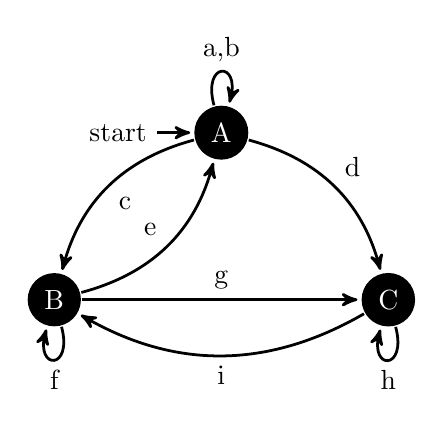
\begin{tikzpicture}[->,>=stealth',shorten >=1pt,auto,node distance=3cm,thick, line width = 1pt]
  \tikzstyle{every state}=[fill=black,draw=none,text=white,minimum size = 0.4cm]

{\node[state,initial]	(A)			{A};}
  
{\node[state]		(B) [below left of=A] 	{B};}
  
{\node[state]		(C) [below right of=A] 	{C};}


\path	(A) edge  [loop above] 	node {a,b} (A)
            edge  [bend right]	node {c} (B)
	    edge  [bend left]	node {d} (C)

        (B) edge [loop below] 	node {f} (B)
	    edge 		node {g} (C)
	    edge [bend right]	node {e} (A)
	
	(C) edge [loop below] 	node {h} (C)
	    edge [bend left] 	node {i} (B)
% 	    edge [bend left]	node {f} (A)
	 ;            
\end{tikzpicture}

%
%\caption{asdfadfs}


\caption{Robot that does a depth-first traversal of binary trees.}
\label{fig:dfs}
%\hfill
%\begin{minipage}[b]{0.45\linewidth}
%    \centering
%    \input{butterfly}
%    \caption{}
%    \label{fig: butterfly}
%\end{minipage}
%
%\begin{minipage}[b]{0.45\linewidth}
%    \centering
%    \input{eye}
%    \caption{}
%    \label{fig: eye}
%\end{minipage}
\end{figure}

% \head{Scheduling}
% Informally, a schedule $\calS$ states which agents are active at every time step.
% We need not think of the schedule as something that a centralised agent produces, but rather as a mathematical way to talk about different timing assumptions, such as synchronous, asychronous, round-robin, etc. In this work we consider asynchronous scheduling, i.e., at every 	
%
% We define typical schedules $\calS$.
%
% Let $c_0, c_1, c_2 \dots$ be a run and let $K_0, K_1, K_2 \dots$ be the active robots at each time step.
%
% The run is \emph{synchronous} if $K_n = [k]$ for every $n$.
%
% The run is \emph{asynchronous} if $|K_n| = 1$ for every $n$.
%
% The run is \emph{fair} if for every $i \leq k$ there are infinitely many $n$ such that $i \in K_n$.
%
% The run is \emph{round-robin} if $K_n = \{n \mod k\}$ for every $n$. Such runs are also fair and asynchronous.
%
% The set of runs following a schedule $\calS$ is denoted $\runs_\calS(G,\tup{R})$.
%
% \todo{formalise the fact that these schedules are definable in MSO}

% \begin{example}
% \todo{give deployment robots example. publish when you move left.}
% \end{example}

\subsection{Robot Linear Temporal Logic (\RLTL) --- a logic of tasks} \label{sec:TL}
%\head{Robot Tasks.} \label{ex:tasks}
%
%: a {\em $k$-robot task}, or simply a {\em task}, $\T$, is a function that maps a graph $G$ to a set of sequences of positions of $G$, i.e.,  $\T(G) \subseteq (V^k)^\omega$. A robot-ensemble $\tup{R}$ {\em achieves} $\T$ on $G$ if for every run $\alpha$ of $\tup{R}$ on $G$ it holds that $\alpha' \in \T(G)$, where $\alpha'$ is the sequence of positions of the run $\alpha$.
%%\sr{should define tasks to be properties of runs? i.e., include states}
%
%\item A robot {\em explores and halts} if, no matter where it starts, it a) eventually halts, and b) visits every vertex of the graph at least once.
%
%\item A robot {\em explores and returns} if, no matter where it starts, it a) eventually halts where it started, and b) visits every vertex of the graph at least once.
%Formally, $v_1 v_2 \cdots \in T(G)$ if and only if there exists $i$ such that $\{v_1,\cdots,v_i\} = V$ and for all $j \geq i$, $v_i = v_j$.
%\sr{but the robot does not know it halts. tasks should also talk about the sequence of states, not just sequence of positions?}
%\item[RT3.] A robot {\em perpetually explores} if, no matter where it starts, it visits every vertex of $G$ infinitely often.
Robots should achieve some task in their environment.
We give some examples of foundational robot tasks \cite{KKR07handbook}:

\it
\- A robot ensemble {\em deploys} or {\em reconfigures} if they move, in a collision-free way, to a certain target configuration.

\- A robot ensemble {\em gathers} if, no matter where each robot starts, there is a vertex $z$, such that eventually every robot is in $z$.

\- A robot ensemble {\em collaboratively explores} a graph if, no matter where they start, every node is eventually visited by at least one robot.

\- All of these tasks have {\em safe} variations: the robots complete their task without entering certain pre-designated ``bad'' nodes of the graph.

\ti


%
%\item[RT4.] An ensemble of robots {\em catches} a single robot if no matter where they start, at some point in time one robot in the ensemble is in the same vertex as the single robot. Note that unlike the previous examples, this task is adversarial.
% A robot {\em explores} if, no matter where it starts, it eventually visits every vertex of the graph at least once.


%no space
%Note that there are some natural relations between these tasks. If robots can explore and return, then in particular they can explore and halt. If they can explore and halt, then they can perpetually explore. If they can perpetually explore then, using the fact that they have IDs, they can gather --- every robot searches for the robot with the smallest ID, which stays still (with two agents this is called ``wait for mommy'').


%
We now define \RLTL, a logic for formally expressing tasks from the robots' points of view. The idea is that \RLTL is \LTL in which the atoms are tests.

% The syntax is \LTL over the alphabet of tests.
% The models of \RLTL are sequences of configurations. The semantics $\models_i$ (for $i \leq k$) of \RLTL are given as in \LTL, where the atomic case is
% ``robot $i$ satisfies test $\tau$ at the current configuration''. Finally, we interpret \RLTL over models of the form $\activeproj_i(\pi)$ where $i \leq k$ and $\pi \in \runs(G,\tup{R})$.


{\bf Syntax.} Let $k \in \nat$ and $\Sigma$ be a set of edge-labels.
Formulas of $\RLTL_k(\Sigma)$ are those of $\LTL(\uptau_k(\Sigma))$ where $\uptau_k(\Sigma)$ is the set of tests for $k$ robots on $\Sigma$-labeled graphs.
If $k$ and $\Sigma$ are understood from the context, we write $\RLTL$ instead of $\RLTL_k(\Sigma)$.

{\bf Semantics.} Fix $i \leq k$. For a sequence of configurations $\alpha = c_0 c_1 \cdots$ and an $\RLTL_k(\Sigma)$ formula $\varphi$, write
$\alpha \models_i \varphi$ if $\alpha$ satisfies $\varphi$ as an \LTL formula whose atoms are tests interpreted wrt robot $i$.
Formally, for formula $\varphi$ and $n \geq 0$, define $(\alpha,n) \models_i \varphi$ inductively (all cases are like \LTL, the only difference is
the first item, i.e., the atomic case):
	\it
	\- $(\alpha,n) \models_i \tau$ iff $Sat(\alpha_n,\tau,i)$ (i.e., robot $i$ satisfies test $\tau$ in $\alpha_n$);
	\- $(\alpha,n) \models_i \varphi_1 \wedge \varphi_2$ iff $(\alpha,n) \models \varphi_j$ for $j = 1,2$;
	\-	$(\alpha,n) \models_i \neg \varphi$ iff it is not the case that $(\alpha,n) \models \varphi$;
	\-  $(\alpha,n) \models_i \nextX \varphi$ iff $(\alpha,n+1) \models \varphi$;
	\- $(\alpha,n) \models_i \varphi_1 \until \varphi_2$ iff there exists $j \geq n$ such that $(\alpha,j) \models_i \varphi_2$ and for all $l \leq j < n$, $(\alpha,l) \models_i \varphi_1$.
	\ti
	Write $\alpha \models_i \varphi$ if $(\alpha,0) \models_i \varphi$.

For a $\Sigma$-graph $G$ and a $k$-robot ensemble $\tup{R}$, write $(G,\tup{R}) \models_i \varphi$ if for all $\pi \in \runs(G,\tup{R})$,
it holds that $\activeproj_i(\pi) \models_i \varphi$. We say that \emph{Robot $i$ satisfies $\varphi$}.
Finally, given \RLTL formulas $\varphi_i$ for each robot $i \in [k]$, write $(G,\tup{R}) \models \tpl{\varphi_1,\cdots,\varphi_k}$ if $(G,\tup{R}) \models_i \varphi_i$ for all $i \in [k]$.



%To express that some run satisfies $\varphi$, we could write $(G,\tup{R}) \not \models \neg \varphi$.

%Thus, given a graph $G$ and $k$-ensemble of robots $\tup{R}$ where the $i$th robot $R_i$ has state set $Q_i$, initial-state set $I_i$,
%% repeating-state set $A$,
%and halting-state set $H_i$, accepting-state set $A_i$,

\begin{example}[avoid halting state]
The \RLTL safety formula $\always  (st_{cur} \not \in H)$ says that the last published state of the robot is never in the set $H$.
\end{example}

\begin{example}[gather]
The \RLTL formula 
\[ \eventually\left[ (\bigwedge_j \VARpos_{cur} = \VARbcpos_j) \wedge \always (\VARpos_{cur} = \nextX \VARpos_{cur})\right] 
\]
 states that eventually
the current position of the robot is equal to the last published position of all the robots (including itself), and that from that point on the robot never moves.
In words, every robot satisfies this formula if and only if the robots gather (and do not disperse) at a vertex of the graph at which they last published. %sent their last broadcast.
\end{example}
%The \RLTL safety formula $\always \textsc{diff}$ where $\textsc{diff} := \bigwedge_{i \neq j} x_i \neq x_j$ says that it is always the case that the published positions of different robots do not agree. Thus, if a robot broadcasts its position whenever it moves, then this formula says that the robots never collide.

\begin{example}[deploy to leaves] \label{ex:RLTL-deploy}
 Suppose $G$ is a tree and let $\isleaf(z)$ be the test that says that position $z$ is a leaf in the tree.
%  , e.g., for binary trees,
%  $\isleaf(z) = \neg \exists x.\lambda(z,x) = lc \vee \lambda(z,x) = rc$.
 Let $\mathit{diff}$ be the formula $\bigwedge_{i \neq j} pos_i \neq pos_j$.
The \RLTL formula $\mathit{diff} \limp\left[\eventually \isleaf(\VARpos_{cur}) \wedge \always(\bigwedge_{j\neq i} \VARpos_{cur} \neq pos_j)\right]$
states that if the robots begin in different vertices of the tree $G$, then
eventually the robot reaches a leaf, and it is never in the same position as a published position of another robot.
In words, every robot satisfies this formula if and only if, assuming robots begin at different vertices of the tree $G$, the robots deploy to the leaves while not colliding with the last published positions of any other robot.
%
% In words, every robot satisfies this formula if and only if, assuming robots begin at different vertices of the tree $G$, the robots deploy to the leaves while not colliding with any other robot (according to published positions).
%
\end{example}

In order to define collaborative exploration, we will need an extension of our logic to allow tests over the accumulated positions, see Section~\ref{sec:extensions}.


%\item The $\msol$-formula $\forall \tup{x} \exists \tup{y} \exists \tup{X}. \bigcup X_i = V \wedge \psi_\alpha(\tup{X},\tup{x},\tup{y})$ says that, no matter where they start, there is a run according to a schedule that follows $\alpha$ in which the robots collaboratively explore the graph.

%\item The $\msol$-formula (to be interpreted on trees)
%where $\textsc{nonleaf}(\tup{x})$ is an $\msol$-formula expressing that every $x_i$ is not a leaf, $\textsc{leaf}(\tup{y})$ expresses that every $y_i$ is a leaf, and $\textsc{diff}(\tup{z})$ expresses that $z_i \neq z_j$ for $i \neq j$. On trees this formula expresses that for every ordering $\alpha$ of processes that switch $N$-times, there is a run according to a schedule that follows $\alpha$ such that the robots reconfigure from different internal nodes to different internal leaves.\footnote{If one wants to add that the paths of the robots are collision-free one can replace $Reach$, for the case of two robots in which robot $1$ moves and then robot $2$ moves (for instance), by the formula
%$\exists \tup{Z} \exists \tup{Y} \exists \tup{z}\left[ \psi_1(\tup{Z},\tup{x},\tup{z}) \wedge \psi_2(\tup{Y},\tup{z},\tup{y})
%  \wedge Z_1 \cap Y_2 = \emptyset \right]
%$.}

% expresses, on trees, that no matter which internal nodes of the tree two robots start on, they have a collision-free path ($Z_1 \cap Y_2 = \emptyset$) in which they reach different leaves, according to a schedule in which robot $1$ is scheduled and then robot $2$ is scheduled. Similar more complex formulas can express the reconfiguration task of Example \ref{ex:recon} for (collaborative or adversarial) $b$-switching schedules.
%\item The atomic formula $Infty(X,x,y)$ expresses that the robot, starting in position $x$, visits position $y$ infinitely often, and the set of vertices the robot visits along this run is exactly $X$. Thus $\forall x Infty(V,x,x)$ is an \RLTL\ formula expressing that the robot ``perpetually explores'' the graph.

%\item The \RLTL\ formula $\exists \tup{x} \exists \tup{X} [Halt(\tup{X},\tup{x},\tup{x}) \wedge \cup_i X_i = V ]$, which talks about $k$ robots, expresses that each robot eventually returns and halts in its starting position, and every vertex of the graph is visited by at least one of the robots.


%\item The atomic formula $Infty(X,x,y)$ expresses that the robot, starting in position $x$, visits position $y$ infinitely often, and the set of vertices the robot visits along this run is exactly $X$. Thus $\forall x Infty(V,x,x)$ is an \RLTL\ formula expressing that the robot ``perpetually explores'' the graph.

%\item The \RLTL\ formula $\exists \tup{x} \exists \tup{X} [Halt(\tup{X},\tup{x},\tup{x}) \wedge \cup_i X_i = V ]$, which talks about $k$ robots, expresses that each robot eventually returns and halts in its starting position, and every vertex of the graph is visited by at least one of the robots.

%if $k=1$ and Lemma~\ref{lem:kcompile} if $k > 1$;
%$Q := \prod_{i \in [k]} Q_i$ is the set of tuples of states, $I := \prod_{i \in [k]} I_i$ is the set of tuples of initial states, $A := \prod_{i \in [k]} A_i$ are the repeating tuples, and $H := \prod_{i\leq k} H_i$ are the halting tuples.  We will often supress mention of $k$ and write, for instance, $Reach(\tup{X},\tup{x},\tup{y})$.

%an execution $\alpha \in (V^k \times \prod_{i \in [k]} Q_i)^*$ with $\alpha_1$ an initial configuration suppose $I_i \subseteq Q_i$ are the initial states, $A_i \subseteq Q_i$ are the accepting states, and $H_i \subseteq Q_i$ are the halting states:
%$(G,\tup{R}) \models Reach(\tup{x},\tup{y})$ iff there exists a  &\textrm{ iff } \alpha_1 = (\tup{q},\tup{x}) \textrm{ is initial, and } \exists i \in \nat\, \alpha_i = \tup{y}$


% such and every $k$-robot ensemble $\tup{R} = \tpl{R_1,\cdots,R_k}$, and all $k$-tuples of states $\tup{q},\tup{s} \in \prod_{i \in [k]} Q_i$, there is an atomic formula $\tup{R}_{\tup{p},\tup{q}}$  (of arity $2k$) where $\tup{R}_{\tup{p},\tup{q}}(\tup{x},\tup{y})$ expresses that there is an execution of the ensemble $\tup{R}$ starting with configuration $\tpl{\tup{x},\tup{p}}$ and containing\sr{ending?} the configuration $\tpl{\tup{y},\tup{q}}$.


%Formulas written in MSOL can quantify over sets (of vertices and edges). Thus they can express graph properties such as whether the graph is connected, whether it has  a $k$-colouring, whether it is planar, but not whether it is rigid.\sr{are these relevant properties?}

%A cornerstone of automata theory states that MSOL over finite/infinite words/trees coincides with automata operating on finite/infinite words/trees \cite{}.
%MSOL


\section{Parameterised Verification of Robot Systems}

In this short section, we formalise the parameterised verification problem (PVP) for robot protocols and provide the basic tools which allows one to prove undecidability of certain classes of PVP problems. We illustrate with a simple undecidability result that says that PVP is undecidable, even for a single robot, on grids. In the following two sections we provide deeper undecidability and decidability results.
%, show that it is undecidable already in some very restricted cases, and then describe a simple restriction on the orderings, namely bounded switching, that guarantees decidability, which we show by reducing to the validity problem of certain logics.
%
%\head{The Parameterised Verification Problem.}

% Fix a set of $\Sigma$-graphs $\gclass$.
% \begin{definition}
% The \textbf{parameterised verification problem} $\PVP(\gclass)$ is: given a number $k \in \nat$ of robots, a $k$-robot ensemble $\tup{R}$, and an \RLTL formula $\T$, decide whether for every graph $G \in \gclass$, $(G,\tup{R}) \models \T$.
% \end{definition}
\begin{definition}
Fix a set of $\Sigma$-graphs $\gclass$, positive integer $k$, a set  $\rclass$ of $k$-robot ensembles, and a set $\tclass$ of $\RLTL_k(\Sigma)$ formulas.
The \textbf{parameterised verification problem} $\PVP(\gclass,k,\rclass,\tclass)$ is the following decision problem: given a $k$-robot ensemble $\tup{R} \in \rclass$, and a $k$-tuple of \RLTL formulas $\tpl{\varphi_1,\cdots,\varphi_k}$ from $\tclass$, decide whether for every graph $G \in \gclass$ it holds that $(G,\tup{R}) \models \tpl{\varphi_1,\cdots,\varphi_k}$, i.e., whether for every $G \in \gclass$ every robot $i$ satisfies $\varphi_i$.
\end{definition}

% \emph{Notation.}
% \it
% \- In case $\tclass$ consists of a single formula $\T$ we write $\PVP(\gclass,k,\rclass,\T)$ instead.
%
% % \- We may write $\PVP$ instead of $\PVP(\gclass,k,\rclass,\tclass)$ to ease the reading.
% \ti


% \begin{example} \sr{ordering}
% Let $\gclass$ be the set of all binary trees, $\rclass$ be the set of all $k$-robot ensembles,  let $\Omega_b := \{\alpha \in [k]^* : ||\alpha|| = b\}$ be the set of {\em $b$-switch orderings}, and let $T$ be the task expressing that if the robots start on different internal nodes of a tree then they eventually reconfigure themselves to be on different leaves of the tree, no matter which ordering from $\Omega_b$ is chosen (cf. Example~\ref{ex:formulas}). We will see later that one can decide $\PVP_{\T,\Omega_b}(\gclass,\rclass)$ given $b \in \nat$. So, one can decide, given $b$, whether the protocol from the reconfiguration example (in the Introduction) succeeds for every ordering with $b$ switches.
% \end{example}

We now introduce two-counter machines, a Turing-complete model of computation that will be used in the undecidability proofs.




\subsection{Two-counter machines}
An \emph{input-free two-counter machine} (2CM)~\cite{Minsky67} is a deterministic program manipulating two non-negative integer counters, called Counter $1$ and Counter $2$, both initialised to zero, using commands that can increment a given counter by $1$, decrement a given counter by $1$ (if the counter is not zero), and branch depending on whether or not a given counter is equal to zero. We refer to the ``line numbers'' of the program code as the ``states'' of the machine.

\begin{definition}[2CM]
A 2CM is a tuple $M = (Q,q_0,h,C)$ where $Q = [m]$ is a finite set of numbered \emph{states} ($m \in \nat$), $q_0 \in Q$ is the \emph{initial state}, 
$h \in Q$ is the \emph{halting state}, and
$C$ is a function associating each state $q \in Q$ to a \emph{command} which is an expression of the form ``increment counter $i$ and goto state $q+1$'', ``decrement counter $i$ and goto state $q+1$'', and ``if counter $i$ is zero goto $q'$ else goto $q''$'' where $i = 1,2$ and $q',q'' \in L$.
\end{definition}

We assume that every command ``decrement counter $i$'' is guarded by a command that tests that counter $i$ is not zero.
A \emph{configuration of $M$} is a triple $(q,c_1,c_2) \in Q \times \nat \times \nat$. The \emph{initial configuration} of $M$ is $(q_0,0,0)$ and the \emph{halting configurations} of $M$ are $\{h\} \times \nat \times \nat$.  Given a configuration $(q,c_1,c_2)$ there is at most one \emph{successive configuration}, i.e., if the command at $q$ is ``increment counter $1$'' then the successive configuration is $(q+1,c_1+1,c_2)$, if it is ``decrement counter $1$'' then it is $(q+1,c_1-1,c_2)$, if it is ``if counter $1$ is zero goto $q'$ else goto $q''$`` then it is $(q',c_1,c_2)$ if $c_1 = 0$ and $(q'',c_1,c_2)$ otherwise, and similar definitions hold for counter $2$. Thus, there is a unique maximal (possibly finite) sequence that starts in the initial configuration and stops once, if at all, a halting configuration is reached. This is called the \emph{computation} of the 2CM. We say that the 2CM \emph{halts} if the computation is finite and ends in a halting configuration.
% Observe that if the computation is finite then the values of both counters are bounded by some integer $n$. 
The \emph{non-halting problem for 2CMs} is to decide, given a 2CM $\cm$, whether it does not halt. This problem is undecidable (cf. \cite{Minsky67}), and is usually a convenient choice for proving undecidability of problems concerning parameterised systems due to the simplicity of the operations of counter machines~\cite{Emerso03,AJKR14,DBLP:conf/cade/AminofR16}.

\subsection{Basic undecidability result}
To show undecidability we reduce the non-halting problem of two-counter machines to certain parameterised verification problems.

That is, given a 2CM machine $M$, we build robot(s) $\tup{R}$ and a tuple of formulas $\tpl{\varphi_1,\cdots,\varphi_k}$
such that the run of $M$ never reaches a halting state if and only if
$(G,\tup{R}) \models \tpl{\varphi_1,\cdots,\varphi_k}$ for all $G \in \gclass$. We illustrate with a basic undecidability result on grids that states that
PVP is undecidable already for a single robot on grids with simple testing abilities and a safety task.
The proof ideas were already observed in \cite{BlHe67} for a different setting.
% for ``2-dimensional automata''.


\begin{theorem}[Grid, boundary testing] \label{thm:undec-1robotgrid}
$\PVP(\gclass,k,\rclass,\tclass)$ is undecidable for the following data:
\it
\- $\gclass = \{G_n : n \in \nat\}$ is the set of grids (so $\Sigma = \{u,d,l,r\}$),
\- $k = 1$,
\- $\rclass$ is the set of $1$-robot ensembles, with no publishing states, that can test whether or not they are on a given boundary of the grid,
\- $\tclass$ consists of the single safety formula $\always (st_{cur}  \neq h)$.
\ti
\end{theorem}



% \todo{- add to statement of thm that robots don't need publishing states.}

% \todo{- fix initial states. either put them in the formula, or in the graph.}
\begin{proof}
 The idea is that counter values $(n,m) \in \nat^2$ are encoded by the robot being at position $(n,m)$ of the grid, and the only tests that are needed are to check whether or not the robot is on a given boundary. Indeed, given a 2CM $\cm$, the robot $R_\cm$ stores the current state of $\cm$. If the current state is $q$ and the current command is ``increment (resp. decrement) counter $1$'' then the robot tests if it is on the right (resp. left) boundary, and if not it moves one step to the right (resp. left) and updates its state to $q+1$, and if yes it enters a failure sink state $\bot$. ``Increment (resp. decrement) counter $2$'' is similar, and involves moving up (resp. down) and entering the failure sink $\bot$ if the tests fail. Finally ``test counter $1$ (resp. $2$) for zero'' is done by testing if the robot is on the left (resp. bottom) boundary. Before the robot starts the simulation, it moves to co-ordinate $(0,0)$ (which it can do since it can test for boundaries). Note that for every $n$ the set $\runs(G_n,R_\cm)$ contains a single run. Moreover, the run of $\cm$ never halts iff for every $n$ the run in $\runs(G_n,R_\cm)$ never reaches the halting state. \qed
\end{proof}

This theorem strongly suggests that one cannot get decidable PVP unless one limits at least one of the following: the testing abilities of the robots, the moving abilities of the robots, or the class of graphs. The above undecidability result for grids made use of only a single robot with very basic testing abilities (i.e., boundary detection). Thus, there is not much hope for an interesting model if we further restrict the testing abilities. Limiting the movement of robots on grids was studied in \cite{AAMAS16Grids}. There, one disallows robots from specifying their exact positions in the grid, e.g., a robot may decide to move to the left but not specify the exact number of steps. In the present work, instead, we consider robots with powerful remote-testing and the ability to specify their movements exactly. We restrict the set of graphs that are definable in monadic second-order logic and of bounded clique-width. We call these \courcellian sets of graphs. These do not include grids, but do include, e.g., lines, trees, and cliques, see section~\ref{sec:dec}.
% As we will see in Section~\ref{sec:DEC k=1} this restriction on the sets of graphs is enough to get decidable PVP for systems consisting of only a single robot.
However, this restriction on its own is not enough.
In the next section, we give undecidability results for multiple robots and possibly the simplest sets of \courcellian graphs, i.e.,
lines (thus indicating that further restricting the graphs will not yield interesting models).
The undecidability results imply that one has to impose limitations on their
``communications'' in order to regain decidability for multiple robots.
Specifically, the limitation on the robots state that there
is a bound on the number of times that a robot can test another robot's current
state and position, and a similar limitation must
be imposed on the specification logic.
%Interestingly enough, these restrictions are neccessary even if one limits robots to very basic tests (i.e., collision detection).

% \ba{Update rest of this section.}
%
%
% In the next section it is shown that the PVP is undecidable for two synchronous robots on a line, and very simple tasks. In light of this negative result, we explore in what ways we can restrict the robots to gain decidability. One possible direction is to limit the sensing/communication between the robots. Indeed, the above mentioned undecidability result assumes that each robot can sense/query whether the other robot is at the left-most position of the line. Another possibility is to consider the case of asynchronous robots. In Section \ref{sec:PVPundec} we show that the assumption of asynchronous robots alone does not guarantee decidability of the parameterised verification problem already in the very restricted case of reachability tasks on lines. Interestingly enough, our proof also applies \todo{check} to the synchronous case,  and assumes only very limited sensing capabilities, namely, that a robot can sense which of the other robots shares the same position with it (i.e., ``collision detection''). This fact strongly suggests that limiting the robots' sensing capabilities may not be a very fruitful direction. In Section \ref{sec:PVPdec} we show that for asynchronous robots with full testing abilities we can guarantee decidability by i) restricting to context-free environments, and ii) restricting to $B$-broadcast schedules. As we have just seen, dropping either of these two restrictions results in undecidability.



\section{Undecidability of Multi-Robot Systems on Lines} \label{sec:PVPundec}

In this section we deal with multiple robots on lines.

We describe the \emph{basic encoding} that translates a 2CM $\cm$ into a robot ensemble $\tup{R}$ which, on longer and longer lines, can simulate longer and longer prefixes of the computation of $\cm$ (and thus, if $\cm$ halts, can simulate the entire computation of $\cm$ on a long enough line).
We use two \emph{counter} robots $\counter_1$ and $\counter_2$. The current position of $\counter_i$ on the line corresponds to the current value of counter $i$, and it moves to the right to increment counter $i$ and to the left to decrement it.
Each of these robots also stores in its finite memory the current state of the 2CM.
If a robot can't successfully execute a command (e.g., the command is to increment but the robot is already at the right end-point of the line), then the robot enters a special failure sink $\bot$. The basic difficulty is to ensure that the counter robots stay synchronised, e.g., if $C_1$ simulates a test counter $1$ for zero, then $C_2$ should learn the result of that test before the simulation continues.

\head{Notation.} We use the following position tests. Let $RE(x) := \neg \exists y. \lambda(x,y) = r$ be the test that checks if $x$ is at the right end-point of the line, 
and let $LE(x) := \neg \exists y. \lambda(x,y) = l$ be the test that checks if $x$ is at the left end-point of the line.

We begin with a striking result that shows the power of the task logic \RLTL. It says that PVP is undecidable for robots with \emph{no testing abilities}. A robot will guess whether it is on a given end-point of the line. The \RLTL formula itself is used to filter out the runs in which the robot makes incorrect guesses. To do this, we require that robots publish their position from every state.


% RETURN COMMENT IN PUBLISHED VERSION
% \todo{B: why do we need this footnote at this stage?}
% \footnote{A similar proof idea, in a different setting, can be found in \cite{Igoretc} which shows that parameterised model checking of distributed systems that don't communicate is undecidable for formulas of (non-prenex) indexed-\LTL.}

\begin{theorem}[Lines, no testing] \label{thm:undec-lines-no testing}
$\PVP(\gclass,k,\rclass,\tclass)$ is undecidable for the following data:
\it
\- $\gclass = \{L_n : n \in \nat\}$ is the set of lines (so $\Sigma = \{l,r\}$),
\- $k = 2$,
\- $\rclass$ is the set of $2$-robot ensembles with no testing abilities, and for which every state is a publishing state,
\- $\tclass$ consists of all \RLTL formulas.
% $\varphi$ (defined later). \sr{not single}
\ti
\end{theorem}

% % \todo{- fix formulas. their should be one for each robot.}


\begin{proof}
As in the basic encoding, the position of Robot $i$ on the line encodes the current value of Counter $i$. Since the robot has no testing abilities, it cannot test whether it (or the other robot) has successfully executed a
command of the 2CM. Instead, the robots nondeterministically guess the answer to the relevant boundary test, and the formula $\phi$ (of Robot $1$, say) will filter out those runs in which the guesses are incorrect. Moreover, the formula $\phi$ ensures that both robots stay synchronised, i.e., they always store the same state of the 2CM.
% The formula of Robot $2$ can be taken to be $\true$.

Formally, fix a 2CM $(Q,q_0,h,C)$. The states (and publishing states) of each robot are $Q \cup \{\bot\}$ and the only initial state of each robot is $q_0$.  
We now describe the transitions. First, $\bot$ is a sink state, i.e., $(\bot,\gc{\true}{stay},\bot)$ is a transition. Let $Inc_1$ be the set of states of the 2CM whose command is of the form ``increment counter $1$''. For each $q \in Inc_1$,
robot $1$ has transitions $(q,\gc{\true}{r},q+1)$ and $(q,\gc{\true}{stay},\bot)$, and
robot $2$ has transitions $(q,\gc{\true}{stay},q+1)$ and $(q,\gc{\true}{stay},\bot)$. Transitions for the other commands are similar. Let $R_1,R_2$ be the constructed robots.

Define an \RLTL formula $\psi_{simulate}$ to be the conjunction of 6 formulas, one for each type of command of the 2CM. E.g., the command ``increment counter $2$'' is coded by the formula 
\begin{align*}
 \bigwedge_{q \in Inc_2} & st_2 = q  \limp \\
 & \left[(\neg RE(\VARbcpos_2) \limp \nextX(st_2 = q+1)) \wedge (RE(\VARbcpos_2) \limp \nextX(st_2 = \bot))\right].
\end{align*}
Similarly, the command ``if counter $1$ is zero goto $q'$ else goto $q''$'' is coded by the formula
\begin{align*}
 \bigwedge_{(q,q',q'') \in Test_1} & st_1 = q \limp \\
 & \left[(LE(\VARbcpos_1) \limp \nextX(st_1 = q')) \wedge (\neg LE(\VARbcpos_1) \limp \nextX(st_1 = q''))\right]
\end{align*}
where $Test_1$ is the set of triples $(q,q',q'')$ such that the command of the 2CM at line $q$ is ``if counter $1$ is zero goto $q'$ else goto $q''$.



Then, it is easy to see that the 2CM machine halts (on its unique computation) if and only if there is a line and a run $\pi$ of the two robots $\tup{R} = R_1,R_2$ on this line such that $\activeproj_1(\pi)$ satisfies the \RLTL formula $\varphi$ defined by $(\VARbcpos_1 = \VARbcpos_2 = 0) \wedge \always (st_1 = st_2) \wedge \eventually (st_1  = h) \wedge \always \psi_{simulate}$. Thus, the 2CM does not halt iff for every line $G$, it holds that $(G,\tup{R}) \models \tpl{\neg \varphi,\true}$.
\qed
\end{proof}

% \todo{-there might be a stupid technicality to take care of: what if a branching command from line l says to branch back to l? B: we can assume no such commands w.l.o.g.}

% \todo{-again, take care of initial state}

%Indeed, suppose the 2CM halts, and let $N$ be the largest value of any of the counters. Then it is easy to see that there is a run of the robots on the line of length $N$ satisfying $\always(st_1 = st_2)$ and $\eventually(st_1 = h)$. Conversely, suppose there is a run of the robots on some line, say of length $N$, satisfying $\always (st_1 = st_2)$ and $\eventually (st_1  = h)$. By the first formula, the robots are always in the same state. Thus, if one changes state, the other simultaneously changes to the same state. By construction, the transitions of the robots ensure that each faithfully simulates the 2CM.


\begin{remark}
Looking at the proof we see that we don't need all \RLTL formulas: it is enough to restrict to, e.g., \RLTL formulas without $\until$, without nesting $\nextX$, and whose atoms are state-tests (that may compare the states of both robots with each other) and position-tests for the left and right end-points of the line.
\end{remark}

\begin{remark}
If we had defined the semantics of \RLTL over runs $\pi \in \runs(G,\tup{R})$ directly (instead of over $\activeproj_i(\pi)$) and allowed formulas to \emph{simultaneously} talk about the \emph{current} positions and states of all robots, then the same proof would would give us undecidability for robots
with no testing abilities and \emph{no publishing states}. 
\end{remark}


% The previous theorem shows that to get decidability we must either restrict the publishing abilities of the robots, or the \RLTL formulas under consideration. In the rest of this section we show that even for simple safety \RLTL formulas, and increasingly elementary robot testing abilities, PVP is undecidable if the publishing abilities are not restricted.

 The previous theorem shows that, even if robots do not have any access to information regarding the states or positions of other robots, in order to get decidability we must not allow the specification formula of one robot to access exact up-to-date information about the states and positions of the other robots. Symmetrically, the following theorem shows that, even if the specification formula of each robot does not have any access to information regarding the states or positions of other robots (actually, even without access to the position of the robot itself), in order to get decidability we must not allow one robot to have exact up-to-date information about the states and positions of the other robots.


% 
% \begin{theorem}[Lines, Remote Testing] \label{thm:undec-synchline}
% $\PVP(\gclass,k,\rclass,\tclass)$ is undecidable for the following data:
% \it
% \- $\gclass = \{L_n : n \in \nat\}$ is the set of lines (so $\Sigma = \{l,r\}$),
% \- $k = 2$,
% \- $\rclass$ is the set of $2$-robot ensembles in which a) each robot is able to test the other robot's state, b) robots are able to test if they, or the other robot, is at the left (resp. right) end of the line, c) every state is a publishing state,
% \- $\tclass$ consists of a single \RLTL safety formula (defined later). 
% \ti
% \end{theorem}
%\sr{robots can be taken deterministic}


\begin{theorem}[Lines, Remote Testing] \label{thm:undec-synchline}
$\PVP(\gclass,k,\rclass,\tclass)$ is undecidable for the following data:
\it
\- $\gclass = \{L_n : n \in \nat\}$ is the set of lines (so $\Sigma = \{l,r\}$),
\- $k = 2$,
\- $\rclass$ is the set of $2$-robot ensembles in which a) each robot is able to test the other robot's state, b) each robot is able to test if it, or the other robot, is at the left (resp. right) end-point of the line, and 
c) every state is a publishing state,
\- $\tclass$ consists of a single \RLTL safety formula that only talks about the current state of the robot (and not about positions or about published states).
\ti
\end{theorem}
\begin{proof}
Before describing the reduction, we describe how to enforce that the robots are scheduled round-robin (note that the task formula is too simple to enforce this).
The robots' states include a special variable that cycles through the values in $\{1,2\}$. Let $a_i$ be the value of this variable for robot $i$ at a given point in time. At the beginning $a_i = i$. Robot $i$'s guarded-commands that simulate the 2CM (see below) are guarded by the test $a_1 + a_2$ is congruent to $i$ modulo $2$, and after executing the 
robot $i$ switches the value of its variable. 
% that says that $a_i + a_{3-i}$ is equal to $1$ modulo $3$ (e.g., if $a_i = 0$ then the instruction includes the guard $a_{3-i} = 2$). Suppose $a_1 \neq a_2$. Then i) exactly one robot has a true guard, and ii) after that robot updates its variable, $a_1 \neq a_2$.
% %; if $a_i = 1$ then the instruction includes the guard $a_{3-i} = 0$; and if $a_i = 2$ then the instruction includes the guard $a_{3-i} = 1$.
% The robots begin with $a_1 = 0$ and $a_2 = 2$, and thus by i) and ii), the robots alternate round-robin. To spell things out,
% at the beginning only robot $1$ has an enabled guard, after which $a_1 = 1, a_2 = 2$. Then, only robot $2$ has an enabled guard, after which $a_1 = 1, a_2 = 0$, etc.
% This yields the following $(a_1,a_2)$-sequence $((0,2) (1,2) (1,0) (2,0) (2,1) (0,1))^\omega$, which corresponds to the robots alternating turns at every time step, starting with robot $1$. 
Thus, the $(a_1,a_2)$-sequence evolves as follows: $(1,2) (2,2) (2,1) (1,1) (1,2) \dots$. 
This completes the description of the mechanism that enforces round-robin. Note that this mechanism uses the ability of robots to
perform remote state-tests and that every state is a publishing state. 

Given a 2CM $\cm$ with state set $Q$, the states of the robots are of the form $(a,q) \in \{1,2\} \times (Q \cup \{\bot\})$. 
Formalise the tests ensuring round-robin as follows: for $i = 1,2$, write $T_i = \{i\} \times (Q \cup \{\bot\})$, and 
define $\tau_i$ to be $\bigvee st_1 \in T_x \wedge st_2 \in T_y$ where the disjunction is over pairs $(x,y)$ such that $x+y = i \mod 2$.

If $l = \bot$ then robot $i$ has transitions from $(a,q)$ to $(a,q)$ with guarded-command $\gc{\tau_i}{stay}$, i.e., a sink.  

The robots running on $L_n$ simulate a command of $\cm$ as follows. We describe increments (decrements are similar), and tests for zero.
Suppose $q \in Q$ and the command of the 2CM at state $q$ is ``increment counter $3-i$''. Then robot $i$ has the transition from $(a,q)$ to $(3-a,q+1)$ with guarded-command $\gc{\tau_i}{stay}$. Similarly, if the command at state $q$ is ``increment counter $i$'' then robot $i$ has the transition from $(a,q)$ to $(3-a,q+1)$ with guarded-command $\gc{\tau_i \wedge \neg RE(\VARpos_{cur})}{move(r)}$, and it has the transition from $(a,q)$ to $(3-a,\bot)$ with guarded-command $\gc{\tau_i \wedge RE(\VARpos_{cur})}{stay}$. 
% Here $RE(cur)$ is the test $\neg \exists y. \lambda(cur,y) = r$.


Suppose $q \in Q$ and the command at state $q$ is ``if counter $j$ is zero goto state $q'$ else goto $q''$''. Then robot $i$ has the transition from $(a,q)$ to $(3-a,q')$ with guarded-command $\gc{\tau_i \wedge LE(\VARbcpos_j)}{stay}$, and a transition from $(a,q)$ to $(3-a,q'')$ with guarded-command $\gc{\tau_i \wedge \neg LE(\VARbcpos_j)}{stay}$. 
% Here $LE(pos_j)$ is the test $\neg \exists y. \lambda(y,pos_j) = r$.

Define $H = \{1,2\} \times \{h\}$ where $h$ is the halting state of the 2CM. Define $\Phi$ to be the formula $\eventually (st_{cur} \in H)$.
It is not hard to see that 2CM halts iff there exists $n \in \nat$, a run $\pi$ of the robots on $L_n$, and an $i = 1,2$ such that $active_i(\pi) \models \Phi$. Thus, the 2CM does not halt iff for every line $G$, it holds that $(G,\tup{R}) \models \tpl{\neg \Phi,\neg \Phi}$. \qed
% for all $n \in \nat$ and $i = 1,2$, for all runs of the robots on $L_n$, it is never the case that the current state of robot $i$ is in $H$. \qed
\end{proof}





% Robot $i$ has a variable variable $l_i$
% Each robot stores what it considers to be the current state $l$ of the 2CM. Suppose the command at state $l$ is ``increment counter $i$''. 
% Consider robot $i$. If the command of its current line-number $l$ is ``increment counter $i$'' (i.e., increment the counter that it represents) then: if it is not at the right end-point, it moves one step to the right and changes its line-number to $l+1$, and if it is on the right end-point it enters a failure sink $\bot$. On the other hand, if the command of its current line-number $l$ is ``increment counter $3-i$'' (i.e., increment the other counter) then robot $i$ copies the state of robot $3-i$ (more precisely, it tests the state $s$ of robot $3-i$: if $s$ stores line-number $l$ then robot $i$ does not change its line-number, although it will fire the transition ensuring round-robin; if $s$ stores the line-number $l+1$ then robot $i$ changes its line-number to $l+1$; if $s = \bot$ then robot $i$ itself changes its state to $\bot$). The other commands, ``decrement counter $i$'' and ``test counter $i$ for zero'' are defined similarly. 

% 
% For a given 2CM $\cm$ we build a pair of robots $R_M$. First, each robot moves to the left end-point of the line. Then, the robots begin simulating \cm. Each robot stores the current state of \cm. However, since robots have remote tests, they can correctly simulate all 2CM commands. E.g., to simulate the 2CM command ``increment counter $1$'', robot $i$ tests if robot $1$ is at the right end-point of the line: if ``yes'', then robot $i$ enters a fail state $\bot$; and if ``no'' then robot $1$ moves one position to the right and updates the state of the 2CM being simulated, and robot $2$ updates the state of the 2CM being simulated. Thus, every run $\pi \in \runs(L_n,R_M)$ satisfies 
% $\always (st_1 = st_2 \wedge st_1 \neq h)$ (where $h$ is a halting state of the 2CM $M$) iff the run of $\cm$ never halts.
% \qed

% 
% \begin{remark}
% A similar result was stated in \cite{Rubin15AAMAS} in which it was assumed that robots are scheduled synchronously.
% An alternative proof (of this fact about synchronous robots) is to directly code computations of Turing machines, as was done by~\cite{Ro66} for showing that universality of $2$-head one-way finite-state automata is undecidable.
% \end{remark}


%given a turing machine $M$, build a robot $R_M$ that runs on a grid and checks whether or not the labelings of each row are $M$-configurations that form, in sequence, an accepting run of $M$; if not, then let $R_M$ halt, and otherwise let it run forever. Then $M$ has no accepting run if and only if $R_M$ achieves $T$ on all graphs $G \in \gclass$.

Note that the robots in these proofs have remote sensing abilities, i.e., they can test the positions %/states 
of other robots, no matter where those robots are.
We now consider the case that the robots only have \emph{local} sensing abilities. We allow a robot to test
if it is at the right end-point of the line, and to test which of the other robots are in the same node as it is (``collision detection''). 
Note that a robot cannot test that another robot has collided with it unless the other robot publishes its position. Thus, for this proof, we assume that every state of every robot is a publishing state, i.e., $B_i = Q_i$ for all $i$.

The local-sensing assumption introduces two difficulties with the basic encoding. First, we now need a mechanism to ensure that the two counter robots always stay synchronised in the sense that they both agree on the next command to simulate, i.e., we need to prevent one of them from ``running ahead''.
Second, we need a mechanism to update the state of the 2CM stored by a counter robot when it simulates a command that is a test for zero of the other counter.
Both of these difficulties are very easy to overcome if one robot can remotely sense the state/position of the other robot (as in the proof of
Theorem~\ref{thm:undec-synchline}).
%For example, the coordination can be achieved by the two robots taking turns by observing the parity of the other robot's state. However, since we are disallowing remote sensing of any kind, it is not immediately apparent that these difficulties can be overcome. As it turns out, they can be overcome even with the very limited sensing abilities that we allow.
Since we disallow such powerful sensing these difficulties become substantially harder to overcome. The basic idea used to overcome the first difficulty is to add synchronisation robots and have a counter robot move only if it has collided with the appropriate synchronisation robot. Thus, by arranging that the synchronisation robots collide with the counter robots in a round-robin way, the counter robots alternate their simulation turns and are kept coordinated. In order to enforce this round-robin behaviour we have to change the encoding such that only every other position on the line is used to encode the counter values. Thus, an increment or a decrement is simulated by a counter robot moving two steps (instead of one) in the correct direction. The basic ingredient in addressing the second difficulty is to add a {\em zero-test} robot that, whenever a counter $C$ is zero, moves to the position of the other counter's robot, thus signalling to it that the counter $C$ is zero.

% \fz{testing right end of line not needed, can be done by an extra robot. add footnote}
\begin{theorem}[Lines, Local Testing] \label{thm:undec-lines-local}
$\PVP(\gclass,k,\rclass,\tclass)$ is undecidable for the following data:
\it
\- $\gclass = \{L_n : n \in \nat\}$ is the set of lines (so $\Sigma = \{l,r\}$),
\- $k = 9$,
\- $\rclass$ is the set of $9$-robot ensembles in which robots are only able to test which robots they are colliding with, and if they are at the right end-point of the line, and for which every state is a publishing state, 
% \todo{check that these are the tests used in the proof}
\- $\tclass$ consists of a single safety formula.
\ti
\end{theorem}
\begin{proof}
We will show that for every 2CM $\cm$, there is a robot ensemble $\tup{R}$ which, for every $n \geq 5$, simulates on the line $L_n$ any prefix of the computation of $\cm$ in which the counters never exceed the value $(n-3)/2$.
From this fact we can easily deduce that $\cm$ does not halt iff for every $n \in \nat$ the run of the ensemble $\tup{R}$ on
$L_n$ is such that no robot enters a state corresponding to the halting state of $\cm$. Thus we can take the specification formula (for each robot) 
to be $\always (st_{cur} \not \in H)$ 
where $H$ is the set of states in which the 2CM's state being simulated is the halting state.

Fix a 2CM $\cm$. The ensemble $\tup{R}$ consists of $9$ robots: the {\em counter} robots $\counter_0, \counter_1$, four {\em synchronisation} robots $\round_0,\round_1,\round_2,\round_3$, a {\em zero-test} robot $\zeroTest$, a {\em zero} robot $\zero$ that marks the zero position of the counters, and a {\em mover} robot $\mover$ whose role is to ensure that the robots can simulate more than one command of $\cm$ only if their starting positions on the line are as in the {\em initialised configuration} described below $(\ddagger)$. The value of a counter is encoded as half the distance between the corresponding counter robot (when it is at an odd node) and the $\zero$ robot (which is always in node $3$), e.g., if $\zero$ is in node $3$ and $\counter_1$ is in node $11$ then the value of counter $1$ is $4$.


%The {\em position of a robot (at a point in time)} is its position measured from the left end-point of the line.
$(\ddagger)$ ({\em initialised configuration}):
%Each robot is in a ``ready to simulate'' state, and their positions are as follows :
robots $\round_2, \round_3$ are in node $1$, robots $\round_0,\round_1$ are in node $2$, and the rest are in node $3$.

The definition of the transitions of the robots has the important property that there is only one possible run starting from the initialised configuration, i.e., at each point in time exactly one robot has a transition with a test that evaluates to $\true$. We assume that each robot remembers if it is at an odd or even node. This can be done even without looking at the node by storing the parity of the number of steps taken since the initialised configuration ($\ddagger$).

Each command of the 2CM $\cm$ is simulated by the ensemble using $4$ phases. For every $i \in \{0,1,2,3\}$, phase $i$ has the following $5$ internal stages: 

\begin{enumerate}
 \item[(1)] The synchronisation robots arrange themselves to signal to robot $\round_i$ that it can start moving to the right (this mechanism is described below $(\star)$). 
 \item[(2)] Robot $\round_i$ moves to the right until it collides with robot $\counter_j$ where $j = i \bmod 2$. 
%  It is an invariant of the run that this collision is at an even node if $i$ is odd, and vice-versa.  
 It is an invariant of the run that this collision is at an odd node if $i \in \{0,1\}$ and at an even node if $i \in \{2,3\}$.
 \item[(3)] Robot $\counter_j$ moves one step to the left or to the right, in order to simulate the relevant half of the current command of $\cm$, as described below $(\dagger)$.
%  Note that Robot $\counter_j$ is now on an odd node.
 \item[(4)] Robot $\round_i$ moves to the right until it reaches the end of the line. Observe that if during this stage $\round_i$ collides again with $\counter_j$ then (unlike stage 2) it is on an even node (by the invariant, and since $\counter_j$ moved one step in stage 3). This parity information is used by $\counter_j$ to know that it should not move, and by $\round_i$ to know that it can continue moving to the right. 
 \item[(5)] Robot $\round_i$ moves to the left until it reaches the beginning of the line (see $(\star)$), which ends the phase (here, as in the previous stage, the parity information is used to ignore collisions with $\counter_j$). 
\end{enumerate}
% \item[(4)] Robot $\round_i$ moves to the right until it reaches the end of the line. Observe that if during this stage $\round_i$ collides again with $\counter_j$ then (unlike stage 2) it is on a node with the same parity as $i$ (by the invariant, and since $\counter_j$ moved one step in stage 3). This parity information is used by $\counter_j$ to know that it should not move, and by $\round_i$ to know that it can continue moving to the right. 
%  \item[(5)] Robot $\round_i$ moves to the left until it reaches the beginning of the line (see $(\star)$), which ends the phase (here, as in the previous stage, the parity information is used to ignore collisions with $\counter_j$). 

In case the other counter (i.e., counter $1-j$) is zero, stage (2) of phases $0,1$ are modified as follows: when robot $\round_i$ enters node $3$ from the left it collides with $\zero, \counter_{1-j}$ and $\zeroTest$; then, $\zeroTest$ and $\round_1$ move to the right together, where $\zeroTest$ always goes first, and then $\round_i$ follows in lock-step; at the end of stage $2$ both $\zeroTest$ and $\round_i$ collide with $\counter_j$, thus signalling to the latter that counter $1-j$ is zero. A similar modification to stages (4) and (5) makes $\zeroTest$ and $\round_i$ move in lock-step fashion all the way to the right and then back to the left depositing $\zeroTest$ back in node $3$.
%\sr{do we have to deal separately with the case that $\round_i$ and $\counter_i$ collide at the RHS?}
%
%Finally, in order to keep the robot $\boundary$ always to the right of the other robots at the beginning of every phase we modify stage (4) such that when $\round_i$ collides with $\boundary$ and it finds $\counter_j$ also there (this may occur if the latter moved right in the previous stage), then it is not allowed to move until $\boundary$ moves out of that node (which it does by stepping to the right).


$(\dagger)$: The operation performed by $\counter_j$ in stage (3) of each phase is as follows.
%Recall that we encode the value of a counter is half the distance between the corresponding counter robot and the $\zero$ robot.
In phase $0$ robot $\counter_0$ simulates the first half of the command, in phase $1$ robot $\counter_1$ simulates the first half of the same command, in phase $2$ robot $\counter_0$ simulates the second half of the command and in phase $3$ $\counter_1$ does so. For example, if the command is ``increment counter $0$'' then in phase $0$ robot $\counter_0$ moves right one step (and updates its simulated state of $\cm$ to be the next command of $\cm$), in phase $1$ robot $\counter_1$ moves right one step (and updates its simulated state of $\cm$), in phase $2$ robot $\counter_0$ moves again one step to the right (thus encoding an incremented counter), and in phase $3$ robot $\counter_0$ moves left one step (thus, returning to its previously encoded value). Simulating the other three increment and decrement commands is done similarly. The only other command we need to simulate is of the form ``if counter $i$ is zero goto state $q'$ else goto state $q''$''. Since this command does not change the value of any counter it is simulated by each counter robot going right in the first half of the simulation and left in the second half. The internal state of $\cm$ is updated to $q'$ or $q''$ depending on the value of the counter. When simulating the first half of the command, robot $\counter_j$ knows that counter $j$ (resp. $1-j$) is zero iff it sees $\zero$ (resp. $\zeroTest$) with it.

($\star$): We now show that every arrangement of the synchronisation robots uniquely determines which one of them its turn it is to move. Let $\next(i) := i+1 \bmod 4, \prev(i) := i-1 \bmod 4$. An {\em initial arrangement for phase $i$} is of the following form: $\round_{\prev(\prev(i))}, \round_{\prev(i)}$ are in node $1$, and $\round_i, \round_{next(i)}$ are in node $2$. Note that the initialised configuration ($\ddagger$) contains the initial arrangement for phase $0$. We let the initial arrangement for phase $i$ signal that the next robot to move is $\round_{\prev(\prev(i))}$, which moves to the right, thus completing stage (1) of phase $i$. Hence, at the beginning of stage $2$ the arrangement is such that only $\round_{\prev(i)}$ is left in node $1$, which signals that $\round_i$ is the next robot to move, as needed for stage (2). Just before the end of stage (5), robot $\round_i$  returns to node $2$ from the left, and the above arrangement repeats itself. Hence, again it is $\round_i$ that moves, however, this time to the left (as indicated by its now different internal memory). The resulting arrangement at the end of phase $i$ is thus: $\round_{prev(i)}, \round_i$ are in node $1$ and $\round_{\next(i)}, \round_{\prev(\prev(i))}$ are in node $2$. Observe that this is exactly the initial arrangement for phase $\next(i)$, as required. Note that since robots have collision tests a robot can tell by sensing which other robots are with it (and which are not) exactly which arrangement of the ones described above it is in, and thus if it allowed to move or not.

% OTHER IDEA
%Finally, we describe how to amend the construction above to ensure that robots can only simulate the 2CM if they happen to begin in the initialised configuration ($\ddagger$), and otherwise the system deadlocks after a few steps without any robot entering a halting state.
%%Observe that when starting from the initialised configuration ($\ddagger$), the first three moves are always: $\round_2$ moves right, $\round_0$ moves right, $\counter_0$ moves right. Thus,
%We add the following guards: (i) $\round_2$ never moves if when first scheduled it sees that it is not on the left edge of the line, and the same goes for $\round_3$; (ii) $\counter_0$ never moves unless it sees all the robots (except $\round_1, \round_2, \round_3$) are with it when first scheduled; (iii) after making its first move, $\round_0$ never makes its second move unless $\zero$ is with it.
%It is not hard (though somewhat tedious) to see that these extra guards guarantee that if the robots do not start as specified in ($\ddagger$) then $\round_0$ will never be able to start moving right in phase $0$ of the simulation of the second command of $\cm$. By assuming w.l.o.g. that $\cm$ does not halt after one command we know that a faulty start can not lead to a simulation of a halting computation of $\cm$, as promised.


Finally, we describe how to amend the construction above by incorporating the robot $\mover$ to ensure that robots can only simulate the 2CM if they happen to begin in the initialised configuration ($\ddagger$), and otherwise the system deadlocks after a few steps without any robot entering a halting state.\footnote{One can modify the construction to remove the need for the $\mover$ robot, however we find the exposition with the $\mover$ clearer.}  Add to every transition of robot $\round_i$, for $i \in \{0,1,2,3\}$, the additional guard that $\mover$ is on the same node with it. Thus, $\mover$ enables the synchronisation robots to move, and if $\mover$ ever stops, then so does the simulation. Robot $\mover$ behaves as follows. It first verifies that the rest of the robots are in the initialised configuration by executing the following sequence (and stopping forever if any of the conditions in the sequence fail to hold): check that it is alone on the right end-point of the line, move left until it collides with $\counter_0,\counter_1,\zero,\zeroTest$, move one step left and check that it collides with $\round_0,\round_1$, move one step left and check it is on the left end-point of the line and collides with $\round_2,\round_3$. Once it verified that the robots are on the nodes specified by ($\ddagger$), it starts ``chasing after'' the currently active synchronisation robot, i.e., it remembers which robot is active and the direction it moves in, and moves in that direction (if it does not currently collide with that robot).\qed

\end{proof}

Suitable modifications to the construction in the theorem yield that other tasks, such as ``certain robots gather'' or ``certain robots reconfigure'', are undecidable.


\begin{remark} \label{rem:synch}
Note that in the construction, starting from the initialised configuration, at most one robot can move at any time. Thus, allowing all robots that can act to act, as in the synchronous model, does not change anything. So, with minor modifications to deal with the initialisation phase, the theorem also holds for the synchronous model. This strengthens the previously known fact that the PVP is undecidable for synchronous robots on a line with remote testing abilities
(i.e., robot $l$ can test if ``robots $i$ and $j$ are in the same node'') \cite{Rubin15AAMAS}.
\end{remark}

The combined consequence of these four Theorems is the following: in order to get decidability of the PVP, for an interesting fragment of our model, we must (1) limit the set of graphs of interest to exclude grids and (2) limit the ability of \emph{both} the robots and the specification formulas from having access to exact up-to-date information regarding the states/positions of the other robots. Furthermore, (1) and (2) are independent of each other instead of being a tradeoff. Indeed, Theorem~\ref{thm:undec-1robotgrid} used a single robot with no publishing at all, and Theorems~\ref{thm:undec-lines-no testing}, \ref{thm:undec-synchline} 
and~\ref{thm:undec-lines-local} used perhaps the simplest infinite set of graphs --- the lines. In the next section, we show that the PVP is decidable if we instantiate condition (1) by restricting to \courcellian graphs, and, in addition, if we instantiate condition (2) by restricting the robots to publish only a bounded number of times on each run. We remark that these are arguably very weak ways of instantiating these restrictions, and that we pose no other restrictions. In particular, the robots as well as the specification formulas retain the very powerful testing abilities of our model.

% \fz{this whole section would not require to (talk?) about publishing}


\section{Decidability of Multi-Robot Systems} \label{sec:dec}
The previous section shows that decidability cannot be achieved if the robots have unlimited publishing abilities, even in very restricted situations, i.e., lines, local testing, and safety tasks. Thus, in order to achieve decidability we make the following restrictions:
\begin{enumerate}
 \item We restrict to classes of graphs $\gclass$ with decidable \msol-satisfiability (e.g., lines, trees, etc.).

 \item We consider runs in which the total number of times a robot publishes is bounded. 
%  \sr{do we want to call this ``broadcast'' rather than ``publishing''? no. publish is written somewhere. BC needs to be stored in the state.}
\end{enumerate}

We discuss each restriction in turn. 

\begin{definition} 
 Let $\gclass$ be a set of $\Sigma$-graphs. The {\em \msol-satisfiability problem of $\gclass$} is to decide, given an $\msol(\Sigma)$-sentence $\phi$, whether there exists $G \in \gclass$ such that $G \models \phi$. 
\end{definition}

Unfortunately, the $\msol$-satisfiability problem for the set $\gclass$ of all $\Sigma$-graphs is undecidable (this is already true for first-order logic~\cite{EbFl95}). However, there are classes of graphs for which it is decidable, notably the \courcellian sets of graphs.  
\courcellian sets of graphs are the analogue of context-free sets of strings, and can be described by graph grammars, or equations using certain graph operations, or $\msol$-transductions of the set of trees. We use the following definition: $\gclass$ is {\em \courcellian} if it is $\msol$-definable and of bounded clique-width \cite{CE12}. Examples include the set of lines, rings, $\Delta$-ary trees, series-parallel graphs, cliques, but not the set of  grids. 
For an elaboration on the definition and properties of \courcellian sets of graphs the reader may consult \cite{CE12}. We only need the following fundamental theorem:


\begin{theorem}[Courcelle \cite{CE12}] \label{thm:courcelle}
The following problem is decidable: given $B \in \nat$ and a sentence $\varphi \in \msol$ (in the signature of graphs), decide 
whether or not there is a graph $G$ of clique-width at most $B$ that satisfies $\varphi$.
\end{theorem}

\begin{corollary} \label{cor:courcelle}
If $\gclass$ is a \courcellian set of graphs, then the \msol-satisfiability problem of $\gclass$ is decidable.
\end{corollary}
\begin{proof}
Suppose $\gclass$ is the set of graphs of clique-width at most $B$ that satisfies the \msol-sentence $\Psi$.
Given an \msol-sentence $\varphi$, run the algorithm from Theorem~\ref{thm:courcelle} on input $B$ and sentence $\Psi \wedge \varphi$. \qed
\end{proof}

We now turn to the second restriction and refine the definition of PVP to only consider runs in which there are a bounded number of publishing points.
\begin{definition}
A \emph{publishing point} in a run or partial run $\onestep{c_0}{c_1}{K_0} \onestep{}{c_2}{K_1} \cdots$ 
is an index $n \in \nat$ such that there exists $i \in K_n$ with 
$st_i(c_{n+1}) \in B_i$.
\end{definition}

In words, a point in time is a publishing point if some active robot moves to a publishing state.

\begin{definition}
Fix a set of $\Sigma$-graphs $\gclass$, positive integer $k$, a set  $\rclass$ of $k$-robot ensembles, and a set $\tclass$ of $\RLTL_k(\Sigma)$ formulas. 
The \textbf{parameterised verification problem restricted to bounded-publishing} $\BPVP(\gclass,k,\rclass,\tclass)$ is the following decision problem:
given a $k$-robot ensemble $\tup{R} \in \rclass$, a $k$-tuple of \RLTL formulas $\tpl{\varphi_1,\cdots,\varphi_k}$ with each $\varphi_i$ from $\tclass$, and a bound $E \in \nat$, decide whether for every graph $G \in \gclass$ it holds that every run $\pi$ of $\runs(G,\tup{R})$ in which there are at most $E$ publishing points satisfies that
$\activeproj_i(\pi) \models_i \varphi_i$ for every $i \leq k$.
\end{definition}

\begin{remark}
Just like $\PVP$, also $\BPVP$ is undecidable if $\gclass$ is the set of grids. Indeed, the robots in Theorem~\ref{thm:undec-1robotgrid}, the undecidability of $\PVP$ for grids and $k = 1$, have no publishing states. 
\end{remark}


%
%\subsection{Reducing parameterised verification to logical validity} \label{subsec:reduc}
%As expected, there is a tradeoff between the various modeling choices.
%This will involve restricting the combination of $k, \T,\gclass$ and (the testing abilities of robots in) $\rclass$.

The following theorem is the main technical result of this section.
 \begin{theorem}[Reduction] \label{thm:reduction} 
  For every $k$-robot ensemble $\tup{R}$, robot index $i \in [k]$, bound $B \in \nat$ and $\RLTL$ formula $\varphi$, there is an \msol-sentence $\psi$ such that for every graph $G$: 
  $G \models \psi$ iff there exists a run $\pi \in \runs(G,\tup{R})$ with at most $B$ publishing points such that $\activeproj_i(\pi) \models_i \varphi$. 
  Moreover, the sentence $\psi$ can be built effectively from $\tup{R},i,B$ and $\varphi$.
 \end{theorem}

Before proving this Theorem we state some consequences.
\begin{theorem} \label{thm:PVPdec}
$\BPVP({\gclass,k,\rclass,\tclass})$ is decidable where $\gclass$ is a set of graphs with decidable \msol-satisfiability problem, 
$k \in \nat$, $\rclass$ is the set of all $k$-robot ensembles, and $\tclass$ is the set of all \RLTL formulas.
\end{theorem}
%
\begin{proof}
The algorithm proceeds as follows. Given $B \in \nat,\tup{R} \in \rclass$ and $\tpl{\varphi_1,\cdots,\varphi_k}$ with each $\varphi_i$ from $\Phi$, build, for each $i$, the sentence $\psi_i$ from Theorem~\ref{thm:reduction} applied to $\neg \varphi_i$. Decide whether or not there exists $G \in \gclass$ such that 
$G \models \bigvee_{i \leq k} \psi_i$. The answer to this problem is ``no'' iff for every $G \in \gclass$, for every $i \leq k$, 
$G \not \models \psi_i$,  iff (by Theorem~\ref{thm:reduction}) for every $G \in \gclass$, for every $i \leq k$, every run $\pi \in \runs(G,\tup{R})$ with at most $B$ publishing points satisfies $\activeproj_i(\pi) \models_i \neg \psi_i$, i.e., 
iff for every $G \in \gclass$ and $i \in [k]$, $(G,\tup{R}) \models_i \varphi_i$.
\qed
%Indeed, he answer to this problem is ``no'' iff for all $G \in \gclass$ and every run $\pi \in \runs(G,\tup{R}$) in which there are at most $B$ broadcasts, we have that $\activeproj_i(\pi) \models \psi_i$ for each $i \in [k]$. \qed
\end{proof}

Combining this with Corollary~\ref{cor:courcelle} we get the main result of this section:
\begin{theorem} \label{thm:PVPdec}
$\BPVP({\gclass,k,\rclass,\tclass})$ is decidable where $\gclass$ is a \courcellian set of graphs, $k \in \nat$, $\rclass$ is the set of all $k$-robot ensembles, and $\tclass$ is the set of all \RLTL formulas.
\end{theorem}

\begin{remark}
The statement of Theorem~\ref{thm:PVPdec} says that for every $\gclass$ that is \courcellian and every $k \in \nat$, there is an algorithm that solves 
the decision problem 
$\BPVP({\gclass,k,\rclass,\tclass})$. Actually more is true.  
 There is a single algorithm that given  a description of a \courcellian set $\gclass$ of $\Sigma$-graphs (i.e., an \msol formula and a bound $B$), a number of robots $k \in \nat$, returns an algorithm for solving 
 $\BPVP({\gclass,k,\rclass,\tclass})$. This follows from Theorem~\ref{thm:reduction} and Theorem~\ref{thm:courcelle}.
%  because the $\msol$-satisfiability problem for \courcellian sets of graphs $\gclass$ is \emph{uniformly} decidable, 
%  i.e., there is an algorithm that given a description of a \courcellian set of graphs $\gclass$ and an $\msol$-sentence $\phi$ decides if every graph in $\gclass$ satisfies $\phi$ \cite{CE12}. \sr{say what sort of description, i.e., MSO-formula and bound $t$.}
\end{remark}

% Note that $k = 1$ implies that $\BPVP$ is the same as $\PVP$. \todo{Not that simple. 
% A single robot may publish, and use this information later, infinitely often.}
% Thus, Theorem~\ref{thm:PVPdec} becomes:
% 
% \begin{corollary} \label{cor:k=1}
%  $\PVP({\gclass,1,\rclass,\tclass})$ is decidable where $\gclass$ is a \courcellian set of graphs, $\rclass$ is the set of all $1$-robot ensembles, and 
%  $\tclass$ is the set of all \RLTL formulas.
% \end{corollary}



The proof of Theorem~\ref{thm:reduction} will occupy the rest of this section. The idea is to build an \msol-formula that states that
there is a partition of the run into at most $B+1$ segments such that no robot publishes inside a segment (i.e., robots only publish between segments).
Inside each segment we can treat the robots as operating independently of each other (indeed, the value of a test inside a segment is the same as the value at the first configuration of the segment). This reduces the problem to expressing, in \msol, what a single robot does (assuming the other robots are fixed). The \msol-formula for such a single robot is computed by thinking of the robot as an automaton and adapting the proof of Kleene's theorem that shows how to compile an automaton into a regular expression, which is then translated into \msol. 
% \sr{updated explanation}

We begin with some automata-theory preliminaries, and then provide some Lemmas that construct \msol-formulas over graphs that will be used as building blocks in the reduction.\footnote{These Lemmas all begin by fixing a $k$-robot ensemble $\tup{R}$, tuples of states $\tup{p},\tup{p}' \in \prod_j Q_j$, and tuples of publishing states 
$\tup{b},\tup{b}' \in \prod_j B_j$. The constructed formulas will depend on some (perhaps all) of this data. However, for ease of reading, we will not explicitly specify
exactly which datum a particular formula does and does not make use of.}


\subsection{Preliminaries}

% We present automata preliminaries, \msol preliminaries, and some notation.

\head{Automata preliminaries.}
An {\em nondeterministic finite word automaton (NFW)} is a tuple $M = \tpl{A,Q,I,\Delta,F}$ where $A$ is a finite alphabet, $Q$ a finite set of states, $\delta \subseteq Q \times A \times Q$ a transition relation, $I \subseteq Q$ the initial states and $F \subseteq Q$ the accepting states. A \emph{run} of a sequence $a_0 a_1 \cdots a_l$ is a sequence of states $q_0 q_1 \cdots q_{l+1}$ such that $q_0 \in I$ and $\delta(q_i,a_i,q_{i+1})$ for all $i \leq l$. The run is \emph{successful} if $q_{l+1} \in F$. The set of sequences in $A^*$ that have successful runs is called the \emph{language} of $M$.

{\em Regular-expressions} over a finite alphabet $A$ are built from the 
sets $\emptyset$, $\{\epsilon\}$, and $\{a\}$ ($a \in A$), and the operations 
union $+$, concatenation $\cdot$, and Kleene-star $\phantom{}^*$.
Kleene's Theorem says that for every $L \subseteq A^*$, $L$ is definable by a regular expression if and only if $L$ is the language of an NFW.
Moreover, there is an effective transformation between these two formalisms.

A \emph{nondeterministic B\"uchi word automaton (NBW)} is a tuple $N = (A,Q,I,\Delta,F)$, just as for finite automata. However, $N$ takes infinite sequences over alphabet $A$ as input. A \emph{run} of $N$ on an infinite sequence $a_0 a_1 \cdots \in A^\omega$ is an infinite sequence $q_0 q_1 \cdots$ such that $\Delta(q_i,a_i,q_{i+1})$ for all $i \in \nat$. A run is \emph{successful} if, for some $f \in F$, there are infinitely many $n \in \nat$ such that $q_n = f$. The set of  sequences in $A^\omega$ that have successful runs is called 
the \emph{language} of $N$.


\begin{theorem}[\cite{VW94}] \label{thm:LTL to NBW}
 For every \LTL formula $\varphi$ over $\AP$ there is an NBW $N_\varphi$ over alphabet $2^{\AP}$ whose language is 
 $\{\alpha \in (2^{\AP})^\omega : \alpha \models_\LTL \varphi\}$.
\end{theorem}

\head{\msol preliminaries.}
The following proposition (see for instance~\cite{CE12}) says that one can define transitive closure of an \msol-definable relation between two first-order variables in \msol. 

\begin{proposition}[Transitive Closure in \msol] \label{prop:TC}
Let $\phi(y,y',\tup{w},\tup{W})$ be an \msol formula in the signature of graphs. One can build an \msol-formula $\phi^*(y,y',\tup{w},\tup{W})$ for the transitive closure of $\phi$.
\end{proposition}
\begin{proof}
Consider the \msol formula
\[
\phi^*(y,y',\tup{w},\tup{W}) := \forall A [(closed_{\phi}(A,\tup{w},\tup{W}) \wedge y \in A) \limp y' \in A] 
\]
where $closed_{\phi}(A,\tup{w},\tup{W})$ is defined as $\forall a \forall b[(a \in A \wedge \phi(a,b,\tup{w},\tup{W}) \limp b \in A]$. 
It is not hard to see that $\phi^*$ expresses transitive closure with parameters. 
\qed
\end{proof}

\begin{remark}
The {\em $k$-ary transitive-closure operator} is the function that maps a $2k$-ary relation $\phi(\tup{x},\tup{y})$ to the $2k$-ary relation $\phi^*(\tup{x},\tup{y})$ such that, in every graph $G$: $\phi^*(\tup{x},\tup{y})$ holds iff there exists a sequence $\tup{v}_1, \tup{v}_2, \cdots, \tup{v}_m$ such that $\tup{x} = \tup{v}_1$, $\tup{y} = \tup{v}_m$, and $\phi(\tup{v}_i,\tup{v}_{i+1})$ holds for every $i < m$. 
For $k > 1$, it is not always the case that if a $k$-ary relation $\phi$ is $\msol$-definable then so is its $k$-ary transitive-closure because, intuitively, this would require having $k$-ary relation variables $W$. To see this note that $2$-ary transitive closure on finite words (i.e., labeled lines) can define the non-regular language $\{0^n1^n : n \in \nat\}$; now use the fact that, over finite words, $\msol$ can only define the regular languages, part of a result known as the B\"uchi-Elgot-Trakhtenbrot Theorem, see \cite{Thomas96}.
\end{remark}



\head{Notation.}
In what follows we will use the following notation:
\begin{itemize}
 \item $k$ will denote the number of robots in the ensemble,
 \item $p_i$ will denote states of robot $i$,
 \item $b_i$ will denote publishing states of robot $i$,
 \item $x_i$ will denote the current position of robot $i$,
 \item $z_i$ will denote the published position of robot $i$.
\end{itemize}
Thus, if $c$ is defined so that $c(i) = (x_i,z_i,p_i,b_i)$ for all $i \in [k]$, and if $p_i \in B_i$ implies $p_i = b_i$ and $x_i = z_i$, 
then $c$ is a configuration. We will also use primed versions of these, e.g., $c'(i) = (x'_i,z'_i,p'_i,b'_i)$.


% Thus, fix a $k$-robot ensemble $\tup{R}$, tuples of states $\tup{p},\tup{p}' \in \prod_j Q_j$, and tuples of publishing states 
% $\tup{b},\tup{b}' \in \prod_j B_j$.  
% %Assume that $p_i \in B_i$ implies $p_i = b_i$, and $p'_i \in B_i$ implies $p'_i = b'_i$. 
% Let $\tup{x},\tup{x}',\tup{z},\tup{z}'$ be tuples of free variables. 

We introduce the following shorthands: for states $p,q$ we write $p=q$ to be the \msol formula $\true$ if $p$ equals $q$, and $\false$ otherwise. 
Similarly, for state $p$ and set of states $P$ we write $p \in P$ to be the \msol formula $\true$ if $p$ is an element of $P$, and $\false$ otherwise.

% All \msol formulas we build will depend on some (or all) of these data.
% For instance, in order to express that $c$ is a configuration, we also need to express that 
% if the current state of robot $i$ is a publishing state then its current and published position are the same. 
% 
% This is done, in \msol, as follows by  
% $cons^i_{p,b}(x,z)$ defined as
% $
% \begin{cases}
% x = z 	& \mbox { if } p \in B_i \mbox{ and } p = b,\\
% \false 		& \mbox { if } p \in B_i \mbox{ and } p \neq b,\\
% \true 		& \mbox { if } p \not \in B_i.
% \end{cases}
% $


\subsection{Expressing one step}

The first lemma builds an \msol formula stating that the robots $K$ simultaneously take one step while the robots not in $K$ do not make a step.  

\begin{lemma}[one step] \label{lem:istep}
Fix a $k$-robot ensemble $\tup{R}$, tuples of states $\tup{p},\tup{p}' \in \prod_j Q_j$, tuples of publishing states 
$\tup{b},\tup{b}' \in \prod_j B_j$, and a non-empty set of robot indices $K \subseteq [k]$.

One can build an \msol formula $\fire(\tup{x},\tup{x}',\tup{z},\tup{z}')$ (that may depend on $\tup{R}, \tup{p}, \tup{p}', \tup{b}, \tup{b}', K$) 
such that for all $\Sigma$-graphs $G$ and all valuations $\nu$ of the free variables $\tup{x},\tup{x}',\tup{z},\tup{z}'$, 
we have that:
\[
 (G,\nu) \models \fire \mbox{ iff there exists a transition } \onestep{c}{c'}{K} 
\]
such that 
$c,c'$ satisfy $c(j) = 	(\nu(x_j),	\nu(z_j),		p_j,		b_j)$ and $c'(j) =	(\nu(x'_j),	\nu(z'_j),	p'_j,	b'_j)$ for all $j \in [k]$.

The formula $\fire$ may be written $\fire_{\tup{p},\tup{p}',\tup{b},\tup{b}'}^{K,\tup{R}}$ or $\fire^K$ to stress some of the parameters.
\end{lemma}

\begin{proof}
Define $\fire$ as the conjunction of 
 \[
\bigwedge_{j \in [k]} p_j \in B_j \to (p_j = b_j \wedge x_j = z_j) \wedge  p'_j \in B'_j \to (p'_j = b'_j \wedge x'_j = z'_j) 
 \]
which says that $c$ and $c'$ are configurations, 
and 
\[ 
\bigwedge_{j \not \in K} x_j = x'_j \wedge z_j = z'_j \wedge p_j = p'_j \wedge b_j = b'_j,
\]
which says that the robots not in $K$ are idle, 
and
\[
\bigwedge_{i \in K} p'_i \not \in B_i  \to b_i = b'_i \wedge z_i = z'_i,
\]
which says that if robot in $K$ does not move into a publishing state then it does not change its published state and position,  
and
\[
\bigwedge_{i \in K} \bigvee_{\gc{\tau_i}{\kappa_i}} \hat{\tau_i}(\tup{z},x_i) \wedge \hat{\kappa_i}(x_i,x'_i)
\]
which says that robot $i \in K$ takes some transition $\gc{\tau_i}{\kappa_i}$ which updates the configuration $c(i)$ to become $c'(i)$. 
Here the disjunction is over $\gc{\tau_i}{\kappa_i}$ for which
$(p_i,\gc{\tau_i}{\kappa_i},p'_i) \in \delta_i$,  
and the hatted formulas are defined as follows.

First we deal with the hatted-tests.
Since tests are Boolean combination of position-tests and state-tests, the hatted-tests just needs to evaluate the position-tests using the 
values of the variables $x_i$ and $\tup{z}$, and evaluate the state-tests using the states $p_i$ and $\tup{b}$. 
Formally, define $\hat{\tau}$ by induction on $\tau$:
\begin{itemize}
 \item if $\tau = \neg \phi$ then $\hat{\tau} := \neg \hat{\phi}$;
 \item if $\tau = \phi \wedge \psi$ then $\hat{\tau} := \hat{\phi} \wedge \hat{\psi}$;
 \item if $\tau(\VARbcpos_1,\cdots,\VARbcpos_k,\VARpos_{cur})$ is a position-test then $\hat{\tau} := \tau(z_1,\cdots,z_k,x_i)$;
 \item if $\tau$ is a state test of the form $st_j = l$, then 
 $\hat{\tau} := b_j = l$,
 \item  if $\tau$ is a state test of the form $st_{cur} = l$, then 
 $\hat{\tau} := p_i = l$.
\end{itemize}              
    
Similarly, the hatted-commands are defined as follows: if $\kappa = move(\sigma)$ then $\hat{\kappa}$ is $\lambda(x_i,x'_i) = \sigma$, and 
if $\kappa = stay$ then $\hat{\kappa}$ is $x_i = x'_i$. \qed
\end{proof}


% 
% \[ A = \begin{cases}
% 	      z_i = z'_i 	& 	\mbox{ if } p'_i \not \in B_i \mbox{ and } b_i = b'_i,\\
% 	      \false 		& 	\mbox{ if } p'_i \not \in B_i \mbox{ and } b_i \neq b'_i,\\
% 	      x'_i = z'_i 	& 	\mbox{ if } p'_i \in B_i \mbox{ and } b'_i = p'_i,\\
% 	      \false 		& 	\mbox{ if } p'_i \in B_i \mbox{ and } b'_i \neq p'_i.
% 	  \end{cases}
% \] 

% The following easy consequence says that some robots make a simultaneous step:
% 
% \begin{lemma}[Robots make one step]
% Fix a $k$-robot ensemble $\tup{R}$, tuples of states $\tup{p},\tup{p}' \in \prod_j Q_j$, and tuples of publishing states 
% $\tup{b},\tup{b}' \in \prod_j B_j$.
% 
% There is a formula $\step$ with free variables $\tup{x},\tup{x}',\tup{z},\tup{z}'$ such that 
% for all graphs $G$ and all valuations $\nu$ of the free variables,
% \[
%  G \models \step(\tup{x},\tup{x}',\tup{z},\tup{z}') \mbox{ iff there exists $\emptyset \neq K \subseteq [k]$ such that } \onestep{c}{c'}{K}
% \]
% where $c,c'$ are configurations satisfying $c_i = \tpl{x_i,z_i,p_i,b_i}$ and $c'_i = \tpl{x'_i,z'_i,p'_i,b'_i}$ for all $i \in [k]$.
% 
% The formula $\step$ may be written $\step_{\tup{p},\tup{p}',\tup{b},\tup{b}'}$ or $\step^{\tup{R}}_{\tup{p},\tup{p}',\tup{b},\tup{b}'}$ to stress the parameters it depends on.
% 
% \end{lemma}
% 
% \begin{proof}
%  Define $\step$ by 
%  \[
% \bigwedge_{i \in [k]} cons_i(x_i,z_i) \wedge \bigvee_{K} \bigwedge_{i \in K} fire_i \wedge \bigwedge_{i \not \in K} idle_i,
% \]
% where 
% \[ 
% idle_i = 
% \begin{cases} 
% x_i = x'_i \wedge z_i = z'_i & \mbox{ if } p_i = p'_i \mbox{ and } b_i = b'_i,\\
% \false & \mbox{ otherwise.}
% \end{cases}
% \]
% and the disjunction over $K$ is restricted to $\emptyset \neq K \subseteq [k]$. 
% \qed
% \end{proof}

\subsection{Expressing finitely many steps with no publishing}

Iterating the previous lemma yields any fixed number of steps. However, we need to be able to express that robots move an arbitrary (not fixed) number of steps. We can do this under the assumption that they do not publish during this time. That is, we will prove that there is an \msol-formula that expresses that the robot can move an \emph{arbitrary} finite number of steps as long as none of the robots go through intermediate publishing states (this means that all tests are evaluated with respect to \emph{fixed} states $\tup{b}$, treated as parameters, and positions $\tup{z}$, treated as free variables).

We begin with a single robot.

\begin{lemma}[finitely-many non-publishing steps: single robot] \label{lem:zeta} 
Fix a $k$-robot ensemble $\tup{R}$, tuples of states $\tup{p},\tup{p}' \in \prod_j Q_j$, tuples of publishing states 
$\tup{b},\tup{b}' \in \prod_j B_j$, and a robot index $i \in [k]$.

One can build an \msol formula $\xi(\tup{x},\tup{x}',\tup{z},\tup{z}')$ (that may depend on $\tup{R}, \tup{p}, \tup{p}', \tup{b}, \tup{b}', i$) such that for all $\Sigma$-graphs $G$ and all valuations $\nu$ of the free variables $\tup{x},\tup{x}',\tup{z},\tup{z}'$ we have that:
\[
 (G,\nu) \models \xi \mbox{ iff there exists a partial run
$\onestep{c_0}{c_1}{\{i\}}\onestep{}{c_2}{\{i\}} \cdots \onestep{}{c_N}{\{i\}}$} 
\]
for some $N \geq 0$ such that:

 \begin{enumerate}
 \item for all $j \in [k]$, $c_0(j) = 	(\nu(x_j),	\nu(z_j),		p_j,		b_j)$ and $c_N(j) =	(\nu(x'_j),	\nu(z'_j),	p'_j,	b'_j)$,
 \item $st_i(c_n) \not \in B_i$ for $1 \leq n \leq N$ (which says that the target of any transition of robot $i$ along the partial run is not a publishing state).
 \end{enumerate}
I.e., all robots $j \neq i$ are idle and robot $i$ can go in zero or more steps from state $p_i$ and vertex $x_i$ to state $p'_i$ and vertex $x'_i$ while not entering a publishing state.
% while resolving tests using states $\tup{b}$ and positions $\tup{z}$.
\end{lemma}

\begin{proof}
The idea is to think of a robot as a finite automaton that process sequences of guarded commands, and apply a variation of the proof of Kleene's theorem which translates 
automata to regular expressions. 



Suppose (without loss of generality) that the set of non-publishing states $Q_i \setminus B_i$ is equal to $\{q_1, \cdots, q_n\}$.
For $0 \leq m \leq n$ and $s \in Q_i, t \in Q_i \setminus B_i$, define $R_m^{s,t}$ to be, intuitively, the transition system obtained from robot $R_i$ by restricting 
to states $\{q_1, \cdots, q_m\} \cup \{s,t\}$, that starts in $s$, and can only transition to 
$s$ if $s \in \{q_1, \cdots, q_m\}$, and it can only transition from $t$ if $t \in \{q_1, \cdots, q_m\}$.~\footnote{Observe that, strictly speaking, $R_m^{s,t}$ need not be a robot since initial states of robots must be publishing states, and $s$ is not necessarily one. However, we can still apply Lemma~\ref{lem:istep} to it since that Lemma makes no use of this property of initial states.} Formally, $R_m^{s,t} = \tpl{Q'_i,\emptyset,\{s\},\delta'_i}$ 
where states $Q'_i = \{s,t\} \cup \{q_i : i \leq m\}$, and $\delta'$ is the set of transitions $(u,\sigma,v) \in \delta_i$ such that $u,v \in Q'_i$ and
\begin{itemize} 
 \item if $v = s$ then $s \in \{q_1, \cdots, q_m\}$, and
 \item if $u = t$ then $t \in \{q_1, \cdots, q_m\}$.
\end{itemize}

Simultaneously for all $s,t \in Q_i'$, and by induction on $m$, we will define formulas $\xi_m^{s,t}(\tup{x},\tup{x}',\tup{z},\tup{z}')$ % (that also depend on $\tup{b}$) 
which express that the robot $R_m^{s,t}$ can go (in $0$ or more steps) from state $s$ and vertex $x_i$ to state $t$ and vertex $x'_i$ while resolving tests using states $\tup{b}$ and positions $\tup{z}$. 
Call such a path in $R_m^{s,t}$ from $s$ to $t$ an \emph{$m$-path}. 
Given this, the required formula $\xi$ is $\xi_n^{p_i,p'_i}(\tup{x},\tup{x}',\tup{z},\tup{z}')$.

To define the formulas $\xi_m^{s,t}(\tup{x},\tup{x}',\tup{z},\tup{z}')$, 
we use the following notation. For $\tup{w} = (w_1, \cdots, w_k)$ a $k$-tuple, 
let $\tup{w}[i \leftarrow y]$ denote the $k$-tuple 
\[ (w_1, \cdots, w_{i-1}, y, w_{i+1}, w_k)
\]
 obtained 
by substituting the $w_i$ by $y$.

Consider the case $m = 0$. If $t \in B_i$ then define $\xi$ to be $idle$ where 
$idle$ is $(x_i = x'_i \wedge z_i = z'_i \wedge s = t \wedge b_i = b'_i) \wedge \bigwedge_{j \neq i} (x_j = x'_j \wedge z_j = z'_j \wedge p_j = p'_j \wedge b_j = b'_j)$. 
Otherwise, if $t \not \in B_i$ let $\xi$ be 
$\fire_{\tup{p}[i \leftarrow s], \tup{p'}[i \leftarrow t],\tup{b},\tup{b}'}^{\{i\},\tup{R}[i \leftarrow R_i]} \vee idle$, i.e., $\fire$ is 
obtained by applying Lemma~\ref{lem:istep} with the following data: the robot ensemble is $\tup{R}$ except that 
$R_i$ has been replaced by $R_m^{s,t}$, the state $p_i$ in that Lemma is taken to be $s$, 
the state $p'_i$ in that Lemma is taken to be $t$, and $K = \{i\}$. 


Now consider the case $m > 0$.  The required formula is 

% the conjunction of 
% $\left[cons^i_{s,b_i}(x_i,z_i) \wedge cons^i_{s,b'_i}(x'_i,z'_i)\right]$ and 

\[
 \xi_{m-1}^{s,t}(\tup{x},\tup{x}',\tup{z},\tup{z}') \vee (\exists y,y'. C \wedge D^* \wedge E)
\]
where
\begin{eqnarray*}
C := & \xi_{m-1}^{s,q_m}(\tup{x}, \tup{x}[i \leftarrow y],\tup{z},\tup{z}')\\
D := & \xi_{m-1}^{q_m,q_m}(\tup{x}[i \leftarrow y],\tup{x}[i \leftarrow y'],\tup{z},\tup{z}')\\
E := & \xi_{m-1}^{q_m,t}(\tup{x}[i \leftarrow y'],\tup{x}',\tup{z},\tup{z}')
% F := & cons^i_{q_m,b_i}(y,z_i) \wedge cons^i_{q_m,b_i}(y',z_i).
\end{eqnarray*}
%note that by induction, \xi ensures z = zbar.
 and $D^*$ expresses transitive closure of $D$ with respect to robot $i$. In order to define $D^*$ 
 it is convenient to think of $D$ as a formula with free variables $y,y',\tup{w}$ where $\tup{w}$ is 
 $(x_1, \cdots, x_k, z_1, \cdots z_k, z'_1, \cdots z'_k)$ which essentially 
 defines a relation between $y$ and $y'$ which depends on the extra parameters $\tup{w}$.
 Recall from Proposition~\ref{prop:TC} that \msol can indeed express transitive closure of such parameterised relations between first-order variables $y$ and $y'$.

 One can see the analogy with the proof of Kleene's Theorem.
 The first disjunct expresses that there is an $(m-1)$-path from $s$ to $t$ (from position $x_i$ to position $x_i'$). The 
 second disjunct expresses that there is an $m$-path from $s$ to $t$, i.e., 
 there is an $(m-1)$-path from $s$ to $q_m$ (from position $x_i$ to some position $y_i$), 
 and an $(m-1)$-path from $q_m$ to itself (from position $y_i$ to some position $y_i'$), 
 and an $(m-1)$-path from $q_m$ to $t$ (from position $y_i'$ to position $x_i'$).
\qed
\end{proof}

 

We now consider the case that multiple robots move arbitrary many steps but do not publish.


\begin{lemma}[finitely-many non-publishing steps: multiple robots] \label{lem:steps}
Fix a $k$-robot ensemble $\tup{R}$, tuples of states $\tup{p},\tup{p}' \in \prod_j Q_j$, tuples of publishing states 
$\tup{b},\tup{b}' \in \prod_j B_j$, and a robot index $i \in [k]$.

One can build an $\msol$ formula $\steps$ (that may depend on $\tup{R},\tup{p},\tup{p}',\tup{b},\tup{b}'$) with free variables 
$\tup{x}, \tup{x}', \tup{z}, \tup{z}'$, such that 
for all $\Sigma$-graphs $G$ and all valuations $\nu$ of the free variables $\tup{x}, \tup{x}', \tup{z},\tup{z}'$:
\[ 
 G \models \steps(\tup{x}, \tup{x}', \tup{z},\tup{z}') \mbox{ iff there is a partial run } 
 \onestep{c_0}{c_1}{K_0}\onestep{}{c_2}{K_1} \cdots \onestep{}{c_N}{K_{N-1}}
\]
for some $N \geq 0$ and some $K_n$ (for $0 \leq n \leq N-1$) such that for all $j \in [k]$:
 \begin{enumerate}
 \item $c_0(j) = 	(\nu(x_j),	\nu(z_j),		p_j,		b_j)$ and $c_N(j) =	(\nu(x'_j),	\nu(z'_j),	p'_j,	b'_j)$,
 \item $st_j(c_n) \not \in B_i$ for $1 \leq n \leq N$ (which says that no robot moves into a publishing state anywhere along the run).
 \end{enumerate}
% I.e., all robots $j \neq i$ are idle and robot $i$ can go in zero or more steps from state $p_i$ and vertex $x_i$ to state $p'_i$ and vertex $x'_i$ while not entering a publishing state.
% 
% with the following properties for all $i \in [k]$:
% \begin{enumerate}
%  \end{enumerate}
The formula $\steps$ may be written $\steps_{\tup{p},\tup{p}',\tup{b},\tup{b}'}$ or $\steps^{\tup{R}}_{\tup{p},\tup{p}',\tup{b},\tup{b}'}$ to stress the parameters it depends on.
\end{lemma}

\begin{proof}
The required formula is 
\[
 \bigwedge_{j \in [k]} \xi_j(\tup{x}, \tup{x}', \tup{z},\tup {z}') 
\]
where $\xi_j$ is the formula from Lemma~\ref{lem:zeta} taking $i$ (in the statement of that Lemma) to be $j$. 

To see that this is correct fix a valuation $\nu$. Consider a partial run $\rho$ satisfying the listed properties 1. and 2.
By these properties, the published positions $\nu(\tup{z}) = \nu(z_1), \cdots, \nu(z_k)$ and published states $\tup{b}$ do not change throughout the partial run $\rho$, and in particular each test is evaluated on these positions and states. So, the existence of $\rho$ is equivalent to the statement that for every $j \in [k]$ there is a partial run $\rho_j$ that goes from state 
$p_j$ and position $\nu(x_j)$ to state $p'_j$ and position $\nu(x'_j)$, and resolves tests using the published positions $\nu(\tup{z})$ and states $\tup{b}$, which is what the formula says.
\end{proof}

% % iff there is a partial run that satisfies the listed properties and has the form $r_1 r_2 \cdots r_k$ where each $r_i$ is either the empty partial run or a partial run in which only robot $i$ is active. 
% Thus, it is enough to find, for each $i \in [k]$, a formula $\Psi_{i}(\tup{x},\tup{x}',\tup{z})$, that depends on $\tup{R},\tup{p},\tup{p}',\tup{b}$, such that $G \models \Psi_i$ iff there exists $N_i \in \nat$ and a partial run of length $N_i$ satisfying the listed conditions ($1.$ through $4.$) with the extra condition that only robot $i$ is scheduled, i.e., $K_l = \{i\}$ for all $l \in [0,N_i-1]$. To do this we can define, for each $i \leq k$, the formula $\Psi_i$ to be $\xi^{p_i,p'_i}(x_i,x'_i,\tup{z})$ (that depends on $R_i,\tup{b}$) from Lemma~\ref{lem:zeta}. 
% %Finally, we can schedule the agents in any order, e.g., in round-robin order. 
% Then, 
% \[ 
% \steps := \bigwedge_{i \in [k]} \Psi_i(\tup{x},\tup{x}',\tup{z}).
% \]
% is the required formula. \qed


The next lemma says that there is an \msol formula $\pub$ that expresses that the robots have a partial run with at most $E$  publishing points.

\begin{lemma}[at most $E$ publishing points] \label{lem:boundedly-many-publishing-points}
Fix a $k$-robot ensemble $\tup{R}$, tuples of states $\tup{p},\tup{p}' \in \prod_i Q_i$ and tuples of publishing states 
$\tup{b},\tup{b}' \in \prod_i B_i$, and a bound $E \in \nat$.
One can build an $\msol$ formula $\pub$ (that may depend on $\tup{R},\tup{p},\tup{p}',\tup{b},\tup{b}'$ and $E$) with free variables 
$\tup{x}, \tup{x}', \tup{z},\tup{z}'$, such that for every graph $G$ and every valuation $\nu$ of the free variables:
\[ 
G \models \pub(\tup{x}, \tup{x}', \tup{z},\tup{z}') \mbox{ iff there exists a partial run $\onestep{c_0}{c_1}{K_0}\onestep{}{c_2}{K_1} \cdots \onestep{}{c_N}{K_{N-1}}$}
\]
for some $N \geq 0$, with at most $E$ publishing points, such that for all $j \in [k]$, $c_0(j) = 	(\nu(x_j),	\nu(z_j),		p_j,		b_j)$ and $c_N(j) =	(\nu(x'_j),	\nu(z'_j),	p'_j,	b'_j)$.

The formula $\pub$ may be written $\pub_{\tup{p},\tup{p}',\tup{b},\tup{b}',E}$ or $\pub^{\tup{R}}_{\tup{p},\tup{p}',\tup{b},\tup{b}',E}$ to stress the parameters it depends on.
\end{lemma}

\begin{proof}
Define \msol-formulas $\phi_{\tup{p},\tup{p}',\tup{b},\tup{b}'}^{n}$ (for $n \in \nat$) with free variables $\tup{x},\tup{x}',\tup{z},\tup{z}'$ that express the required partial run exists with at most $n$ publishing points, inductively on $n$:
\begin{itemize}
 \item If $n = 0$ then $\phi_{\tup{p},\tup{p}',\tup{b},\tup{b}'}^{n}(\tup{x},\tup{x}',\tup{z},\tup{z}')$ is defined to be 
 \[ \tup{b} = \tup{b}' \wedge  \tup{z} = \tup{z}' \wedge 
     \steps(\tup{x},\tup{x}',\tup{z},\tup{z}') 
%    \steps_{\tup{p},\tup{p}',\tup{b},\tup{b}'}(\tup{x},\tup{x}',\tup{z},\tup{z}') 
 \]
 \item If $n > 0$ then $\phi_{\tup{p},\tup{p}',\tup{b},\tup{b}'}^{n}$ is defined to be the disjunction, over $\tup{q},\tup{q}' \in \prod_i Q_i, 
 \tup{b}^* \in \prod_i B_i$ of 
 \begin{eqnarray*}
  \exists \tup{y} \exists \tup{y}' \exists \tup{z}^*\, 
  & \phi_{\tup{p},\tup{q},\tup{b},\tup{b}^*}^{n-1}(\tup{x},\tup{y},\tup{z},\tup{z}^*) \\
 \wedge &  
  \step_{\tup{q},\tup{q}',\tup{b}^*,\tup{b}'}(\tup{y},\tup{y}',\tup{z}^*,\tup{z}')\\
  \wedge& 
  \steps_{\tup{q}',\tup{p}',\tup{b}',\tup{b}'}(\tup{y}',\tup{x}',\tup{z}',\tup{z}'),
 \end{eqnarray*}
 \end{itemize}
where  $\step_{\tup{q},\tup{q}',\tup{b}^*,\tup{b}'}(\tup{y},\tup{y}',\tup{z}^*,\tup{z}')$
 is the formula $\bigvee_{\emptyset \neq A \subseteq [k]} \fire^A$, i.e., the formula $\fire^A$ is obtained from 
 Lemma~\ref{lem:istep} 
where $\tup{p}$ (resp. $\tup{p}', \tup{b}, \tup{b}',K$) in the statement of that Lemma 
is taken to be $\tup{q}$ (resp. $\tup{q}', \tup{b}^*,\tup{b}', A$) and expresses that some subset of the robots make a simultaneous step (that may involve publishing).

Finally, take $\pub$ to be $\phi_{\tup{p},\tup{p}',\tup{b},\tup{b}'}^{E}$. \qed
\end{proof}

\iffalse
\sr{OLD SECTION FOLLOWS}
\subsection{\msol Building Blocks}


We are going to show how to express in \msol the existence of certain runs of fixed robot ensembles. 

\emph{Notation.} 
Say that a tuple of states $\tup{p} \in \prod_j Q_j$ is \emph{compatible} with a tuple of publishing states 
$\tup{b} \in \prod_j B_j$ if for all $j$ we have that $p_j \in B_j$ implies $b_j = p_j$. The idea is that only compatible tuples can be part 
of the same configuration (indeed, configurations have the property that if the current state is a publishing state then 
it is equal to the published state).

We start by showing that $Sat$ and $Mv$ (which are used in the definition of run, see Page~\pageref{def:sat}) are expressible in \msol.

\iffalse
\sr{shouldn't the formula for Sat be of the form ``if the data is  (or can be completed to be) a configuration then the test holds''?}

\begin{lemma}[$Sat$ and $Mv$] \label{lem:hat-transforms}
% \sr{type-error. completely rewrote lemma. read. }
Fix a $k$-robot ensemble $\tup{R}$, tuples of states $\tup{p} \in \prod_j Q_j$ and tuples of compatible publishing states 
$\tup{b} \in \prod_j B_j$, 
tuples of states $\tup{p}' \in \prod_j Q_j$ and tuples of compatible publishing states 
$\tup{b}' \in \prod_j B_j$, and a robot index $i \leq k$. 

%   \item For every test $\tau$ there exists an \msol formula $\hat{\tau}(\tup{z},x)$  such that for all graphs $G$, all configurations $c,d$, and all $i \leq k$:
%   \[
%    G \models \hat{\tau}(\bcpos_1(c), \cdots, \bcpos_k(c),pos_i(c))   \mbox{ iff } Sat(c,\tau,i).
%   \]

\begin{enumerate}
  \item For every test $\tau$ there exists an \msol formula $\hat{\tau}(\tup{z},x_i)$ (that depends on $p_i,\tup{b}$) such that for all graphs $G$: 
  $G \models \hat{\tau}(\tup{z},x_i)$ if and only if $Sat(c,\tau,i)$ holds for all configurations $c$ such that (a) $c(i) = (x_i,z_i,p_i,b_i)$ and 
  (b) for all $j \leq k$, $\bcpos_j(c) = z_j$ and $\bcst_j(c) = b_j$. 
  
  
  
 \item For every command $\kappa$ there exists an \msol formula $\hat{\kappa}(x_i,x'_i,z_i,z'_i)$ (that depends on $p_i,p'_i,b_i,b'_i$) 
 such that for all graphs $G$: $G \models \hat{\kappa}(x_i,x'_i,z_i,z'_i)$ if and only if  $Mv(c,c',\kappa,i)$ holds for all configurations $c,c'$ such that 
 $c(i) = (x_i,z_i,p_i,b_i)$ and $c'(i) = (x'_i,z'_i,p'_i,b'_i)$.

 
 \end{enumerate}
 In order to stress the parameters we may write the formula $\hat{\tau}$ as $\hat{\tau}_{p_i,\tup{b}}$ and the formula
 $\hat{\kappa}$ as $\hat{\kappa}_{p_i,p'_i,b_i,b'_i}$.
\end{lemma}
\begin{proof}
Since tests are Boolean combination of position-tests and state-tests, the hat-transformation just needs to evaluate the position-tests using the relevant variables, and evaluate the state-tests using the given parameters. Formally, define $\hat{\tau}$ by induction on $\tau$:
\begin{itemize}
 \item if $\tau = \neg \phi$ then $\hat{\tau} := \neg \hat{\phi}$;
 \item if $\tau = \phi \wedge \psi$ then $\hat{\tau} := \hat{\phi} \wedge \hat{\psi}$;
 \item if $\tau(pos_1,\cdots,pos_k,pos_{cur})$ is a position-test then $\hat{\tau} := \tau(z_1,\cdots,z_k,x_i)$;
 \item if $\tau$ is a state test of the form $st_j = l$, then 
 $\hat{\tau} := \begin{cases}
                 \true & \mbox{ if } b_j = l,\\
                 \false & \mbox{ otherwise.}
                \end{cases}
 $
 \item  if $\tau$ is a state test of the form $st_{cur} = l$, then 
 $\hat{\tau} := \begin{cases}
                 \true & \mbox{ if } p_i = l,\\
                 \false & \mbox{ otherwise.}
                \end{cases}
                $
\end{itemize}              
    
Similarly, the hat-transformation of commands is defined as follows:
\begin{itemize}
  \item if $\kappa = move(\sigma)$ then $\hat{\kappa}$ is $A \wedge \lambda(x_i,x'_i) = \sigma$, and 
  \item if $\kappa = stay$ then $\hat{\kappa}$ is $A \wedge x_i = x'_i$.
\end{itemize}
where 
\[ A = \begin{cases}
	      z_i = z'_i 	& 	\mbox{ if } p'_i \not \in B_i \mbox{ and } b_i = b'_i,\\
	      \false 		& 	\mbox{ if } p'_i \not \in B_i \mbox{ and } b_i \neq b'_i,\\
	      x'_i = z'_i 	& 	\mbox{ if } p'_i \in B_i \mbox{ and } b'_i = p'_i,\\
	      \false 		& 	\mbox{ if } p'_i \in B_i \mbox{ and } b'_i \neq p'_i.
	  \end{cases}
\] 
In other words, the transformation expresses in \msol, the movement of robot $i$ from position $x_i$ to position $x'_i$.\qed 
% and if the resulting state is not a publishing state then the published states and positions do not change.\qed
\end{proof}

\fi

The next lemma observes that being a configuration is definable in \msol:

\begin{lemma}
Fix a $k$-robot ensemble $\tup{R}$, tuples of states $\tup{p} \in \prod_i Q_i$, and tuples of publishing states 
$\tup{b} \in \prod_i B_i$. There is an \msol-formula $conf_{\tup{p},\tup{b}}(\tup{x},\tup{z})$ 
such that for every graph $G$: $G \models conf_{\tup{p},\tup{b}}(\tup{x},\tup{z})$ iff $c$ is a configuration where 
$c(i) = (x_i,z_i,p_i,b_i)$ for all $i \leq k$.
\end{lemma}
\begin{proof}
 Simply define $conf_{\tup{p},\tup{b}}(\tup{x},\tup{z})$ to be $\bigwedge_{i \leq k} p_i \in B_i \limp (p_i = b_i \wedge x_i = z_i)$. \qed
\end{proof}


The next lemma says that there is a formula describing one time-step of an ensemble of robots with starting positions $\tup{x}$, ending positions $\tup{x}'$, starting states $\tup{p}$, ending states $\tup{p}'$, previously published positions $\tup{z}$ and states $\tup{b}$ and subsequently published positions $\tup{z}'$ and states $\tup{b}'$.

\begin{lemma}[one step] \label{lem:onestep}
Fix a $k$-robot ensemble $\tup{R}$, tuples of states $\tup{p},\tup{p}' \in \prod_i Q_i$ and tuples of publishing states 
$\tup{b},\tup{b}' \in \prod_i B_i$. %such that $p_i \in B_i$ implies $b_i = p_i$, and $p'_i \in B_i$ implies $b'_i = p'_i$.
One can build an $\msol$ formula $\step$ (that depends on $\tup{R},\tup{p},\tup{p}',\tup{b},\tup{b}'$) with free variables 
$\tup{x}, \tup{x}', \tup{z},\tup{z}'$, such that for every $\Sigma$-graph $G$:
\[
 G \models \step(\tup{x}, \tup{x}', \tup{z},\tup{z}') \mbox{ iff there exists non-empty $K \subseteq [k]$ such that } \onestep{c}{c'}{K},
\]
where $c,c'$, defined by $c_i = \tpl{x_i,z_i,p_i,b_i}$ and $c'_i = \tpl{x'_i,z'_i,p'_i,b'_i}$ for all $i \in [k]$, are configurations.

The formula $\step$ may be written $\step_{\tup{p},\tup{p}',\tup{b},\tup{b}'}$ or $\step^{\tup{R}}_{\tup{p},\tup{p}',\tup{b},\tup{b}'}$ to stress the parameters it depends on.
\end{lemma}


\begin{proof}
Define $\step$ by 
\[
conf_{\tup{p},\tup{b}}(\tup{x},\tup{z}) \wedge conf_{\tup{p}',\tup{b}'}(\tup{x}',\tup{z}') \wedge \bigvee_{\emptyset \neq K \subseteq [k]}
\bigwedge_{i \not \in K} idle_i \wedge \bigwedge_{i \in K} fire_i 
\]
where $idle_i$ is defined by
\[
x_i = x'_i \wedge z_i = z'_i \wedge p_i = p'_i \wedge b_i = b'_i,
\]
and $fire_i$ is defined by
  \[
   \bigvee_{\gc{\tau_i}{\kappa_i}} \hat{\tau_i}(\tup{z},x_i) \wedge \hat{\kappa_i}(x_i,x'_i,z_i,z'_i),
  \]
where the disjunction in $fire_i$ is over $\gc{\tau_i}{\kappa_i}$ for which
$(p_i,\gc{\tau_i}{\kappa_i},p'_i) \in \delta_i$,   
and
the hatted formulas are from Lemma\ref{lem:hat-transforms}. 
\qed
\end{proof}


Iterating the previous lemma yields any fixed number of steps. However, we will prove that there is an \msol-formula that expresses that there is a finite number of steps of a robot ensemble (i.e., no a priori bound on the number of steps) as long as none of the robots go through intermediate publishing states (this means that 
all tests are evaluated with respect to \emph{fixed} states $\tup{b}$, treated as parameters, and positions $\tup{z}$, treated as free variables).

First, we treat a single robot.

\begin{lemma}[finitely-many non-publishing steps: single robot] \label{lem:zeta} \sr{read... changed notation a little}
Fix a $k$-robot ensemble $\tup{R}$, an index $i \leq k$, $p_i,p'_i \in Q_i$, and a tuple of publishing states $\tup{b} \in \prod_j B_j$.
One can build an \msol formula $\xi^{p_i,p'_i}(x_i,x'_i,\tup{z})$ (that also depends on $R_i,\tup{b}$) that holds on a graph $G$ iff
robot $R_i$ can go from state $p_i$ and vertex $x_i$ to state $p'_i$ and vertex $x'_i$ while resolving tests using states $\tup{b}$ and positions $\tup{z}$.
I.e., iff
there exists $N \geq 0$ and a partial run  
$\onestep{c_0}{c_1}{\{i\}}\onestep{}{c_2}{\{i\}} \cdots \onestep{}{c_N}{\{i\}}$ such that:
\begin{enumerate}
 \item $x_i = pos_i(c_0)$, $x'_i = pos_i(c_N)$,
 \item $p_i = st_i(c_0)$, $p'_i = st_i(c_N)$,
 \item $b_i = \bcst_i(c_0) = \dots = \bcst_i(c_N)$,
 \item $z_i = \bcpos_i(c_0) = \dots = \bcpos_i(c_N)$.
 \end{enumerate}
\end{lemma}

\begin{proof}
The idea is to think of robots as finite automata that process sequences of guarded commands, and apply a variation of the proof of Kleene's theorem which translates automata to regular expressions. 


\sr{make $t$ be non publishing}

Suppose (without loss of generality) that the set of non-publishing states $Q_i \setminus B_i$ is equal to $\{q_1, \cdots, q_n\}$.
For $0 \leq m \leq n$ 
and $s,t \in Q_i$, define $R_m^{s,t}$ to be, intuitively, the robot $R_i$ restricted to states $\{q_1, \cdots, q_m\} \cup \{s,t\}$, that starts in $s$, and can only transition to 
$s$ if $s \in \{q_1, \cdots, q_m\}$, and it can only transition from $t$ if $t \in \{q_1, \cdots, q_m\}$. Formally, $R_m^{s,t} = \tpl{Q'_i,\emptyset,\{s\},\delta'_i}$ 
where states $Q'_i = \{s,t\} \cup \{q_i : i \leq m\}$, and $\delta'$ is the set of transitions $(u,\sigma,v) \in \delta_i$ such that $u,v \in Q'_i$ and
\begin{itemize} 
 \item if $v = s$ then $s \in \{q_1, \cdots, q_m\}$, and
 \item if $u = t$ then $t \in \{q_1, \cdots, q_m\}$.
\end{itemize}

Simultaneously for all $s,t \in Q_i'$, and by induction on $m$, we will define formulas $\xi_m^{s,t}(x_i,x'_i,\tup{z})$ (that also depend on $\tup{b}$) 
which express that the robot $R_m^{s,t}$ can go from state $s$ and vertex $x_i$ to state $t$ and vertex $x'_i$ while resolving tests using states $\tup{b}$ and positions $\tup{z}$. 
Call such a path in $R_m^{s,t}$ from $s$ to $t$ an \emph{$m$-path}. 

Given this, the required formula is $\xi_n^{p_i,p'_i}(x_i,x'_i,\tup{z})$. \todo{check that $conf$ is needed}



We now define the formulas $\xi_m^{s,t}(x_i,x'_i,\tup{z})$. Consider the case $m = 0$. The required formula is of the form $conf_{p,\tup{b}}(\tup{x},\tup{z}) \wedge 
conf_{p',\tup{b}'}(\tup{x}',\tup{z}') \wedge [A \vee (s = t \wedge B)]$ where
\sr{try move the big disjunction in A (also in the prev lemma) as a third statement to lemma 2.}
 \begin{eqnarray*}
A  := & \bigvee_{(s,\gc{\tau}{\kappa},t) \in \delta'_i} \hat{\tau}(\tup{z},x_i) \wedge \hat{\kappa}(x_i,x'_i,z_i,z'_i)\\
B  :=  & x_i = x'_i \wedge z_i = z'_i \wedge p_i = p'_i \wedge b_i = b'_i
\end{eqnarray*}
and the hat-transformations are from Lemma\ref{lem:hat-transforms}, and empty disjunctions evaluate to $\false$.
 \sr{isn't the $m =0$ case just $step$? and, do we really need the $s=t$ case?}
 
Now consider the case $m > 0$. The required formula is 
\[
 \xi_{m-1}^{s,t}(x_i,x'_i,\tup{z}) \vee (\exists y,y'. C \wedge D^* \wedge E)
\]
where
\begin{eqnarray*}
C := & \xi_{m-1}^{s,q_m}(x_i,y,\tup{z})\\
D := & \xi_{m-1}^{q_m,q_m}(y,y',\tup{z})\\
E := & \xi_{m-1}^{q_m,t}(y',x_i',\tup{z}),
\end{eqnarray*}
 and $\varphi^*(y,y',\tup{z})$ is the formula that expresses transitive closure of $\varphi$ with parameters $\tup{z}$, i.e., 
 that there exists vertices $v_1, \cdots, v_l$ such that a) $v_1 = y$, $v_l = y'$, and b) $\varphi(v_j,v_{j+1},\tup{z})$ for every $j < l$. 
Recall that \msol can indeed express transitive closure with parameters. Indeed, 
let $\phi(y,y',\tup{z})$ be an \msol formula in the signature of graphs. Consider the \msol formula
\[
\phi^*(y,y',\tup{z}) := \forall W [(closed_{\phi}(W,\tup{z}) \wedge y \in W) \limp y' \in W] 
\]
where $closed_{\phi}(W,\tup{z})$ is defined as $\forall a \forall b[(a \in W \wedge \phi(a,b,\tup{z}) \limp b \in W]$. 
It is not hard to see that $\phi^*$ expresses transitive closure with parameters.

 One can see the analogy with the proof of Kleene's Theorem.
 The first disjunct expresses that there is an $(m-1)$-path from $s$ to $t$ (from position $x_i$ to position $x_i'$). The 
 second disjunct expresses that there is an $m$-path from $s$ to $t$, i.e., 
 there is an $(m-1)$-path from $s$ to $q_m$ (from position $x_i$ to some position $y_i$), 
 and an $(m-1)$-path from $q_m$ to itself (from position $y_i$ to some position $y_i'$), 
 and an $(m-1)$-path from $q_m$ to $t$ (from position $y_i'$ to position $x_i'$).
\qed
\end{proof}

 
\begin{remark}
The {\em $k$-ary transitive-closure operator} is the function that maps a $2k$-ary relation $\phi(\tup{x},\tup{y})$ to the $2k$-ary relation $\phi^*(\tup{x},\tup{y})$ such that, in every graph $G$: $\phi^*(\tup{x},\tup{y})$ holds iff there exists a sequence $\tup{v}_1, \tup{v}_2, \cdots, \tup{v}_m$ such that $\tup{x} = \tup{v}_1$, $\tup{y} = \tup{v}_m$, and $\phi(\tup{v}_i,\tup{v}_{i+1})$ holds for every $i < m$. 
For $k > 1$, it is not always the case that if a $k$-ary relation $\phi$ is $\msol$-definable then so is its $k$-ary transitive-closure because, intuitively, this would require having $k$-ary relation variables $W$. \sr{give citation. perhaps in courcelle's book} To prove this formally note that $2$-ary transitive closure on finite words (i.e., labeled lines) can define the non-regular language $\{0^n1^n : n \in \nat\}$; now use the fact that, over finite words, $\msol$ can only define the regular languages, part of a result known as the B\"uchi-Elgot-Trakhtenbrot Theorem, see \cite{Thomas96}.
\end{remark}

%It says that, given a $k$-robot ensemble, one can build an $\msol$ formula that expresses that robot $i \in [k]$ can move from position $x_i$ and state $p_i$ to position $y_i$ and state $q_i$ while visiting exactly the vertices $X_i$, assuming that $\tup{z}$ and $\tup{b}$ are the last broadcast positions and states of the robots, and that \emph{no new broadcasts appear in the run}. 


\begin{lemma}[finitely-many non-publishing steps] \label{lem:steps}
Fix a $k$-robot ensemble $\tup{R}$, tuples of states $\tup{p},\tup{p}' \in \prod_i Q_i$, and 
publishing states $\tup{b} \in \prod_i B_i$ such that $p_i \in B_i$ implies $b_i = p_i$.
One can build an $\msol$ formula $\steps$ (that depends on $\tup{R},\tup{p},\tup{p}'$ and $\tup{b}$) with free variables 
$\tup{x}, \tup{x}', \tup{z}$, such that 
for all $\Sigma$-graphs $G$: $G \models \steps(\tup{x}, \tup{x}', \tup{z})$ iff there exists $N \geq 0$ and a partial run  
$\onestep{c_0}{c_1}{K_0}\onestep{}{c_2}{K_1} \cdots \onestep{}{c_N}{K_{N-1}}$ with the following properties for all $i \in [k]$:
\begin{enumerate}
 \item $x_i = pos_i(c_0)$, $x'_i = pos_i(c_N)$,
 \item $p_i = st_i(c_0)$, $p'_i = st_i(c_N)$,
 \item $b_i = \bcst_i(c_0) = \dots = \bcst_i(c_N)$, and
 \item $z_i = \bcpos_i(c_0) = \dots = \bcpos_i(c_N)$.
 \end{enumerate}
The formula $\steps$ may be written $\steps_{\tup{p},\tup{p}',\tup{b}}$ or $\steps^{\tup{R}}_{\tup{p},\tup{p}',\tup{b}}$ to stress the parameters it depends on.
\end{lemma}

\begin{proof}\sr{fixed last-step of proof}
Consider a partial run $\rho = c_0K_0 \cdots K_{N-1}c_N$ and positions $\tup{x},\tup{x}',\tup{z}$ 
satisfying the listed properties. 

% Recall from the preliminaries that the definition of a robot assumes there are no self-loops on publishing states.
% Thus, no active robot takes a transition whose target state is a publishing state in $\rho$, and so each test

By properties 3. and 4., each test is evaluated on the published positions $\tup{z}$ and states $\tup{b}$ (which do not change throughout the partial run).
Thus, such a partial run $\rho$ exists iff each robot $i$, independently, has a partial run that goes from state $p_i$ and position $x_i$ to state $p'_i$ and position $x'_i$, and resolves tests using the published positions $\tup{z}$ and states $\tup{b}$.  
Thus, it is enough to find, for each $i \in [k]$, a formula $\Psi_{i}(\tup{x},\tup{x}',\tup{z})$, that depends on $\tup{R},\tup{p},\tup{p}',\tup{b}$, such that $G \models \Psi_i$ iff there exists $N_i \in \nat$ and a partial run of length $N_i$ satisfying the listed conditions ($1.$ through $4.$) with the extra condition that only robot $i$ is scheduled, i.e., $K_l = \{i\}$ for all $l \in [0,N_i-1]$. To do this we can define, for each $i \leq k$, the formula $\Psi_i$ to be $\xi^{p_i,p'_i}(x_i,x'_i,\tup{z})$ (that depends on $R_i,\tup{b}$) from Lemma~\ref{lem:zeta}. 
%Finally, we can schedule the agents in any order, e.g., in round-robin order. 
Then, 
\[ 
\steps := \bigwedge_{i \in [k]} \Psi_i(\tup{x},\tup{x}',\tup{z}).
\]
is the required formula. \qed

% Moreover, it is sufficient to define, for each $i \in [k]$, a formula $\psi_i(x_i,x'_i,\tup{z})$ (that depends on $R_i,p_i,p'_i,\tup{b}$) such that
% $G \models \psi_i(x_i,x'_i,\tup{z})$ iff 

% \begin{enumerate}
%  \item $\tpl{x^0,p^0} = \tpl{x_i,p_i}$, 
%  \item $\tpl{x^{N_i},p^{N_i}} = \tpl{x'_i,p'_i}$, 
%  \item $\tpl{b^{N_j},z^{N_j}} = \tpl{b_i,z_i}$ for all $j \leq N_i$, 
%  \item $\tpl{x^j,b^j,p^j,z^j}$ $\tpl{x^{j+1},b^{j+1},p^{j+1},z^{j+1}}$ 
%  \end{enumerate}



% It remains to show how to construct $\Psi_i$. So, fix $i$. Since robots $j \neq i$ are not scheduled we can decompose $\Psi_i$ into a conjunction 
% \[
%  \xi^{p_i,p'_i}_i(x_i,x'_i,\tup{z}) \wedge \bigwedge_{j \neq i}  (x_j = x'_j \wedge z_j = z'_j \wedge p_j = p'_j \wedge b_j = b'_j),
% \]
% where  that expresses that robot $R_i$ can go from state $p_i$ and vertex $x_i$ to state $p'_i$ and vertex $x'_i$ while resolving tests using states $\tup{b}$ and positions $\tup{z}$. 
\end{proof}

 
The next lemma says that there is an \msol formula $\pub$ that expresses that the robots have a partial run with at most $E$ different publishing points.

\begin{lemma}[at most $E$ publishing points] \label{lem:boundedly-many-publishing-points}
Fix a $k$-robot ensemble $\tup{R}$, tuples of states $\tup{p},\tup{p}' \in \prod_i Q_i$ and tuples of publishing states 
$\tup{b},\tup{b}' \in \prod_i B_i$, and a bound $E \in \nat$.
One can build an $\msol$ formula $\pub$ (that depends on $\tup{R},\tup{p},\tup{p}',\tup{b},\tup{b}'$ and $E$) with free variables 
$\tup{x}, \tup{x}', \tup{z},\tup{z}'$, such that 
$G \models \pub(\tup{x}, \tup{x}', \tup{z},\tup{z}')$ iff there exists $N \in \nat$ and a finite partial run $\onestep{c_0}{c_1}{K_0}\onestep{}{c_2}{K_1} \cdots \onestep{}{c_N}{K_{N-1}}$ with at most $E$ publishing points with the following properties for all $i \leq k$:
\begin{enumerate}
 \item $x_i = pos_i(c_0)$, $x'_i = pos_i(c_N)$,
 \item $p_i = st_i(c_0)$, $p'_i = st_i(c_N)$,
 \item $b_i = \bcst_i(c_0)$, $b'_i = \bcst_i(c_N)$,
 \item $z_i = \bcpos_i(c_0)$, $z'_i = \bcpos_i(c_N)$.
 \end{enumerate}
The formula $\pub$ may be written $\pub_{\tup{p},\tup{p}',\tup{b},\tup{b}',E}$ or $\pub^{\tup{R}}_{\tup{p},\tup{p}',\tup{b},\tup{b}',E}$ to stress the parameters it depends on.
\end{lemma}

\begin{proof}
Define \msol-formulas $\phi_{\tup{p},\tup{p}',\tup{b},\tup{b}'}^{n}$ (for $n \in \nat$) with free variables $\tup{x},\tup{x}',\tup{z},\tup{z}'$ that express the required partial run exists with at most $n$ publishing points, inductively on $n$:
\begin{itemize}
 \item If $n = 0$ then $\phi_{\tup{p},\tup{p}',\tup{b},\tup{b}'}^{n}(\tup{x},\tup{x}',\tup{z},\tup{z}')$ is defined to be 
 \[
  \begin{cases}
   \false & \mbox{ if  $\tup{b} \neq \tup{b}'$ or $\tup{z} \neq \tup{z}'$},\\
   \steps_{\tup{p},\tup{p}',\tup{b}}(\tup{x},\tup{x}',\tup{z}) & \mbox{ otherwise.}
  \end{cases}
 \]
 \item If $n > 0$ then $\phi_{\tup{p},\tup{p}',\tup{b},\tup{b}'}^{n}$ is defined to be the disjunction, over $\tup{q},\tup{q}' \in \prod_i Q_i, 
 \tup{b}^* \in \prod_i B_i$ of 
 \[
  \exists \tup{y} \exists \tup{y}' \exists \tup{z}^*\, 
  \phi_{\tup{p},\tup{q},\tup{b},\tup{b}^*}^{n-1}(\tup{x},\tup{y},\tup{z},\tup{z}^*) 
  \wedge 
  \step_{\tup{q},\tup{q}',\tup{b}^*,\tup{b}'}(\tup{y},\tup{y}',\tup{z}^*,\tup{z}')
  \wedge
  \steps_{\tup{q}',\tup{p}',\tup{b}'}(\tup{y}',\tup{x}',\tup{z}').
 \]
 \end{itemize}

Finally, take $\pub$ to be $\phi_{\tup{p},\tup{p}',\tup{b},\tup{b}'}^{E}$. \qed
\end{proof}

\fi
%% END OF OLD SECTION

\subsection{Proof of Theorem~\ref{thm:reduction}} \label{sec:proof of PVPdec}
Fix $\tup{R}$, $i \in [k], B \in \nat$ and an $\RLTL$ formula $\varphi$. We are required to build a sentence $\psi$ such that for every $\Sigma$-graph $G$: 
  $G \models \psi$ iff there exists a run $\pi \in \runs(G,\tup{R})$ in which there are at most $B$ publishing points and that satisfies $\activeproj_i(\pi) \models_i \varphi$. The idea is to compile $\varphi$ into an NBW $N_\varphi$, and annotate robot $i$ by $N_\varphi$. 
  Then we knit together the formulas resulting from applying the 
  lemmas to the $k$-robot ensemble in which robot $i$ is replaced by the annotated robot.
  
  
  Let $Alph_\varphi$ be the tests appearing in $\varphi$. Thus we can think of $\varphi$ as an \LTL formula over the alphabet of \msol formulas $Alph_\varphi$.
  By Theorem~\ref{thm:LTL to NBW}, translate $\varphi$ into an NBW $N_\varphi = (Alph_\varphi,Q_\varphi, I_\varphi, \Delta_\varphi, F_\varphi)$ 
  that accepts exactly the sequences $\alpha \in (Alph_\varphi)^\omega$ such that $\alpha \models_\LTL \varphi$.

  Form the robot $P_i$ as the synchronous product of the robot $\tpl{Q_i,B_i,I_i,\delta_i}$ with $N_\varphi$. That is, 
  \begin{itemize}
  \item the states of $P_i$ are pairs $(q,s) \in Q_i \times Q_\varphi$, 
  \item the transitions of $P_i$ are   $((q,s), \gc{\tau_1 \wedge \tau_2}{\kappa},(q',s'))$ if $(q,\gc{\tau_1}{\kappa},q') \in \delta_i$ and $(s,\tau_2,s') \in \Delta_\varphi$, 
  \item the set of initial states of $P_i$ is $I_i \times I_\varphi$, and 
  \item the set of publishing states of $P_i$ is $B_i \times Q_\varphi$.
  \end{itemize}
  Replace $R_i$ by $P_i$ to form a new $k$-ensemble $\tup{S}$, i.e., $S_j = R_j$ for $j \neq i$, and $S_i = P_i$. So, for $j \neq i$, the state set of $S_j$ is $Q_j$; while the state set of $S_i$ is $Q_i \times Q_\varphi$.
  
     
  Note that there exists a run $\pi \in \runs(G,\tup{R})$ such that $\activeproj_i(\pi) \models \varphi$ iff there exists a run $\pi \in \runs(G,\tup{S})$ such that the states visited by $R_i$ in $\activeproj_i(\pi)$ see $F_i := Q_i \times F_\varphi$ infinitely often,
  i.e., if $\activeproj_i(\pi) = c_0 c_1 \cdots$ then there are infinitely many $n \in \nat$ such that $st_i(c_n) \in F_i$. However, since there are finitely many configurations (indeed, $G$ is finite and each robot has finitely many states), this is equivalent to the fact that there exist two partial runs $\rho_1$
  and $\rho_2$ with the following properties:
  \it
  \- $\rho_1$ contains at most $B$ publishing points, starts in an initial configuration $c$ with $c(i) = (x_i,x_i,p_i,p_i)$ (recall that in initial configurations the current data is equal to the published data), ends in some configuration $d$ with 
  $st_i(d) \in F_i$;
  \- $\rho_2$ contains no publishing points, starts in $d$ and ends in $d$, and all tests are evaluated at $d$.
  \ti 
 
 Thus, define the \msol-sentence $\psi$: 
 \[
\bigvee_{\tup{p},\tup{p}',\tup{b},\tup{b}'} \exists \tup{x} \exists \tup{x}' \exists \tup{z}  
\left[\tup{x} = \tup{z} \wedge \tup{p} = \tup{b} \wedge
\pub^{\tup{S}}_{\tup{p},\tup{p}',\tup{b},\tup{b}',B}(\tup{x},\tup{x}',\tup{z},\tup{z}') \wedge 
\steps^{\tup{S}}_{\tup{p}',\tup{p}',\tup{b}',\tup{b}'}(\tup{x}',\tup{x}',\tup{z}',\tup{z}')
\right]
 \]
where the disjunction ranges over $\tup{p} \in \prod_j I_j$, $p'_i \in F_i$, $p'_j \in Q_j$ (for $j \neq i$), and $\tup{b},\tup{b}' \in \prod_j B_j$.
% , and 
% % $\tup{q} \in \prod_j Q_j$ with 
% $p_i \in F_i$. 
This completes the proof of Theorem~\ref{thm:reduction}.

% \subsection{The case of one robot} \label{sec:DEC k=1}
% \todo{polish}
% 
% It turns out that in the case of single robots (i.e., $k=1$), we do not need the restriction of bounded number of publishing points to get decidability.
% The following theorem states this fact, and generalises the decidability for $k=1$ in \cite{Rubin15AAMAS} that did not have publishing points.
% \begin{theorem}
% $\PVP({\gclass,k,\rclass,\tclass})$ is decidable where $\gclass$ is a set of graphs with decidable \msol-satisfiability problem, 
% $k = 1$, $\rclass$ is the set of all robots, and $\tclass$ is the set of all \RLTL formulas.
% \end{theorem}
% 
% 
% We describe how to adapt the proof of Theorem~\ref{thm:PVPdec}. The main change is in Lemma~\ref{lem:zeta}. Here is the new lemma.
% 
% \begin{lemma}
% Fix a robot $R = \tpl{Q,B,I,\delta}$, states ${p},{p}' \in Q$, and publishing states 
% ${b},{b}' \in B$.
% 
% One can build an \msol formula $\xi({x},{x}',{z},{z}')$ (that depends on ${R}, {p}, {p}', {b}, {b}'$) such that for all $\Sigma$-graphs $G$ and all valuations $\nu$ of the free variables ${x},{x}',{z},{z}'$ we have that:
% \[
%  (G,\nu) \models \xi \mbox{ iff there exists a partial run
% $\onestep{c_0}{c_1}{\{1\}}\onestep{}{c_2}{\{1\}} \cdots \onestep{}{c_N}{\{1\}}$} 
% \]
% for some $N \geq 0$ such that $c_0(1) = 	(\nu(x),	\nu(z),		p,		b)$ and $c_N(1) =	(\nu(x'),	\nu(z'),	p',	b')$,
% i.e., the robot can go in zero or more steps from current state $p$, published state $b$, current position $x$ and published position $z$ 
% to current state $p'$, published state $b'$, current position $x'$ and published position $z'$.
% % while resolving tests using states $\tup{b}$ and positions $\tup{z}$.
% \end{lemma}
% 
% 
% The proof of this lemma proceeds as for Lemma~\ref{lem:zeta} with $k=1$, but we do not restrict to non-publishing states. So, let $Q = \{q_1, \cdots, q_n\}$. We define the formulas $\xi_m^{s,t,b,b'}(x,x',z,z')$ that expresses that the robot can go from state $s$ and position $x$ to state $t$ and position $x'$ starting with published position $z$ and published states $b$ 
% and resulting in (possibly different) published position $z'$ and published stated $b'$, all the while only going through states with index at most $m$. 
% In particular, 
% the robot is allowed to publish during this partial run.  
% Build such a formula by induction on $m$.  The case $m = 0$ is identical to that in Lemma~\ref{lem:zeta}. 
% For $m > 0$ write $B_m$ for $\{b\} \cup \{q_i \in B : i \leq m\}$. Then the formula is 
% \[
%  \xi_{m-1}^{s,t,b,b'}(x,x',z,z') \vee \bigvee_{b'' \in B_{m-1}} (\exists y,y', z''. C \wedge D^* \wedge E)
% \]
% where
% \begin{eqnarray*}
% C := & \xi_{m-1}^{s,q_m,b,b''}(x,y,z,z'')\\
% D := & \xi_{m-1}^{q_m,q_m,b'',b''}(y,y',y,y')\\
% E := & \xi_{m-1}^{q_m,t,b'',b'}(y',x',y',z').
% \end{eqnarray*}
% Note that $D$ can be viewed as a formula with free variables $y,y'$. Thus we can apply 
% Proposition~\ref{prop:TC} to get $D^*$. Finally define $\xi^{s,t}(x,x',z,z')$ for $\xi_{|Q|}^{s,t}(x,x',z,z')$. 
% This completes the proof of the lemma.
% 
% We then continue as in the proof in Section~\ref{sec:proof of PVPdec}. That is, translate the \RLTL formula $\varphi$ into an automaton (with final states $F_\varphi$) 
% and take the product with the robot. The result is a product robot $S$. The required formula must express that there exists a run of $S$ 
% that visits states from $Q \times F_\varphi$ infinitely often. This is equivalent to the existence of two partial runs $\rho_1, \rho_2$ such that 
%   \it
%   \- $\rho_1$ starts in an initial configuration $c$ with $c(1) = (x,x,p,p)$, ends in some configuration $d$ with 
%   $st_1(d) \in F$;
%   \- $\rho_2$ starts in $d$ and ends in $d$, and all tests are evaluated at $d$.
%   \ti 
%  
%  Thus, the required \msol-sentence $\psi$ is defined as:
%  \[
% \bigvee_{{p},{p}',{b},{b}'} \exists {x} \exists {x}' \exists {z}  
% \left[{x} = {z} \wedge {p} = {b} \wedge
% \xi^{p,p',b,b'}(x,x',z,z') \wedge 
% \xi^{q,q,b',b'}(x',x',z',z')
% \right]
%  \]
% where the disjunction ranges over initial states $p \in I$, final states $p' \in F$, and publishing states $b,b' \in B$.
% \sr{notation for robot; also, fix b,b' in notation of $\xi$}
% 


\section{Extension allowing Exploration} \label{sec:extensions}

% \fz{-the definitions do not contain a precise definitions of the sets $POS_i$, which makes them a little unclear
%
% - In Lemma 6, I am missing cases for the updates of $POS_i$ (as in Lemma 2)
%
% - Lemma 8: in the definition of $\zeta^\subseteq$ it should be $closed_\zeta$ (instead of $closed_\phi$), right?
%
% - In don't understand the argument "For the other direction, suppose the MSOL formula (1) holds. ....". The argument seems to complicated.
% Isn't it simply that there is only one run in case of determinism?
%
% - the whole Section 8 does not contain an example, maybe we want to add one? }

% \fz{the whole Section 8 does not contain an example, maybe we want to add one?}

We now show how to extend our framework and decidability to handle specifications such as ``exploration with stop''. This is a useful extension for model checking, e.g., decide if a given robot does indeed know that it has (or has not) explored.  We do this by allowing robots to accumulate their visited states, to publish these sets, and to test these published sets.  Our proof makes use of the following additional assumptions:
\begin{itemize}
 \item All robots are deterministic,
 \item All graphs are deterministic,
 \item Neither robots nor specifications formulas can test a robot's current set of visited states, i.e., a robot must publish this set in order for it to be testable.
\end{itemize}

In what follows, we only give the ``delta'', i.e., the changes to be made to the previous sections in order to complete the definitions and the proofs for this new setting.

\head{Notation.}
In what follows we will use the following additional notation:
\begin{itemize}
 \item $X_i$ will denote the set of positions that robot $i$ has accumulated (i.e., visited since the beginning of the run),
 \item $Z_i$ will denote the set of published positions of robot $i$.
\end{itemize}

\head{Logic.} Let $\msol_{i,j}(\Sigma)$ denote $\msol$ formulas with $i$ free first-order variables and $j$ free set-variables.

\head{Tests.}
Redefine a {\em position-test} to be a formula $\tau$ from $\msol_{k+1,k}(\Sigma)$ whose free variables we denote
$\VARbcpos_1, \cdots \VARbcpos_k,\VARpos_{cur}$ and $\VARBCPOS_1, \cdots, \VARBCPOS_k$.
Let $\uptau^+_k(\Sigma)$ denote the set of tests using these new positions tests.
The intended meaning is that $\VARBCPOS_i$ is the last published set of positions that robot $i$ visited since the start of the run.

\head{Configurations.}
Redefine a {\em configuration} $c$ to be a function $c$ with domain $[k]$ such that for all $i \in [k]$,
\begin{enumerate}
 \item $c(i) \in V \times V \times Q_i \times Q_i \times 2^V \times 2^V$, we write
 \[
c(i) =  \tpl{pos_i(c), \bcpos_i(c), st_i(c), \bcst_i(c), POS_i(c),\bcPOS_i(c)},
 \]
 \item If $st_i(c) \in B_i$ then $st_i(c) = \bcst_i(c)$, $pos_i(c) = \bcpos_i(c)$, and $POS_i(c) = \bcPOS_i(c)$.
% i.e., if robot $i$ is in a publishing state then it publishes its position and state.
\end{enumerate}

Observe that the sets $POS_i(c)$ are not visible to the transition relation of the robots, nor to the specification formulas.
On the other hand, the sets $\bcPOS_i(c)$ can occur in tests, and thus used by the robots and mentioned in the specification formulas.

% The value of configuration $c$ for robot $i$ is:
% \[
% c(i) = \tpl{pos_i(c), \bcpos_i(c), st_i(c), \bcst_i(c), \bcPOS_i(c)}
% \]
% such that, for all $i$,

\head{Definition of $Sat(-,-,-)$.} In $Sat(c,\tau,i)$, change the clause:
\begin{itemize}
\item if $\tau$ is a position-test $\tau(pos_1, \cdots, pos_k,pos_{cur},POS_1, \cdots, POS_k)$ then we require that $G$ models the formula
\[\tau(\bcpos_i(c), \cdots, \bcpos_i(c),pos_i(c),\bcPOS_1(c), \cdots, \bcPOS_k(c)).
\]
% \item if $\tau$ is a state-test of the form ``$ST_j = Q$''then we require that $\bcST_j(c) = Q$.
\end{itemize}

\head{Definition of $Mv(-,-,-,-)$.} Add to $Mv(c,d,\kappa,i)$ the clauses:
\begin{itemize}
 \- $POS_i(d) = POS_i(c) \cup \{pos_i(d)\}$ (i.e., the current set of visited vertices $POS_i$ is updated to include the current position moved to),
 \- if $st_i(d) \not \in B_i$ then $\bcPOS_i(c) = \bcPOS_i(d)$  (i.e., if the target state is not a publishing state then the published data does not change),
 \- if $st_i(d) \in B_i$ then $\bcPOS_i(d) = POS_i(d)$ (i.e., if the target state is a publishing state then the published set of accumulated positions is updated).
\end{itemize}

\head{Runs.}
The definition of $\onestep{c}{d}{K}$, of partial run, and of run does not change (except for being based on the extended definitions of configurations and moves given above), and we will keep denoting the set of all runs of $\tup{R}$ on $G$ as $\runs(G,\tup{R})$.



\head{\RLTLV.} Define a logic \RLTLV to be like \RLTL except that it uses the new tests $\uptau^+_k(\Sigma)$.

\begin{example}[collaborative exploration]
The \RLTLV formula
\[
 \eventually \left[ \forall x. \bigvee_{i \in [k]} x \in \VARBCPOS_i \right]
\]
expresses that it is eventually the case that every position in the graph is in some robots' published accumulated set. 
\end{example}

\head{Lemmas} The statements of Lemmas~\ref{lem:istep}, \ref{lem:zeta}, \ref{lem:steps}, and \ref{lem:boundedly-many-publishing-points} are extended in the natural way to have additional free set variables $\tup{Z},\tup{Z}'$
corresponding to published sets of positions and set variables $\tup{X},\tup{X}'$ corresponding to the sets of accumulated states.

% \begin{lemma}[\ref{lem:hat-transforms}']
% \begin{enumerate}
%   \item For every test $\tau$ there exists an \msol formula $\hat{\tau}(\tup{z},x_i,\tup{Z})$ such that
%    $Sat(c,\tau,i)$ iff
%   \[
%    G \models \hat{\tau}(\tup{\bcpos_i(c)},pos_i(c),\tup{\bcPOS_i(c)}).
%   \]
%  \item For every command $\kappa$ there exists an \msol formula $\hat{\kappa}(x_i,x'_i,z_i,z'_i,Z_i,Z'_i)$ such that
%  $Mv(c,d,\kappa,i)$ iff
% \[
%  G \models \hat{\kappa}(pos_i(c),pos_i(d),\bcpos_i(c),\bcpos_i(d),\bcPOS_i(c),\bcPOS_i(d))
% \]
% \end{enumerate}
% \end{lemma}

The following is the extended version of Lemma~\ref{lem:istep}.
\begin{lemma}[extension: one step] \label{lem:ext:istep}
Fix a $k$-robot ensemble $\tup{R}$, tuples of states $\tup{p},\tup{p}' \in \prod_j Q_j$, tuples of publishing states
$\tup{b},\tup{b}' \in \prod_j B_j$, and a non-empty set of robot indices $K \subseteq [k]$.

One can build an \msol formula $\extfire(\tup{x},\tup{x}',\tup{z},\tup{z}',\tup{X},\tup{X}',\tup{Z},\tup{Z}')$ (that may depend on $\tup{R}, \tup{p}, \tup{p}', \tup{b}, \tup{b}', K$)
such that for all $\Sigma$-graphs $G$ and all valuations $\nu$ of the free variables:
we have that:
\[
 (G,\nu) \models \extfire \mbox{ iff there exists a transition } \onestep{c}{c'}{K}
\]
such that $c,c'$ satisfy, for all $j \in [k]$,
\begin{itemize}
 \item $c(j) = 	(\nu(x_j),	\nu(z_j),		p_j,		b_j,\nu(X_j),\nu(Z_j))$ and
 \item $c'(j) =	(\nu(x'_j),	\nu(z'_j),	p'_j,	b'_j,\nu(X'_j), \nu(Z'_j))$.
\end{itemize}
\end{lemma}

\begin{proof}
 The proof is a trivial extension of the proof of Lemma~\ref{lem:istep}, obtained by adding the requirement that the set variables $\tup{X},\tup{Z}$ are updated correctly to become $\tup{X}',\tup{Z}'$.
 \qed
\end{proof}
%  \todo{give short proof/explanation?}

% \begin{lemma}[\ref{lem:onestep}']
%  Fix a $k$-robot ensemble $\tup{R}$ and tuples of states $\tup{p},\tup{p}' \in \prod_i Q_i$ and tuples of publishing states
% $\tup{b},\tup{b'} \in \prod_i B_i$ such that $p_i \in B_i$ implies $b_i = p_i$, and $p'_i \in B_i$ implies $b'_i = p_i$.
% One can build an $\msol$ formula $\step$ (that depends on $\tup{R},\tup{p},\tup{p}',\tup{b},\tup{b}'$) with free variables
% $\tup{x}, \tup{x}', \tup{z},\tup{z}',\tup{Z},\tup{Z}'$, such that for every $\Sigma$-graph $G$,
% $G \models \step(\tup{x}, \tup{x}', \tup{z},\tup{z}',\tup{Z},\tup{Z}')$ iff there exists a non-empty set $K \subseteq [k]$ such that
% $\onestep{c}{c'}{K}$ is a partial run and, for all $i \in [k]$,
% $c_i = \tpl{x_i,z_i,p_i,b_i,Z_i}$ and $c'_i = \tpl{x'_i,z'_i,p'_i,b'_i,Z'_i}$.
%
% The formula $\step$ may be written $\step_{\tup{p},\tup{p}',\tup{b},\tup{b}'}$ or $\step^{\tup{R}}_{\tup{p},\tup{p}',\tup{b},\tup{b}'}$ to stress the parameters it depends on.
% \end{lemma}


The proof of the extended version of Lemma~\ref{lem:zeta} (Lemma~\ref{lem:ext:zeta} below)
is the one that contains the new ideas and and makes use of the deterministic restrictions stated at the beginning of this section.

We first need to define the Determinism Condition. Let $\Theta(y,y',Y,\tup{P})$ be an \msol formula where $\tup{P}$ is a tuple of first-order and second-order variables (the variables $\tup{P}$ will not play a major role in the next Proposition). A \emph{$\Theta$-path (of length $l \geq 0$) from $y_0$ to $y_l$ in a graph $G$} is a
sequence 
\[
y_0, Y_0 ,y_1, Y_1, \cdots, Y_{l-1}, y_l
\]
such that $G \models \Theta(y_i,y_{i+1},Y_i,\tup{P})$ for each $0 \leq i < l$. If $l= 1$ then we have a \emph{$\Theta$-edge}.
The set $\cup_{j < l} Y_j$ is called the set of nodes that the $\Theta$-path \emph{visits}.



\begin{definition}[Determinism Condition] \label{def:DC}
A formula $\Theta(y,y',Y',\tup{P})$ satisfies the Determinism Condition if for deterministic graphs $G$, 
all subsets $A,B$ of $G$, if there is a $\Theta$-path in $G$ from $y$ to $y'$ that visits $A$ and there exists is a $\Theta$-path in $G$ from $y$ to $y'$ that visits $B$, then either $A \subseteq B$ or $B \subseteq A$.
\end{definition}

The next proposition shows that if $\Theta$ satisfies the ``Determinism Condition''
one can define an \msol-formula $\Theta^=$ that captures, in deterministic graphs, that there exists a $\Theta$-path from $y$ to $y'$ that visits the set $Y'$.
% This will allow us in the proof of Lemma~\ref{lem:ext:zeta} to reason about paths that a robot takes that are concatenations of sub-paths each satisfying $\Theta$.


\begin{proposition} \label{prop:ext:TC}
Let $\Theta(y,y',Y',\tup{P})$ be an \msol formula satisfying the Determinism Condition.
Then there exists an \msol formula $\Theta^{=}(y,y',Y',\tup{P})$ that expresses, in all deterministic graphs, 
that there exists a $\Theta$-path from $y$ to $y'$ that visits the set $Y'$.
\end{proposition}

\begin{proof}
Let $\Theta(y,y',Y,\tup{P})$ be an \msol formula.

First, define the formula $\Theta^\subseteq(y,y',Y',\tup{P})$ that expresses that there exists a $\Theta$-path from $y$ to $y'$ that visits a (not necessarily proper) subset of $Y'$, i.e., $\cup_i Y_i \subseteq Y'$.  This is done by relativising the standard transitive-closure formula (from Proposition~\ref{prop:TC})
to only consider edges that stay inside $Y'$, i.e.,
\[
\Theta^\subseteq(y,y',Y',\tup{P}) :=
y \in Y' \wedge \forall W \subseteq Y' [(closed_{\Theta}(W,Y',\tup{P}) \wedge y \in W) \limp y' \in W]
\]
where $closed_{\Theta}(W,Y',\tup{P}) := \forall a \forall b [(a \in W \wedge \exists X \subseteq Y'. \Theta(a,b,X,\tup{P})) \limp b \in W]$.


% \sr{Can we show that $\Theta^{=}$ is not \msol-definable if all we know is that $\Theta$ is \msol?}

Second, we define $\Theta^=$ in terms of $\Theta^\subseteq$ and $\Theta$, under the assumption that $\Theta$ satisfies the ``Determinism Condition''.
Define $\Theta^=(y,y',Y',\tup{P})$ by the \msol-formula
\begin{eqnarray*} \label{eqn:visit}
 & y,y' \in Y' \wedge \\
 & \forall x \in Y'. \exists u,v \in Y'. \exists W \subseteq Y'.\\
 & x \in W \wedge \Theta^\subseteq(y,u,Y',\tup{P}) \wedge   \Theta(u,v,W,\tup{P}) \wedge   \Theta^\subseteq(v,y',Y',\tup{P}).
\end{eqnarray*}

In words, this says that for any intermediate vertex $x$, there is a $\Theta$-path (that stays in $Y'$) from the source $y$ to some vertex $u$, 
a $\Theta$-edge from $u$ to some vertex $v$ that visits some set $W \subseteq Y'$ containing $x$, and a $\Theta$-path from $v$ to the target $y'$ (that stays in $Y'$).

To see that our definition $\Theta^=$ is correct argue as follows.
Clearly if there is a $\Theta$-path from $y$ to $y'$ that visits $Y'$ then $\Theta^=(y,y',Y',\tup{P})$  holds.

For the other direction, suppose the formula $\Theta^=(y,y',Y',\tup{P})$ holds. This means that for every $x \in Y'$ there is a $\Theta$-path $P_x$ from $y$ to $y'$ that visits some set $Y_x$ with $x \in Y_x \subseteq Y'$, i.e., $\Theta^{\subseteq}(y,y',Y_x,\tup{P})$ holds. Since we assumed $\Theta$ satisfies the Determinism Condition, 
we have that for all $a,b \in Y'$, either $Y_a \subseteq Y_b$ or $Y_b \subseteq Y_a$. Therefore there exists a $\subseteq$-maximal element $Y_c = Y'$. Then $P_c$ is a $\Theta$-path from $y$ to $y'$ that visits $Y'$, as required.
This completes the proof of the proposition.
\qed
\end{proof}

We use this proposition in the proof of Lemma~\ref{lem:ext:zeta}, where we will instantiate $\Theta$ to be a formula
like $\xi$ from the proof of Lemma~\ref{lem:zeta} and use the fact that the robots and graphs are deterministic to deduce that the Determinism Condition holds.

% We now supply the extension of Lemma~\ref{lem:zeta}.
\begin{lemma}[extension: finitely-many non-publishing steps: single robot] \label{lem:ext:zeta}
Fix a deterministic $k$-robot ensemble $\tup{R}$, tuples of states $\tup{p},\tup{p}' \in \prod_j Q_j$, tuples of publishing states
$\tup{b},\tup{b}' \in \prod_j B_j$, and a robot index $i \in [k]$.

One can build an \msol formula $\xi(\tup{x},\tup{x}',\tup{z},\tup{z}',\tup{X},\tup{X}',\tup{Z},\tup{Z}')$ (that may depend on $\tup{R}, \tup{p}, \tup{p}', \tup{b}, \tup{b}', i$) such that for all deterministic $\Sigma$-graphs $G$ and all valuations $\nu$ of the free variables we have that:
\[
 (G,\nu) \models \xi \mbox{ iff there exists a partial run
$\onestep{c_0}{c_1}{\{i\}}\onestep{}{c_2}{\{i\}} \cdots \onestep{}{c_N}{\{i\}}$}
\]
for some $N \geq 0$ such that for all $j \in [k]$:
 \begin{enumerate}
 \item $c_0(j) = 	(\nu(x_j),	\nu(z_j),		p_j,		b_j,\nu(X_j),\nu(Z_j))$,
 \item $c_N(j) =	(\nu(x'_j),	\nu(z'_j),	p'_j,	b'_j, \nu(X'_j),\nu(Z'_j))$,
 \end{enumerate}
 and
 $st_i(c_n) \not \in B_i$ for $1 \leq n \leq N$ (which says that robot $i$ does not move into a publishing state anywhere along the run).

I.e., all robots $j \neq i$ are idle and robot $i$ can go in zero or more steps from state $p_i$ and vertex $x_i$ to state $p'_i$ and vertex $x'_i$ while not entering a publishing state, and accumulating states in $X'_j$.
% while resolving tests using states $\tup{b}$ and positions $\tup{z}$.
\end{lemma}


% \begin{lemma}[extension: finitely-many non-publishing steps: multiple robots] \label{lem:ext:steps}
% Fix a $k$-robot ensemble $\tup{R}$, tuples of states $\tup{p},\tup{p}' \in \prod_j Q_j$, and tuples of publishing states
% $\tup{b},\tup{b}' \in \prod_j B_j$.
%
% One can build an $\msol$ formula $\extsteps$ (that depends on $\tup{R},\tup{p},\tup{p}',\tup{b},\tup{b}'$) with free variables
% $\tup{x}, \tup{x}', \tup{z}, \tup{z}',\tup{Z},\tup{X}'$, such that
% for all $\Sigma$-graphs $G$ and all valuations $\nu$ of the free variables:
% \[
%  G \models \extsteps(\tup{x}, \tup{x}', \tup{z},\tup{z}',\tup{Z},\tup{X}') \mbox{ iff there is a partial run }
%  \onestep{c_0}{c_1}{K_0}\onestep{}{c_2}{K_1} \cdots \onestep{}{c_N}{K_{N-1}}
% \]
% for some $N \geq 0$ and some $K_n$ (for $0 \leq n \leq N-1$) such that for all $j \in [k]$:
%  \begin{enumerate}
%  \item $c_0(j) = 	(\nu(x_j),	\nu(z_j),		p_j,		b_j,\nu(Z_j))$ and $c_N(j) =	(\nu(x'_j),	\nu(z'_j),	p'_j,	b'_j,\nu(Z_j))$,
%  \item $st_j(c_n) \not \in B_i$ for $1 \leq n \leq N$ (which says that no robot moves into a publishing state anywhere along the run),
%  \item $X'_i = POS_i(c_j)$.
%  \end{enumerate}
% % The formula $\steps$ may be written $\steps_{\tup{p},\tup{p}',\tup{b},\tup{b}'}$ or $\steps^{\tup{R}}_{\tup{p},\tup{p}',\tup{b},\tup{b}'}$ to stress the parameters it depends on.
% \end{lemma}

% \begin{lemma}[\ref{lem:steps}']
% Fix a $k$-robot ensemble of \emph{deterministic robots} $\tup{R}$, tuples of states $\tup{p},\tup{q} \in \prod_i Q_i$, and
% publishing states $\tup{b} \in \prod_i B_i$ such that $p_i \in B_i$ implies $b_i = p_i$.
% One can build an $\msol$ formula $\steps$ (that depends on $\tup{R},\tup{p},\tup{p}'$ and $\tup{b}$) with free variables
% $\tup{x}, \tup{y}, \tup{z},\tup{Z},\tup{X}'$, such that
% for all {\em deterministic} $\Sigma$-graphs $G$: $G \models \steps(\tup{x}, \tup{x}', \tup{z},\tup{Z},\tup{X}')$ iff there exists $N \in \nat$ and a partial run
% $\onestep{c_0}{c_1}{K_0}\onestep{}{c_2}{K_1} \cdots \onestep{}{c_N}{K_{N-1}}$ with the following properties for all $i \in [k]$:
% \begin{enumerate}
%  \item $x_i = pos_i(c_0)$, $x'_i = pos_i(c_N)$,
%  \item $p_i = st_i(c_0)$, $p'_i = st_i(c_N)$,
%  \item $b_i = \bcst_i(c_0) = \dots = \bcst_i(c_N)$,
%  \item $z_i = \bcpos_i(c_0) = \dots = \bcpos_i(c_N)$,
%  \item $Z_i = \bcPOS_i(c_0) = \dots = \bcPOS_i(c_N)$, and
%  \item $X'_i = \bigcup_{0 \leq j \leq N} pos_i(c_j)$.
%  \end{enumerate}
% The formula $\steps$ may be written $\steps_{\tup{p},\tup{q},\tup{b}}$ or $\steps^{\tup{R}}_{\tup{p},\tup{q},\tup{b}}$ to stress the parameters it depends on.
% \end{lemma}

\begin{proof}
We only supply the difference from the Proof of Lemma~\ref{lem:zeta}.
The published sets $\tup{Z}$ are treated exactly like the published positions $\tup{z}$. To ease reading, write $\tup{w}$ for the tuple of variables
$(\tup{x},\tup{x}',\tup{z},\tup{z}',\tup{X},\tup{X}',\tup{Z},\tup{Z}')$.
% Moreover, for the rest of this proof we may not
% write $\tup{Z}$ or $\tup{z}$, in order to focus on the important differences.

% As before it is sufficient to construct $\psi_i(x_i,x'_i)$. To construct $\psi_i$
We construct $\xi^{s,t}(\tup{w})$ that holds on a graph $G$ iff
 robot $i$ has a run that goes from state $s$, vertex $x_i$ and accumulated states $X_i$ to state $t$, vertex $x_i'$ and accumulated states $X'_i$.
As before, we induct on $m$.
However, this time we use the \msol-formula from Proposition~\ref{prop:ext:TC} instead of the transitive-closure formula from Proposition~\ref{prop:TC}.
% define formulas $\xi_{m}^{s,t}(\tup{w})$ which express that robot $i$ has such an $m$-path whose vertices are \emph{exactly those of $X'_i$}.

Consider the case $m = 0$. This case is similar, except one must update the published sets. To do this we use $IDLE$ instead of $idle$, where $IDLE$ is
$idle \wedge (Z_i = Z'_i \wedge X_i = X'_i \wedge \bigwedge_{j \neq i} X_j = X'_j)$, and use $\extfire$ from Lemma~\ref{lem:ext:istep} instead of $\fire$.



% The required formula is the conjunction of the \msol-formulas
% $X' = \{x,x'\}$  and $(A \vee (s = t \wedge B))$ where $A,B$ are as before (with the aformentioned addition to handle $\tup{Z}$).


% %  \begin{eqnarray*}
% % A  := & \bigvee_{(s,\gc{\tau}{\kappa},t) \in \delta'_i} \hat{\tau}(\tup{z},x_i,\tup{Z}) \wedge \hat{\kappa}(x_i,x'_i,z_i,z'_i,Z_i,Z'_i)\\
% % B  := & x_i = x'_i \wedge z_i = z'_i \wedge p_i = p'_i \wedge b_i = b'_i \wedge Z_i = Z'_i\\
% % \end{eqnarray*}
% % where the hat-transformations are as in Lemma\ref{lem:hat-transforms}
% % (an empty disjunction evaluates to $\false$).


Now consider the case $m > 0$.  The overall principle is the same, i.e., define $\xi_m^{s,t}(\tup{w})$ to be
\[
\xi_{m-1}^{s,t}(\tup{w}) \vee
\left[\exists y,y', Y, Y',Y''. \, D \wedge E^{=} \wedge F \wedge (X_i \subseteq Y \subseteq Y' \subseteq Y'')\right]
% \left[\exists y,y', Y, Y',Y''. \, D \wedge E^{=} \wedge F \wedge (X' = Y \cup Y' \cup Y'')\right]
\]
where
% \begin{eqnarray*}
% D := & \xi_{m-1}^{s,q_m}(x,y,Y)\\
% E := & \xi_{m-1}^{q_m,q_m}(y,y',Y')\\
% F := & \xi_{m-1}^{q_m,t}(y',x',Y'').
% \end{eqnarray*}
%
\begin{eqnarray*}
D := & \xi_{m-1}^{s,q_m}(\tup{x},\tup{x}[i \leftarrow y],\tup{z},\tup{z}',\tup{X},\tup{X}[i \leftarrow Y],\tup{Z},\tup{Z}')\\
E := & \xi_{m-1}^{q_m,q_m}(\tup{x}[i \leftarrow y],\tup{x}[i \leftarrow y'],\tup{z},\tup{z}',\tup{X}[i \leftarrow Y],\tup{X}[i \leftarrow Y'],\tup{Z},\tup{Z}')\\
F := & \xi_{m-1}^{q_m,t}(\tup{x}[i \leftarrow y'],\tup{x}',\tup{z},\tup{z}',\tup{X}[i \leftarrow Y'],\tup{X}'[i \leftarrow Y''],\tup{Z},\tup{Z}'),
\end{eqnarray*}
where $E^=$ is defined as follows. Let $\Theta(y,y',A',\tup{P})$ be the \msol formula $E \wedge A' = Y'$ where
$\tup{P}$ collects all the free variables from $E$.
% \todo{the free variables are shuffled around. ok?}
By Lemma~\ref{lem:deterministic}, $\Theta$ satisfies the Determinism Condition (Definition~\ref{def:DC}). Thus,
by Proposition~\ref{prop:ext:TC}, there is a formula $\Theta^=(y,y',A',\tup{P})$ expressing that there is a $\Theta$-path from $y$ to $y'$ that visits $A'$. Since
$A'$ is the set of vertices visited on this $\Theta$-path we must union it with the set of vertices $Y'$ accumulated after the path corresponding to $D$.
Thus, define $E^=$ as the formula $\exists A'. \Theta^=(y,y',A',\tup{P}) \wedge Y' = Y \cup A'$.
\qed
\end{proof}

As mentioned earlier, Lemmas~\ref{lem:steps} and \ref{lem:boundedly-many-publishing-points} are also extended
by introducing starting and ending variables $\tup{Z},\tup{Z}'$ for the published sets,
and $\tup{X}, \tup{X}'$ for the accumulated sets. The statements and proofs of these extended versions are a straightforward adaptation obtained by using Lemmas~\ref{lem:ext:istep} and~\ref{lem:ext:zeta} instead of Lemmas~\ref{lem:istep} and~\ref{lem:zeta}, respectively; and doing the necessary bookkeeping concerning the new set variables.


%For convenience, we include below the statement of the extension of Lemma~\ref{lem:boundedly-many-publishing-points}.
%
%
%\begin{lemma}[extension: at most $E$ publishing points] \label{lem:ext:boundedly-many-publishing-points}
%Fix a $k$-robot ensemble $\tup{R}$, tuples of states $\tup{p},\tup{p}' \in \prod_i Q_i$ and tuples of publishing states
%$\tup{b},\tup{b}' \in \prod_i B_i$, and a bound $E \in \nat$.
%One can build an $\msol$ formula $\extpub$ (that depends on $\tup{R},\tup{p},\tup{p}',\tup{b},\tup{b}'$ and $E$) with free variables
%$\tup{x}, \tup{x}', \tup{z},\tup{z}',\tup{X},\tup{X}',\tup{Z},\tup{Z}'$, such that for every graph $G$ and every valuation $\nu$ of the free variables:
%\[
%(G,\nu) \models \extpub \mbox{ iff there exists a partial run $\onestep{c_0}{c_1}{K_0}\onestep{}{c_2}{K_1} \cdots \onestep{}{c_N}{K_{N-1}}$}
%\]
%for some $N \geq 0$, with at most $E$ publishing points, such that for all $j \in [k]$, $c_0(j) = 	(\nu(x_j),	\nu(z_j),		p_j,		b_j,\nu(X_j),\nu(Z_j))$
%and $c_N(j) =	(\nu(x'_j),	\nu(z'_j),	p'_j,	b'_j,\nu(X'_j),\nu(Z'_j))$.
%
%The formula $\pub$ may be written $\pub_{\tup{p},\tup{p}',\tup{b},\tup{b}',E}$ or $\pub^{\tup{R}}_{\tup{p},\tup{p}',\tup{b},\tup{b}',E}$ to stress the parameters it depends on.
%\end{lemma}
%
% \begin{lemma}[extension: at most $E$ publishing points]
% Fix a $k$-robot ensemble $\tup{R}$, tuples of states $\tup{p},\tup{p}' \in \prod_i Q_i$ and tuples of publishing states
% $\tup{b},\tup{b}' \in \prod_i B_i$, and a bound $E \in \nat$.
% One can build an $\msol$ formula $\pub$ (that depends on $\tup{R},\tup{p},\tup{p}',\tup{b},\tup{b}'$ and $E$) with free variables
% $\tup{x}, \tup{x}', \tup{z},\tup{z}',\tup{X}$, such that
% $G \models \pub(\tup{x}, \tup{x}', \tup{z},\tup{z}',\tup{X})$ iff there exists $N \in \nat$ and a finite partial run $\onestep{c_0}{c_1}{K_0}\onestep{}{c_2}{K_1} \cdots \onestep{}{c_N}{K_{N-1}}$ with at most $E$ publishing points with the following properties for all $i \leq k$:
% \begin{enumerate}
%  \item $x_i = pos_i(c_0)$, $x'_i = pos_i(c_N)$,
%  \item $p_i = st_i(c_0)$, $p'_i = st_i(c_N)$,
%  \item $b_i = \bcst_i(c_0)$, $b'_i = \bcst_i(c_N)$,
%  \item $z_i = \bcpos_i(c_0)$, $z'_i = \bcpos_i(c_N)$,
%  \item $Z_i = \bcPOS_i(c_0)$, $Z'_i = \bcPOS_i(c_N)$,
%  \item $X'_i = \bigcup_{0 \leq j \leq N} pos_i(c_j)$.
% \end{enumerate}
% \end{lemma}


Finally, the reduction of \RLTL with these new tests to \msol-satisfiability goes through, i.e., Theorem~\ref{thm:reduction} holds for the expanded framework, and the proof is again a straightforward adaptation. Thus:
\begin{theorem} \label{thm:PVPdec-exploration}
$\BPVP({\gclass,k,\rclass,\tclass})$ is decidable where $\gclass$ is a set of graphs with decidable \msol-satisfiability problem,
$k \in \nat$, $\rclass$ is the set of all $k$-robot ensembles with tests $\tau^+_k(\Sigma)$, and $\tclass$ is the set of all \RLTLV formulas.
\end{theorem}






	


\section{Comparison of the framework with robots from the Distributed Computing literature} \label{sec:illustration}


% \sr{improve section. not just ad hoc examples, also classes from the literature. 
% 1) bring into current notation, 2) look at literature cited to see if there are multiple robot examples.}

% \sr{say why DC-robot literature does not subsume our results}

In this section we compare our framework with other definitions of robots in the literature. Since our framework is abstract (i.e., we do not describe physical sensors, actuators, etc.) we limit ourselves to models of robots with a similar flavour, i.e., abstractions of robots operating in discrete environments.

One topic in modern Distributed Computing is software that acts autonomously, moves along communication links of a distributed network, and supports 
computation at nodes of the network. In the theoretical literature, such agents are typically modeled as finite automata walking on graphs: \cite{FIPPP04,Diks200438,Cohen05graphexploration,KKR06,GR08,DBLP:conf/wdag/FraigniaudP08,Das13,DBLP:conf/wdag/ChalopinGN15} (we recommend \cite{KKR06,Das13} for overviews). To distinguish them from our robots we call these \emph{DC-robots}. There are many variations, e.g., DC-robots may clone themselves, may merge upon collision, may or may not have knowledge about the graph they are operating on (e.g., its size or shape), may be deterministic or randomised, may move synchronously or asynchronously, etc.

We describe the simplest variation. Environments are undirected graphs, and each vertex is annotated with a local port-numbering i.e., for every vertex $v$ the set of labels of the edges of $v$ are in bijection with $\{1,2,\cdots,\deg(v)\}$. In the context of mobile software agents, the local port-numbering can represent network port numbers.
A DC-robot finding itself at vertex $v$ can decide to exit via local port-number $d$ and update its local state based on 
\begin{enumerate}
\item[a)] its current state, 
\item[b)] the identification of the robots at the same vertex $v$, 
\item[c)] the degree of $v$, and 
\item[d)] the local-port number of $v$ of the edge it used when arriving at $v$. 
\end{enumerate}
Thus graphs are assumed to have bounded degree $\Delta$.
Tasks are described on an ad-hoc basis, i.e., not via logic. Typical tasks from this literature are ``perpetual exploration'', ``exploration with return'', and ``gathering''. A common assumption is that the robots should perform their task on a graph no matter the local port numbering. 
%\sr{can relax this and have the edge chosen non-deterministically/fairly amongst those with the same port numbers} 


Such robot systems are easily expressible in our framework. We consider $\Sigma$-graphs $(V,\lambda)$ where
$\Sigma = [\Delta]$;
$\lambda(v,w) = i$ if $i$ is $v$'s port number for the undirected edge $\{v,w\}$; and
both $\lambda(v,w)$ and $\lambda(w,v)$ are defined, but not necessarily equal, i.e., $E$ is symmetric.

We now describe how to simulate a)-d) above by our robots.
\begin{itemize}
 \item[a)] The state of our robot stores the current state of the DC-robot.
 \item[b)] Use position-tests of the form $\VARbcpos_i = \VARpos_{cur}$ and require that our robots publish in every state (this captures that robots can identify robots at the same vertex),
 \item[c)] Use position tests of the form $\exists^{!d} x. E(\VARpos_{cur},x)$ where $\exists^{!d} x$ is shorthand for the formula that expresses that there are exactly $d$ many $x$. 
 \item[d)] The state of our robot stores the local-port number with which it entered the current vertex. It does this as follows: when our robot is at vertex $v$, and the DC-robot says to take exit $i$, our robot first determines the $w$ such that $\lambda(v,w) = i$, and then it determines the $j \in \Delta$ such that $\lambda(w,v) = j$. It can do this with positions tests.
\end{itemize}

It is important to note that results in the distribute-computing literature are typically statements of the form ``problem X can be solved by robots on all graphs from class $Y$'', or ``no robots can solve problem X on all graphs from class $Y$''. In other words, these are theorems which talk about all graphs in a class. In contrast, our results are un/decidability results about certain decision problems of the form ''given robots, and a problem X, decide if the robots solve X on all graphs from a given class $Y$``.


\begin{example}[Rotor-Robot]
We now give a simple but important example of a DC-robot. The {\em rotor robot} operates as follows: when it enters a vertex $v$ by port $i$ it leaves by port $i+1$ modulo $\deg(v)$. This robot is known by various other names: Abelian mobile robot, rotor walk, ant walk, Eulerian walker, and Propp machine. It is important because it is a viable alternative to probabilistic robots that perform random walks \cite{BL13}. It has the property that it explores all trees --- a result that seems to be folklore, and that could be proved, for fixed degree $\Delta$, using Theorem~\ref{thm:PVPdec}.
\end{example}

\begin{example}[Rendezvous]
Typically, rendezvous of two agents in a graph either requires memory, or the ability of agents to read/write to nodes. For instance, \cite{DBLP:conf/wdag/FraigniaudP08} consider identical agents in trees and graphs of bounded-degree: they prove lower-bounds (that depend on the size of the graphs) on the amount of memory such agents must have to rendezvous (no matter the port-labeling). In fact, they prove that for any pair of identical finite agents, one can construct a line and a local port-numbering on which
these agents cannot accomplish rendezvous. The proof of Theorem~\ref{thm:PVPdec} could be used to supply, given a pair of identical finite agents and a bound on the number of times they publish, a line and a local port-numbering on which they fail to rendezvous within that bound. This should be contrasted with the undecidability result of Theorem~\ref{thm:undec-lines-local}, and the comment that follows it, which say that, even limiting to lines with the usual local-port numbering (left and right as in the definition of ``line'' on page~\pageref{def:line}), and robots that can only test which other robots are currently at the same position (and if the current position is the right-end of the line), there is no algorithm that given an ensemble of such robots can decide if they all rendezvous. 
\end{example}

This model of DC-robots is called the Face-to-Face model since robots can only communicate when they are in the same vertex of the graph. Other variations include the Pebble model in which DC-robots can leave a pebble at its current location, which can be seen and picked up by any other DC-robot visiting that location, the binoculars model in which each agent can see the local structure of the graph a constant distance from its current location~\cite{DBLP:conf/wdag/ChalopinGN15}, and the Whiteboard model in which DC-robots can write and read public information to vertices of the graph. Whiteboards result in Turing-complete devices (this can be seen as an easy variation of the fact that token passing systems on rings can simulate Turing machines, see~\cite{Suzuki}); binoculars can be expressed as \msol-tests; and pebbles may be tractable under certain restrictions on the ordering in which they are dropped and retrieved~\cite{EnHo06}.


\iffalse
\subsection{Label-Guided Tasks}

\fz{
- shouldn't $part(\bar{X})$ in addition to being a partition also say that $\bar{X}$ is a coloaring?

- regarding notation: first you write $\phi[\chi]$ ($\phi$ depends on $\chi$) and then you write $\phi(\bar{X})$ ($\phi$ depends on $\bar{X}$), please clarify 
}

\sr{do we want this section?}

Sometimes precomputed graph-labelings are required for tasks to be performed. For instance, although there is no DC-robot that perpetually explores all graphs, there is a DC-robot and an algorithm that colours vertices by three colours, such that the DC-robot can perpetually explore every such coloured graph~\cite{Cohen05graphexploration}. We now discuss how our framework can incorporate questions of the form: given a robot and a task, decide if for every $\Sigma$-graph $G \in \gclass$ there exists a labeling of $G$ such that the robot achieves the task on the graph with the help of the labeling. 

Since $\msol$ can quantify over sets, we can encode vertex-labelings by sets. Fix a set $C$ of vertex-labels. Let 
$X_c$ be a new set variable associated with colour $c$.  There is an \msol-formula $part(\tup{X})$ that expresses that $\tup{X}$ partition $V$: it is the conjunction of $\wedge_{i\neq j} X_i \cap X_j = \emptyset$ and $\cup_{i} X_i = V$.
In this case, they encode a labeling $\chi:V \to C$, i.e., $\chi(x) = c$ iff $x \in X_c$. 

Let $\varphi(\tup{X})$ be a property of graphs that makes use of the vertex-labeling $\tup{X}$. Write $\varphi[\chi]$ for the formula $\varphi$ in which $X_c$ is assigned the set $\chi^{-1}(c)$. Write $(G,\chi) \models \varphi$ to mean that $G \models \varphi[\chi]$.
Consider the following problem: decide if every $\Sigma$-graph $G \in \gclass$ has a vertex-colouring $\chi:V \to C$ such that every run of $\tup{R}$ on $G$
satisfies $\varphi[\chi]$. We sketch how to reduce this to the \msol-satisfiability problem for $\gclass$.

Adapt Theorem~\ref{thm:reduction} to produce an \msol-formula $\psi(\tup{X})$ that expresses that robots $\tup{R}$ have a run in $G$ 
satisfying the \RLTL formula $\neg \varphi(\tup{X})$. 
Then,  
\[
G  \models \forall \tup{X}. part(\tup{X}) \to \psi(\tup{X}) 
\]
 iff for every vertex-labeling $\chi$ of $G$, there is a run of $\tup{R}$ on the vertex-coloured graph $(G,\chi)$ satisfying $\neg \varphi$. So, $\forall \tup{X}. part(\tup{X}) \to \psi(\tup{X}$ is not satisfiable iff for every graph $G$ there is a vertex-labeling $\chi$ of $G$ such that every run of $\tup{R}$ on $(G,\chi)$ satisfies $\varphi$. \todo{ok?}

Since the \msol-satisfiability problem is not decidable for the set of all graphs, we can't hope to use our result to prove that for a given robot there is a colouring algorithm that the robot can use to explore all graphs. However, let $\gclass$ be a context-free set of graphs $\gclass$. Then one can decide, given a DC-robot, whether or not for every $G \in \gclass$ the robot achieves the task ``there is a colouring of $G$ using $k$ colours that the robot can use to perpetually explore $G$''. \sr{check we can express ``perpetual exploration''}

% The reason this fits into Theorem~\ref{thm:PVPdec} is that this task is captured by an \RLTL\ formula --- indeed, the property that $X_1,X_2,X_3 \subseteq V$ colour a graph is easily expressed in $\msol$ (just say that $\wedge_{i\neq j} X_i \cap X_j = \emptyset$ and $X_1 \cup X_2 \cup X_3 = V$).

%The {\em $r$-DFS robot} operates as follows (for $r \in \mathbb{N}$): it does a depth-first search up to depth $r$ by storing, in its state, the sequence of port numbers leading back to the starting node. This robot perpetually explores all (of the finitely many) graphs of max degree $\Delta$ and diameter $r$ --- it has $\Delta^r$ states, and this is optimal \cite{Cohen05graphexploration}. 
% \sr{connection with Delzanno?}

%For $k \geq 2$, the {\em $(k-1)$-cops and robber game} operates as follows. A single robot plays the robber, and moves at odd time steps; all the remaining $k-1$ robots play cops, and move at even time steps. \sr{complete}


%\item For every $\Delta \geq 2$, there is no robot that perpetually explores all planar graphs of degree at most $\Delta$ \cite{Cohen05graphexploration}.
%
%\item For every $\Delta$, there exist two cop-robots that capture every robber-robot on every tree of degree at most $\Delta$.
%\end{enumerate}


%\begin{enumerate}
%\item Rotor searches trees
%\item $2$-searchers find a visible fugitive on all trees (need the ability to 'see'); or guarding game; ... many variations of evasion-pursuit games.
%\end{enumerate}

%We may encode a $\Delta$-ary tree $T$ with a local port numbering $\pn$ by the $\Bij$-labeled tree $T$, where $\Bij$ is the set of bijections $f:\Delta \to \Delta$, by pushing the numbering into the label.
\fi



% 

\section{Complexity Considerations}
\todo{remove this section (see discussion section)}

The computational complexity of the decision procedure in Theorem~\ref{thm:PVPdec}, measured in terms of the size of the input robots $\tup{R}$, is non-elementary, i.e., not bounded by any fixed-height tower of exponentials. The reason is that the \msol-satisfiability problem for $\gclass$ is non-elementary even taking $\gclass$ to be the set of binary labeled lines \cite{Stock74}.

Consequently, in this section we illustrate that improved decision procedures (for PVP) can be found for interesting tasks and sets of graphs.




%Indeed: the size of the computed formula $\phi_{R,\T}$ is exponential in the size of the robot $R$ and linear in the size of the \RLTL\ formula capturing $\T$.}

%\sr{what is the complexity for a fixed T and G = words?
%\sr{prove that there is inherent high complexity}
%\subsection{Overcoming the inherent high computational complexity}
%\sr{discuss undecidability!}
%
%
%

A robot is {\em deterministic} if \sr{complete}

A $\Sigma$-graph is {\em deterministic} if $\lambda(v,w) = \lambda(v,w')$ implies $w = w'$. For instance, $\Delta$-ary trees are deterministic. Note that deterministic robots have at most one run on deterministic graphs.

\begin{theorem}  \label{thm:exptime}
Fix $\Delta \in \nat$. Let $\gclass_\Delta$ be the $\Delta$-ary trees, let $\rclass$ be all deterministic robots, and let $\T$  be the ``explore and halt'' task. \todo{formalise task} Then $\PVP(\gclass_\Delta,1,\rclass,\{\T\})$ is \exptimeC.
\end{theorem}

%\sr{basically quantifier free tests are needed.}

\begin{proof}[Sketch] \todo{debug, polish}
The idea is to inter-reduce the parameterised verification problem with the universality problem for deterministic tree-walking automata (DTWA).
A DTWA is a deterministic machine that can recognise sets of trees: the automaton starts at the root, at any given time the automaton sits on a node of the input tree, can test if the current node is a leaf, the root, or the $i$th child (for $i \leq \Delta$), and based on these tests the machine updates its internal state and executes one of the commands: ``accept the tree", ``reject the tree", ``go to the parent" or ``go the $i$th child".
The universality of DTWA is \exptimeC.
%(this can be deduced from standard facts about DTWA, i.e., emptiness of DTWA is $\exptimeC$,  and complementing DTWA can be achieved by swapping accept and reject states, see \cite{MML06}).
Indeed, from a DTWA $A$ build a DTWA $B$ that simulates $A$ and rejects whenever $A$ runs forever (this causes a quadratic blowup in the number of states \cite{MML06}); then complement $B$ by swapping accept and reject states to get a DTWA $C$; then convert $C$ into an ordinary frontier-to-root tree automaton $D$ using a subset construction that calculates loops of $C$~\cite[Fact $1$]{Boja08} (this causes an exponential blowup); then test $D$ for emptiness (which can be done in \ptime).

Here is the reduction that gives the upper bound: given a deterministic robot $R$ build a DTWA $A_R$ that operates on trees $t$ with marked nodes $s$ and $v$, written $(t,s,v)$, as follows: first it does a DFS from the root, and when it reaches $s$ it begins the simulation of $R$; after the simulation begins, $A_R$ remembers if $v$ is visited; if $R$ enters a halt state and $v$ was visited then $A_R$ accepts $(t,s,v)$, and if $R$ enters a halt state and $v$ was not visited then $A_R$ rejects input $(t,s,v)$. Thus: $R$ ``explores and halts'' iff for all $(t,s,v)$ the run of $R$ on $t$ starting at $s$ visits $v$ and later enters a halt state iff $A_R$ accepts all inputs of the form $(t,s,v)$. The size of $A_R$ is linear in the size of $R$.

Here is the reduction that gives the lower bound: given a DTWA $A$, build a robot $R_A$ which first explores the input tree $t$ (doing, say, a DFS), then simulates $A$ from the root, and halts iff $A$ accepts (thus $R_A$ runs forever if $A$ rejects). Since $R_A$ always explores its input,  $A$ accepts $t$ iff $R_A$ explores and halts on $t$. The size of $R_A$ is linear in the size of $A$. \qed
\end{proof}

% Next, build a DTWA $B_R$ that simulates $A_R$ and rejects whenever $A_R$ runs forever. This causes a quadratic blowup in the number of states \cite{MML06}. %\sr{check original paper gives Deterministic TWA}
%Complement $B_R$ by swapping accept and reject states to get DTWA $C_R$.
%% of whether there is a tree $t$ and a node $v$ on $t$ such that the TWA $C_R$ accepts $(t,v)$.
% Indeed, $R$ explores and halts on every tree $t$ if and only if $A_R$ (and hence $B_R$) accepts every pair $(t,v)$, where $v$ is a node on tree $t$, if and only if $C_R$ rejects every pair $(t,v)$, i.e., $C_R$ is empty.  This completes the reduction.
%\sr{say something about coding robots as TWA, or import techniques from TWA}

%Convert $A_R$ into a DTWA $B_R$ which always halts, i.e., if $A_R$ runs forever, then $B_R$ rejects. %
%Complement $B_R$ to get a DTWA $C_R$ that accepts $(t,x)$ if and only if Convert $B_R$ into a TWA $C_R$ that accepts tree $t$ if and only if $B_R$ accepts all trees of the form $(t,x)$, for $x \in t$.
%
%$\Sigma := \{ok,abort\} \times \Bij$, that accepts exactly those $\Sigma$-labeled trees such that the robot $R$, starting at the root and operating according to the local port numbering encoded by $f$, eventually stops, and along the way does not visit any vertex with a label from $\{abort\} \times \Bij$. If $R$ never stops and only visits vertices with labels from $\{ok\} \times \Bij$ then the TWA $A_R$ will also run forever. The number of states in TWA $A_R$ is linear in the size of $R$.
%
%
%	Convert $B_R$ into a TWA $C_R$ that first runs $B_R$ to see whether it halts in an accepting or rejecting state. If $B_R$ accepts then $C_R$ runs a DFS from the root to ensure that no vertex is labeled by $\{abort\} \times \Bij$. And if $B_R$ rejects then $C_R$ runs a DFS from the root to ensure that some vertex is labeled by $\{abort\} \times \Bij$. Thus $C_R$ accepts a tree $t$ if and only if either a) $B_R$ accepts $t$ and no vertex of $t$ is labeled by $\{abort\} \times \Bij$, or b) $B_R$ rejects $t$ and some vertex of $t$ is labeled by $\{abort\} \times \Bij$. In the first case the robot $R$ does not explore all of $t$ (it does not reach the node labeled  $\{abort\} \times \Bij$), and in the second the robot $R$first case $t$ is a tree on which the robot $R$
%
%	Thus $C_R$ is empty if and only if robot $R$ explores and stops on all trees. Emptiness of TWA can be solved in EXPTIME \cite{Boja08}.

\begin{note}
For every $\Delta \geq 2$, there is no robot that ``explores and halts'' on all local port-numbered $\Delta$-ary trees \cite{Diks200438}.
The proof above is easily adapted to yield an algorithm that, given a robot $R$ and $\Delta \geq 2$, returns a local-port numbered tree on which the robot does not succeed to ``explore and halt''.
\end{note}


%  A weaker model has $k$ many pebbles which the robot can drop and retrieve at vertices. One may further require that a robot can only retrieve the last pebble it dropped (nested pebbles, see \cite{}). %in map making one stores for each vertex the direction to leave.

%The unrestricted whiteboard model on line-like graphs can simulate Turing machines:

%\begin{thm}[whiteboards] \label{thm:wb_undec}
%The parameterised verification problem for a robot with $1$-bit whiteboards on rings and with safety tasks is undecidable, in fact co-re complete.
%\end{thm}

%{\bf Different robots, with individual tasks, that compete.}

%{\bf Faulty Robots.}
%One can allow some fraction of the robots to be faulty, e.g., that it does not comply with the protocol and behaves arbitrarily.\sr{this requires NONDET}

%{\bf Asynchronous model.}
%We can require that at every time step, exactly one robot is non-deterministically chosen to make a move. Moreover, we may require that the schedule is fair \sr{expand,,,, diff notions of fairness}.

%Achieving this aim would give techniques to automatically verify a robot protocol for {\em arbitrary values of the graph parameter(s)}. This would lay the foundation for tools which could i) automatically verify existing theorems whose hand-written proofs are error prone and often ad hoc, ii) facilitate computer-aided experimentation in the theory of RAG.






%\begin{enumerate}
%\item One might define robots independently of $\Delta$: if a robot enters vertex $v$ by port $d$ and is in state $q$ then it leaves via port $(d+f(q,d,deg(v))) \mod deg(v)$ for some fixed $f:Q \times \mathbb{N} \times \mathbb{N} \to \mathbb{N}$.
%\end{enumerate}




%\sr{what about a fixed task? what about a fixed robot?}
%
%
%\section{Discussion}

%Consider the case of robots without whiteboards. We have seen that main limitation of the robot-as-token paradigm is that  we need some form of fairness assumption (such as drunk-robots), and the main limitation of the robot-and-task-as-formula paradigm is that the algorithms are not implementable.

% 


\section{Discussion}

In \cite{Rubin15AAMAS} it was shown that the PVP is undecidable for two synchronous robots on a line, reachability tasks, and allowing the robots ``remote'' position-tests. In Section \ref{sec:PVPundec} we refine this result and prove that the problem is still undecidable even if we only allow robots ``local'' position-tests. 
% \todo{\sout{or even just local ``collision tests''.}}
The fact that the proof works for both the synchronous and asynchronous models (Remark \ref{rem:synch}), strongly suggests that {further} limiting the robots' sensing capabilities may not be a very fruitful direction for decidability. In Section \ref{sec:dec} we showed that for asynchronous robots, if one imposes a bound on the number of times the robots can publish, then PVP is decidable for very general tasks (i.e., those expressible in a new logic called \RLTL), large classes of graphs (i.e., the \courcellian sets of graphs), and allowing robots very powerful testing abilities (i.e., $\msol$ position-tests {and} state-tests). This is the first parameterised decidability result of the PVP for {\em multiple} robots where the environment is the parameter. Thus, our work indicates that if practitioners want formal guarantees on the correctness of the robot protocols they design, then they could design them in the framework given in this paper (i.e., finite-state, bounded number of publications, powerful testing abilities).

The main limitation of our decidability result is the fact that the set of grids is not \courcellian --- grids are the canonical work-spaces since they abstract 2D and 3D real-world scenarios.  However, this limitation is inherent and not confined to our formalisation since the parameterised verification problem even for one robot ($k=1$) on a grid with only ``local'' tests is undecidable \cite{BlHe67,Rubin15AAMAS}. A second limitation is that robots do not have a rich memory (e.g., they cannot remember a map of where they have visited). Extending the abilities to allow for richer memory and communication will result in undecidability, unless it is done in a careful way. 

The complexity of the decision procedure we gave is very high. In its full generality, it is non-elementary, with a matching lower-bound. The reason is that the \msol-satisfiability problem for $\gclass$ is non-elementary even taking $\gclass$ to be the set of binary labeled lines \cite{Stock74}. {Then, }the lower-bound follows from the fact that we allow the robots to test using arbitrary \msol-formulas. Thus, the above mentioned \msol-satisfiability problem can be reduced to the PVP of a single robot with a single transition that is guarded by the given \msol-formula whose satisfiability should be decided (and the very simple task of entering the destination state of that transition). 

Future research challenges involve finding decidability results with reasonable complexity for multi-robot systems that are rich enough. This obviously entails limiting the testing abilities to more simple ones than arbitrary \msol formulas, and perhaps considering sub-classes of the state-machines describing the robots. For example, star-free robots with local testing abilities can exhibit very good complexity as the star-free property eliminates the need to express the transitive closure in Lemma~\ref{lem:zeta}, which removes the associated alternation of quantifiers that increases complexity. Another promising direction is to further exploit the connection between \msol-formulas and automata on specific topologies. For example, \msol on trees is equivalent to tree automata (with satisfiability being equivalent to non-emptiness), and certain natural sub-classes of tree automata (e.g., deterministic tree-walking automata) enjoy a much better complexity for their non-emptiness problem. However, we should note that there are limitations inherent in the problem. For example, already for one robot on trees the PVP with the ``explore and halt'' task is \exptime-complete \cite{Rubin15AAMAS}.
%We leave for future research the problem of finding  protocols found in the distributed computing literature, e.g., \cite{BeSl95,KKR06,FPS11,FPS12}. \todo{or do we do this?}
%\item Survey on the rendezvous task \cite{KKR06}
%\item Two deterministic robots with local traffic report can rendezvous in undirected graphs \cite{BeSl95}


% \subsection{Future Challenges} \label{sec:future}
% 
% %However, there is also a philosophical difference which might explain why this connection has not been exploited before: a robot is supposed to complete some task on the tree, while a TWA accepts or rejects the tree. Thus, from a robot point of view the interesting question is not whether or not the TWA accepts, but rather what the {\em behaviour} of the TWA on its input looks like --- e.g., does the {\em run} of the TWA visit every node of the input tree?
% 
% Here is a general research problem: find other natural robot systems that have decidable or tractable PVP.
% 
% In light of the fact that PVP is quickly undecidable in a \emph{dynamic environment} (e.g., this is the case for simple reachability tasks of a single robot that can read and write to every vertex on a line, cf. \cite{Suzuki,EN95}), what restrictions on the robot or the dynamic environment will result in decidable PVP?
% 
% On the other hand, we believe it is feasible to extend our framework to \emph{quantitative tasks}, such as minimising the number of steps to complete a task. \todo{really?}
% 
% %Also, if one extends the robot capabilities to communicate via rendezvous then howto what extent can one change the modeling choices listed in the introduction? The main challenge is to find natural or useful modeling choices with reasonable tradeoffs. For instance,  e.g., PVP is undecidable if one assumes that robots can communicate by rendezvous (e.g., allowing the robots to communicate their local states) on lines or trees (cf. ) but decidable on cliques (cf. ). \sr{remove all conjectures. make vauge statements}
% %It is a research topic to vary all of the modeling choices individually or together and look for decidable subcases. AtUnfortunately, the PVP is undecidable if one assumes a dynamic environment instead of a static environment (e.g., allowing the robots to read and write $b \in \nat$ bits at each vertex results in undecidable PVP even for $b=1$, line-graphs, and reachability tasks, cf. \cite{Suzuki}). Also, PVP is undecidable if one assumes that robots can communicate by rendezvous (e.g., allowing the robots to communicate their local states to each other when they are on the same vertex). \sr{CHECK: There is no literature on general formalisms and decidability results dealing with probabilistic robots, continuous environments, asynchronous evolution, or other modes of communication.}
% 
% Regarding complexity, we have seen that our general algorithm  for solving the PVP (in Theorem~\ref{thm:PVPdec}) has high computational complexity, and we have seen (in Theorem~\ref{thm:exptime}) that a certain problem on trees is \exptimeC. For which systems (tasks, classes of graphs, and classes of robots) is the PVP solvable in \ptime, \np, or \pspace?
% 
% %Third, our framework is limited to a fixed number of agents. Can one extend the framework to include the number of agents as a parameter?
% %
% We believe that tackling these questions will open avenues both in automata theory and in the verification of mobile multi-agent systems in partially-known environments.
% %For which context-free sets $\gclass$ is there an elementary decision procedure to decide if a robot ``explores and stops''? What other tasks have elementary decision procedures?
% %
% %Synthesis
% %
% %Quantitative objectives/efficiency: e.g., prove rotor robot cover in ptime.
% %
% %Open systems
% %
% %non-finite state robots: e.g., one counter robots. (see blum+kozen)
	

\bibliographystyle{spmpsci}
\bibliography{lit-mc}



%\newpage
%\subsection{appendix to undecidability proof}

We now explain why the simulation of each instruction of $\cm$ is done in four
phases. First, observe that
if we dispense with the synchronization robots and allow the counter robots to
move freely then there is no way to ensure that the two counter robots are
coordinated. This may lead to a situation where one counter robot has simulated
more instructions than the other, rendering it impossible for it to simulate a
test for zero of the other counter (since the other counter robot encodes a
value that belongs to another point in time). As we later explain, the fact that
a counter robot cannot do anything unless one of its two synchronizing robots
collides with it, together with the fact that the synchronizing robots seek
their counter robots in alternation, ensures that the counter robots remain
coordinated. But first we argue why the naive approach using only two
synchronizing robots (and thus two phases), with the value of a counter encoded
by the distance of the counter robot from $\zero$ (instead of half that
distance), does not work. Consider for example the case where a single
synchronizing robot collides with a counter robot that proceeds to simulate a
decrement by going one step to the left. Unfortunately, when the synchronizing
robot goes left on its way back to the beginning of the line (to signal the
synchronizing robot of the other counter that it is its turn to move right) it
will again collide with the counter robot, which if scheduled can now go on and
simulate the next instruction of $\cm$, resulting in the same counter robot
simulating two (or even more) instructions without the other counter robot doing
anything, and thus losing coordination with it. By using $4$ synchronization
robots and $4$ phases we avoid this problem as follows.
Each counter robot and each synchronization robot remembers if it is in an odd
or even node (this is maintained by simply toggling an internal flag whenever it
moves one step in any direction). When robot $\counter_0$ is at an odd (resp.
even) node then it can move only if robot $\round_0$ (resp. $\round_2$) is on
the same node (the synchronizing robot on the other hand concludes that it
cannot move, thus ensuring that the counter robot is the only one that can
move), and it will move to an even (resp. odd) position. Similarly, when robot
$\counter_1$ is at an odd (resp. even) node then it can move only if robot
$\round_1$ (resp. $\round_3$) is on the same node, and it will move to an even
(resp. odd) position. Thus, for example, in phase $1$, after $\counter_0$ moves
following a collision with $\round_0$, when $\round_0$ collides with it again on
its way back left this does not enable $\counter_0$ to simulate another
instruction since it is now in an even node from which it can only move when
colliding with $\round_2$ (which will happen only in phase $3$), whereas
$\round_0$ is now able to continue moving since it detects that this collision
is in an even node (and not an odd one as in the first collision when it could
not move until $\counter_0$ moved away).

It is worth noting that the boundary robot $\boundary$ is not needed if one
wishes to allow the robots to detect when they have reached the right end of the
line. Note, however, that one cannot use the collision with the counter robot to
signal to the synchronization robot that it should start moving back left.
Indeed, when they collide the only available move is for the counter robot which
then moves away from the synchronizing robot, thus rendering this collision
effectively invisible from the latter.

We now turn to the role of the helper robots and the reason for stage (1) in
each phase. It is not hard to see that without the helper robots and stage (1)
at the beginning of each phase all the synchronization robots are in node $1$.
Thus, due to this symmetry, there is no way for them to know which phase should
start next (i.e., which of them should start moving to the right towards the counter robots). 
The helper robots allow us to break this symmetry, and their
distribution of the helper and synchronisation robots between nodes $1$ and $2$ serves to encode the current phase.

The way this is done is as follows:
At the start of phase $1$ robots $\round_0,\ldots,\round_3$ are on node $1$ and
robots $\helper_0,\ldots,\helper_3$ are on node $2$. When $\round_0$ sees that
$\round_1,\ldots,\round_3$ are with it then it moves right (from $1$ to $2$).
Then $\helper_0$ detects that all helper robots and $\round_0$ are with it and
it moves left from $2$ to $1$. Observe that at this point
$\helper_0,\round_1,\round_2,\round_3$ are on node $1$ and $\round_0, \helper_1,
\helper_2,\helper_3$ are on node $2$.
Now, detecting this configuration on node $1$, robot $\round_1$ moves right from
$1$ to $2$. This ends stage (1) of the first phase.
At this point $\round_0$ detects that it is on an even node (recall that a
synchronization robot remembers the parity of the node it is on) together with
$\round_1$ and starts stage (2) by moving right.
Recall that phase $1$ ends by $\round_0$ moving back all the way to the left
until it meets $\helper_0$ (and thus to node $1$). Thus, at the end of phase
$1$, robots $\round_0,\helper_0,\round_2,\round_3$ are on node $1$ and robots
$\round_1, \helper_1, \helper_2,\helper_3$ are on node $2$.
Phase $2$ starts by $\helper_0$ detecting this setup of node $1$ and moving
right to $2$, followed by $\helper_1$ detecting that all helper robots and
$\round_0$ are at $2$ and moving from $2$ to $1$.
At this point we have $\round_0,\helper_1,\round_2,\round_3$ are on node $1$ and
robots $\helper_0, \round_1, \helper_2,\helper_3$ are on node $2$. Observe that
this is this is a symmetric situation to the one we were in after the first two
moves in phase $1$, i.e., all the synchronizing robots are in node $1$ except
for the one whose index is the phase number minus $1$, and all the helper robots
are in node $2$ except for the one whose index is the phase number minus $1$.
Thus, we can now continue in a similar fashion as we did in phase $1$, by having
$\round_2$ detecting this configuration of node $1$ and moving right to node
$2$, etc. We continue in this fashion wrapping around in phase $4$, in which
after two steps we have that $\round_0,\round_1,\round_2, \helper_3$ are on node
$1$ and robots $\helper_0, \helper_1,\helper_2, \round_3$ are on node $2$, at
which point $\round_0$ detects this configuration of node $1$ and moves right to
node $2$, etc.



\end{document}

